% ===========================================================================
%  Energy-optimal retrieval depth -- manuscript scaffold
%  Format follows the CAS single-column template used by the reference
%  manuscript: a4paper, fleqn, numbered references, preprint footer, no-logo
%  mode, ORCID badge in the byline.
%
%  STATUS: P1 is complete.  The primary 5 pp policy claim is not supported;
%  the calibrated descriptive curve and the measurement checks are reported.
%  P2, P3, and P4 are complete; P5/P6 finalize the paper and release.
% ===========================================================================
\documentclass[a4paper,fleqn]{cas-sc}

\usepackage{float}
\usepackage[utf8]{inputenc}
\usepackage[numbers]{natbib}
\usepackage{tabularx}
\usepackage[english]{babel}
\usepackage{amsmath}
\usepackage{amsfonts}
\usepackage{amssymb}
\usepackage{booktabs}
% Float placement: the manuscript carries six tables and three figures, so
% allow pages to hold more than two floats and keep text pages from breaking
% early.
\setcounter{topnumber}{3}
\setcounter{bottomnumber}{2}
\setcounter{totalnumber}{5}
\renewcommand{\topfraction}{0.95}
\renewcommand{\bottomfraction}{0.95}
\renewcommand{\textfraction}{0.05}
\renewcommand{\floatpagefraction}{0.7}
% Tighter float and caption spacing, standard in modern journal layouts.
% Set at begin-document so the class defaults cannot override them.
\AtBeginDocument{%
  \setlength{\textfloatsep}{10pt plus 2pt minus 2pt}%
  \setlength{\floatsep}{8pt plus 2pt minus 2pt}%
  \setlength{\intextsep}{8pt plus 2pt minus 2pt}%
  \setlength{\abovecaptionskip}{6pt}%
  \setlength{\belowcaptionskip}{2pt}%
}
\usepackage{multirow}
\usepackage{hyperref}
\usepackage{subcaption}
\usepackage{algorithm}
\usepackage{algpseudocode}
\usepackage{color}
\usepackage{xcolor}
\usepackage{orcidlink}
\usepackage{lineno}
\usepackage{silence}
\WarningFilter{hyperref}{Ignoring empty anchor}
\setlength{\emergencystretch}{2em}
% Keep the float-heavy manuscript inside the journal page budget.
\setlength{\textfloatsep}{4pt plus 2pt minus 2pt}
\setlength{\floatsep}{4pt plus 2pt minus 2pt}
\setlength{\intextsep}{4pt plus 2pt minus 2pt}
\setlength{\bibsep}{0.2pt plus 0.1pt minus 0.1pt}
% Table styling: plain grid tables with roomier cells and rows.
\renewcommand{\arraystretch}{1.08}
\setlength{\tabcolsep}{5pt}

% Preprint footer: drop the "submitted to Elsevier" wording.
\ExplSyntaxOn
\cs_set:Npn \__first_footerline:
  {
    \group_begin:
    \small
    \sffamily
    \ifnum\theblind>0\relax
    \else
    \__short_authors: :~
    \fi
    \rmfamily \itshape Preprint
    \group_end:
  }
\ExplSyntaxOff
% The first author has an ORCID, so the class prints the ORCID footnote.
% The CAS class draws email/URL icons from a thumbnails/ folder.  Uploads that
% do not carry that folder fail with "File `thumbnails/cas-email.jpeg' not
% found" and the author footnote breaks.  The class has a no-logo mode, so the
% email footnote prints as plain text and the document needs no image assets.
\ExplSyntaxOn
\bool_gset_true:N \g_stm_nologo_bool
\ExplSyntaxOff
% --- ORCID badges in the byline -------------------------------------------
% The CAS class prints ORCID iDs only in the footnote.  Below is the class's
% own \author definition (cas-common.sty v2.3) with one addition: when an
% author declares [orcid=...], the green iD badge follows the name before the
% affiliation mark.  Every other line is unchanged from the class.
\makeatletter
\ExplSyntaxOn
\RenewDocumentCommand \author { O{} m O{} }
   {
     \ResetMarks
     \tl_if_blank:nTF { #3 } { }
       { \keys_set:nn { stm / author } { #3 } }
%
     \int_gincr:N \g_stm_au_int
     \tex_gdef:D \theau@ { \int_use:N \g_stm_au_int }
%
     \seq_gput_right:Nn \g_stm_prelimsau_seq { #2 }
     \bool_if:NTF \l_stm_au_collab_bool
       { \seq_gput_right:cn { g_stm_clau\int_use:N \g_stm_augr_int _seq } }
       { \seq_gput_right:cn { g_stm_au\int_use:N \g_stm_augr_int _seq } }
       {
         \int_gincr:N \g_stm_aau_int
         \tex_gdef:D \theauthor {\int_use:N \g_stm_aau_int }
         \keys_set:nn { stm /author } { #3 }
         \tl_if_head_eq_catcode:nNTF { #1 } a
            { \processAffRef { #1 } }
            { \processAffNum { #1 } }
         \tl_if_empty:NF \l_stm_au_prefix
            { \l_stm_au_prefix_tl \c_space_token }
         \str_if_eq:VnTF \l_stm_au_style_tl  { chinese }
            { %\iow_term:n {STYLE~T=\l_stm_au_style_tl........}
              \invparsename { #2 }
              \textcolor{\l_stm_augroup_color_tl}{\surname}
              \no_break_space:
              \textcolor{\l_stm_augroup_color_tl !50}{\firstname}
            }
            { %\iow_term:n {STYLE~F=\l_stm_au_style_tl........}
              \parsename { #2 }
              \textcolor{\l_stm_augroup_color_tl !50}{\firstname}
              \no_break_space:
              \textcolor{\l_stm_augroup_color_tl}{\surname}
            }
        \tl_if_empty:NF \l_stm_au_suffix_tl
        { \c_space_token \l_stm_au_suffix_tl }
         \tl_if_empty:NF \l_stm_au_orcid_tl
           { \,\small \exp_args:NV \orcidlink \l_stm_au_orcid_tl }
         \unskip
         \textsuperscript
         {
           \tl_if_blank:nTF { #1 }
           { \tex_def:D \sep{} }
           { {\itshape\listAff} \tex_def:D \sep{\unskip,} }
           \process@marks
           \bool_if:NT \l_stm_au_deceased_bool
           { \sep \maltese
             \tex_def:D \sep { \unksip, }
           }
         }
        \tl_if_empty:NF \l_stm_au_degree_tl
        { ,\c_space_token \l_stm_au_degree_tl }
        \tl_if_empty:NF \l_stm_au_role_tl
        { \c_space_token (\l_stm_au_role_tl) }
%
       \ResetMarks
      }
%
      \bool_if:NT \l_stm_au_deceased_bool
       {
        \seq_gput_right:Nn \g_stm_maltese_seq
         {
          \tex_def:D \thefootnote { \maltese }
          \footnotetext{Deceased~author.}
         }
       }
% various social media
      \tl_if_empty:NTF \l_stm_au_facebook_tl { }
        {
          \wrAux { \token_to_str:N \facebookauthor
            { \l_stm_au_facebook_tl } { \exp_not:n {#2} } }
        }
      \tl_if_empty:NF \l_stm_au_twitter_tl
        {
          \wrAux { \token_to_str:N \twitterauthor
            { \l_stm_au_twitter_tl } { \exp_not:n {#2} } }
        }
      \tl_if_empty:NF \l_stm_au_gplus_tl
        {
          \wrAux { \token_to_str:N \gplusauthor
            { \l_stm_au_gplus_tl } { \exp_not:n {#2} } }
        }
      \tl_if_empty:NF \l_stm_au_linkedin_tl
        {
          \wrAux { \token_to_str:N \linkedinauthor
            { \l_stm_au_linkedin_tl } { \exp_not:n {#2} } }
        }
      \tl_if_empty:NF \l_stm_au_orcid_tl
        {
          \wrAux { \token_to_str:N \orcidauthor
            { \l_stm_au_orcid_tl } { \exp_not:n {#2} } }
        }
%
        \@eadauthor={#2}
        \pdfstringdef\__info_au: { #2 }
        \int_compare:nNnTF { \theau@ } < { 4 }
        { \xappto \infoauthors { \__info_au: , ~ } }
        {
          \int_compare:nNnTF { \theau@ } = { 4 }
          { \xappto \infoauthors { et~al. } }
          { }
        }
    }
\ExplSyntaxOff
\makeatother
% The byline badges already carry the iD links, so the class's separate
% "ORCID(s):" footnote would only repeat the same numbers.
\RenewDocumentCommand \printorcid { } { }
% Same author list printer as the class, except that names are separated by
% commas so a multi-author line fits together with the ORCID badges.
\ExplSyntaxOn
\RenewDocumentCommand \stmauthors { }
   {
     \group_begin:
     \stmAuthorSetup { type = authors }
     \l_stm_au_setup_tl
     \par \vskip\l_stm_augroup_before_dim
     \l_stm_augroup_align_tl
     \l_stm_augroup_size_tl
     \l_stm_augroup_shape_tl
     \l_stm_augroup_weight_tl
     \color{ \l_stm_augroup_color_tl }
     \bool_if:NTF \g_stm_augr_bool
       { \seq_use:Nn \g_stm_augr_seq { \par } }
       {
         \seq_use:cnnn { g_stm_au\int_use:N\g_stm_augr_int _seq }
         { ,~ } { ,~ } { ,~ }
       }
     \par\vskip\l_stm_augroup_after_dim
     \group_end:
   }
\ExplSyntaxOff

% This class release names the corresponding-author mark \cormark; newer
% template releases call it \cmark.  Provide the newer name.
\providecommand{\cmark}[1][]{\cormark[#1]}

% Placeholder for a figure file that has not been generated yet.  The real
% path is still the one passed to \includegraphics, so a rebuild picks the
% figure up without editing the manuscript.
\newcommand{\missingfigure}[2]{%
  \fbox{\begin{minipage}[c][0.20\textheight][c]{0.88\linewidth}
    \centering\footnotesize
    \textbf{Figure not found at build time:} \texttt{#1}\\[3pt]
    #2
  \end{minipage}}}

%%% Author definitions
\def\tsc#1{\csdef{#1}{\textsc{\lowercase{#1}}\xspace}}
%%%

% Figures ship inside paper/figures/.  The second prefix keeps the build
% working when the project root is the working directory.
\graphicspath{{./figures/}{../paper/figures/}}

\begin{document}
\let\WriteBookmarks\relax

% Short title
\shorttitle{Energy-Optimal Retrieval Depth}

% Short author
\shortauthors{Rahaman}

% Main title of the paper
\title [mode = title]{Energy-Optimal Retrieval Depth in Retrieval-Augmented Generation: Joules per Correct Answer and a Preregistered Non-Inferiority Test}

% Author block.  Confirm the ORCID and e-mail before submission.
\author[1]{Md. Atikur Rahaman}[orcid=0009-0008-2945-4117]
\cmark[1]
\ead{mrahaman2310298@bscse.uiu.ac.bd}
\credit{Conceptualization, Data curation, Formal analysis, Investigation, Methodology, Project administration, Resources, Software, Validation, Visualization, Writing - original draft, Writing - review \& editing}

% Address/affiliation
\affiliation[1]{organization={Department of Computer Science and Engineering, United International University},
  city={Dhaka},
  citysep={},
  postcode={1212},
  country={Bangladesh}}

\cortext[cor1]{Corresponding author: Md. Atikur Rahaman}

% Abstract
\linenumbers
\begin{abstract}
Retrieval-augmented generation (RAG) spends GPU energy in proportion to the number of passages placed in the prompt, while accuracy rises and then plateaus. Whether an interior depth can replace the retriever's ceiling at an acceptable accuracy cost is a decision problem that existing studies resolve by convention. This paper reports a preregistered non-inferiority test on 1{,}000 SQuAD v1.1 dev questions at seven depths, with a 4-bit Qwen3.5-4B reader, BM25 retrieval, and one laptop GPU. The design pairs every question across depths with per-depth block calibration (factors 0.8089--1.3111; idle 15.794~W), so the primary analysis uses calibrated energy, although a window-bias audit makes absolute $J$ provisional. Energy per correct answer rose from 73.71~J at $k=1$ to 192.59~J at $k=32$ on the window estimator and from 52.84~J to 177.64~J on the block estimator; the per-query curve was affine ($J=24.0759+2.2772k$, $R^{2}=0.9714$), and the context-side share rose from 0.209 to 0.807. At a 5~pp margin, $k=4$ lost 4.30~pp against $k=32$ ($n=1{,}000$; lower bound $-6.17$~pp), so the static 5~pp claim is not supported. Savings are 58.17\% of GPU energy per correct answer on the window estimator (95\% CI 56.02--60.14\%) and 65.25\% on the block estimator that supersedes it (61.27--69.11\%), so the saving exceeds 55\% under every estimator tested. Selection is unstable ($P=0.7244$ at $k=4$), the direction holds on HotpotQA but is inconclusive on Qwen2.5-1.5B, and a BM25 policy captures $-9.8$\% of the matched oracle gap. A recall $\times$ precision decomposition explains the plateau (recall $+2.4$ to $+6.9$~pp, precision $-12.0$ to $+8.4$~pp), and distractors lower exact match by 3.73~pp where gold alone suffices but raise it from 0.382 to 0.528 on fresh rank-1 questions, so overload is not uniform. The paper contributes a calibrated protocol, a margin-indexed decision framework, a documented negative result, and an explicit claim boundary: no 5~pp guarantee, no universal $k^{*}$, no adaptive-policy gain, and no absolute joule figure as a deployment guarantee.
\end{abstract}

% Keywords
% Each keyword is separated by \sep
\begin{keywords}
  Retrieval-augmented generation \sep Retrieval depth \sep GPU energy measurement \sep Energy per correct answer \sep Non-inferiority \sep Preregistration \sep NVML
\end{keywords}

\begingroup
\hfuzz=120pt
\maketitle
\endgroup
\hypersetup{
  pdfauthor={Md. Atikur Rahaman},
  pdftitle={Energy-Optimal Retrieval Depth in Retrieval-Augmented Generation: Joules per Correct Answer and a Preregistered Non-Inferiority Test}
}
\linenumbers

\section{Introduction}\label{sec:intro}

Retrieval-augmented generation (RAG) conditions a language model on a small set of passages retrieved for the question \cite{lewis2020rag}. The depth $k$, the number of passages placed in the prompt, is usually fixed by convention or by the retriever's cut-off. Depth is not free. Every additional passage adds prefill tokens, attention work, and key--value cache memory, and the accelerator pays for all of them whether or not the answer changes \cite{kwon2023pagedattention}. Retrieval quality and answer quality have been studied extensively \cite{karpukhin2020dpr,liu2023lost}, and the energy cost of training and serving has been reported at the scale of large models \cite{strubell2019,henderson2020,patterson2021,dodge2022}. The energy cost of the depth decision itself is rarely the reported object. Two measurements are needed to make the decision: energy per query $J(k)$ and accuracy $A(k)$. Their ratio $E(k)=J(k)/A(k)$ is energy per correct answer, the quantity a serving budget actually constrains. A naive procedure fits both curves, takes the minimizer of $E$, and reports it as the optimal depth. Three problems make that procedure unreliable. First, $A(k)$ is a finite-sample proportion, and near the plateau the differences between adjacent depths are of the same order as the sampling error. Second, energy measurement carries a calibration error that need not be constant across depths, so a ranking of absolute energies can move when the calibration changes. Third, the minimizer is a selected object: even with an unbiased curve, the probability that the selected depth is the best one must be reported, or a point estimate is presented as a decision. This paper therefore treats depth as a decision under an accuracy constraint, not as a curve to be minimized.

Prior work has made retrieval adaptive, but it has not priced depth. Adaptive-RAG learns a query-complexity classifier over no, single, and iterative retrieval \cite{jeong2024adaptiverag}; Self-RAG learns reflection tokens for on-demand retrieval \cite{asai2024selfrag}; FLARE retrieves when generation is low-confidence \cite{jiang2023flare}; IRCoT interleaves retrieval with reasoning steps \cite{trivedi2023ircot}; and Wu et al.\ adapt computation per passage \cite{wu2020dontread}. These systems show that the right amount of retrieval is query-dependent, but they evaluate accuracy, FLOPs, latency, or API cost rather than joules per correct answer, and they rarely isolate depth in a paired design. A second line shows that more context is not monotonically better: long contexts are position-sensitive \cite{liu2023lost}, irrelevant passages can degrade reasoning \cite{shi2023distracted}, and the number, position, and relevance of retrieved passages change accuracy \cite{cuconasu2024noise}. That work motivates a non-monotone $A(k)$, but it does not supply an energy decision. Selective prediction and adaptive computation allocate effort per input \cite{geifman2017selective,schuster2022calm}, yet they change the action set rather than only $k$. The gap is therefore specific: no study calibrates per-query GPU energy across depths, pairs every question across depths, and tests a pre-specified accuracy margin with a savings floor.

The prior evidence for this design comes from a 200-question pilot on SQuAD v1.1 \cite{rajpurkar2016squad}, seven depths, a 4-bit Qwen3.5-4B reader served by Ollama \cite{ollama}, and BM25 retrieval \cite{robertson2009bm25}. Energy per correct answer rose from 45.5~J at $k=1$ to 157.1~J at $k=32$, a factor of 3.45, and the energy curve was affine in depth with $R^{2}=0.9990$ (Section~\ref{sec:pilot}). Accuracy rose from 0.395 to 0.570 and was flat between 0.520 and 0.535 for $k=4$ to $16$. The pilot also produced a dead decision rule and an unconfirmed signal. At a 2~pp margin the selected depth was 32 at the grid boundary, with bootstrap probability 0.61, so the 2~pp rule is dead at this sample size. At a 5~pp margin the pilot selected $k=4$ with 69.3\% savings and $N^{*}=876$, but no non-inferiority test was reported and the selection probability was 0.537, below the 0.8 stability threshold. A harness reproduction (P0) then failed. The first golden run produced block factors of 0.732 in a cold block and 1.676 in a warm block, with an idle coefficient of variation of 46.4\%. The clean rerun collected all 1{,}400 rows with zero invalid rows and an idle CV of 1.12\%, but its $k=0$ block factor was 0.7944, below the fixed 0.8 floor (Section~\ref{sec:p0}). No block file, repeatability check, or calibrated analysis was produced. The powered study (P1) then ran on the principal investigator's authority as a documented reversal of the gate (D-022), not because the gate passed. Its preregistration was frozen at tag \texttt{prereg-freeze-v1} before the confirmatory data were seen. P1 collected 7{,}000 of 7{,}000 rows, passed all seven block factors, and produced a negative result on the primary policy claim: the accuracy gate was not met even though the energy saving was large. The paper's approach follows from three choices. First, it fixes the reader, retriever, prompt, and scoring rule and varies only depth, so the contrast is paired by question and question difficulty cancels. Second, it measures energy with a protocol that can be audited: idle before warm-up, a 0.3~s post-query tail, per-depth block calibration gated on \texttt{factor\_csv}, all-or-nothing application, a nonce against prefix reuse, and a repeatability check. Third, it freezes the decision before the outcome: a one-sided 5~pp exact-match non-inferiority test at $k=4$ against $k=32$, a 20\% savings floor, a 2~pp margin as estimation only, and gates K1--K7 and G1--G5. The estimand is the ratio of sums $E(k)=\sum_{q}J_{qk}/\sum_{q}C_{qk}$, not the mean of per-question ratios, because the latter is undefined for wrong answers and does not answer the budget question. The design uses 1{,}000 SQuAD v1.1 dev questions at seven depths, a 4-bit Qwen3.5-4B reader served by Ollama, BM25 over 45{,}651 passages, and one RTX 3060 Laptop GPU.

Five contributions follow. First, it formalizes the depth decision with a ratio estimand, a local optimal-depth identity, and a certification cost $N^{*}$ that prices the evidence needed to support a static claim (Section~\ref{sec:conventional}). Second, it specifies a measurement protocol for depth sweeps on a single GPU: a 0.3~s post-query tail, an idle baseline taken before warm-up, per-depth block calibration gated on \texttt{factor\_csv}, and all-or-nothing application of the factors (Section~\ref{sec:measurement}). Third, it specifies and executes a preregistered confirmatory design at $n=1{,}000$: a one-sided 5~pp exact-match test at $k=4$ against $k=32$ with a 20\% savings floor, a 2~pp margin as estimation only, and gates K1--K7 and G1--G5 fixed before the outcome was seen (Sections~\ref{sec:estimators} and~\ref{sec:gates}). Fourth, it reports the confirmatory result: the static 5~pp claim is not supported, while the calibrated energy curve, the affine fit, the context-side share, and the measurement calibration are supported (Section~\ref{sec:p1}). Fifth, it audits the measurement itself and reports the audit as a negative result: a power probe and a ten-replay replication show that per-query NVML windows are sequence-dependent at short depths, that a continuous sequence drifts 15\% with thermal position, and that a cooldown-separated block design does not, so the block estimator is retained on stability grounds rather than on agreement with a reference; absolute P2 joules are reported as a range and P1 absolute $J$ is provisional, while the accuracy contrast and the qualitative saving remain (Section~\ref{sec:validity}). The headline result is a precise negative: $k=4$ lost 4.30~pp of exact match against $k=32$, the point estimate sits inside the 5~pp margin but the one-sided lower bound is $-6.17$~pp, and the saving is 58.17\% of GPU energy per correct answer on the window estimator and 65.25\% on the block estimator, above 55\% under every estimator tested. The claim boundary is explicit. The manuscript does not claim a 5~pp result; the confirmatory test did not establish one. It does not claim a universal $k^{*}$ across datasets, readers, retrievers, or hardware; it does not claim a 2~pp optimum; it does not claim a learned-policy gain, because no policy has captured the oracle gap on held-out questions; and it makes no carbon claim beyond constant-factor reporting. The 78.8\% oracle figure is a pilot upper bound computed with hindsight. The optional shared-memory H200 check is accuracy-only and can never enter an energy table. The Llama 3.2 3B reader and the 16k context-budget probe are exploratory and are not promoted into any hypothesis or gate. Section~\ref{sec:conventional} defines the baseline and the identity, Section~\ref{sec:proposed} the proposed protocol, Section~\ref{sec:experiment} the experimental design, Section~\ref{sec:results} the evidence, and Sections~\ref{sec:discussion} and~\ref{sec:conclusion} the interpretation and its limits.

\section{Related Work and Conventional Method}\label{sec:conventional}

\subsection{Related Work}\label{sec:related}

The closest RAG work fixes or learns how much to retrieve but does not treat depth as a priced decision. Dense retrieval established top-$k$ retrieval accuracy as the standard retriever-side metric \cite{karpukhin2020dpr}, and RAG conditions a reader on the retrieved passages \cite{lewis2020rag}; in both lines, $k$ is usually a convention or a cut-off, and the reader's energy cost is not part of the metric. Adaptive-RAG, Self-RAG, FLARE, IRCoT, and per-passage computation adapt retrieval or reasoning to the query \cite{jeong2024adaptiverag,asai2024selfrag,jiang2023flare,trivedi2023ircot,wu2020dontread}, but they evaluate accuracy, FLOPs, latency, or API cost rather than joules per correct answer and rarely isolate depth in a paired design. This paper makes $k$ the treatment: the same questions, reader, and retriever at seven depths with paired rows, and a static-depth comparator that is identified without a policy model.

A second strand explains why accuracy need not be monotone in depth. Long contexts are position-sensitive \cite{liu2023lost}, irrelevant context can sharply degrade reasoning \cite{shi2023distracted}, and the number, position, and relevance of retrieved passages change RAG accuracy \cite{cuconasu2024noise}. Those results motivate a non-monotone $A(k)$ and a local, not global, reading of any interior optimum. Inference-energy work supplies the other half. Training-carbon accounting is comparatively mature \cite{strubell2019,henderson2020,patterson2021,dodge2022}, but per-query inference energy is not: Luccioni et al.\ measure energy and carbon per thousand inferences \cite{luccioni2024power}, and serving work studies how partitioning, batch size, and context length shape the latency--throughput frontier \cite{pope2023efficient,kwon2023pagedattention}. On measurement, NVML provides GPU telemetry \cite{nvml}, RAPL provides CPU/DRAM counters \cite{david2010rapl}, MLPerf Power standardizes energy-to-solution \cite{tschand2025mlperfpower}, and surveys document the accuracy--portability trade-offs \cite{garcia2019estimation}. The present contribution is the audit trail: idle baseline, nonce control, per-depth block calibration with all-or-nothing factors, repeat CV, and a documented window-bias limitation.

The decision-theory strand supplies the inferential frame. Preregistration separates confirmatory from exploratory analysis \cite{nosek2018,chambers2022registered}, and ML reproducibility programs translate that into reporting standards \cite{pineau2021reproducibility}. Non-inferiority requires a pre-specified margin and a one-sided bound \cite{piaggio2006}; a non-significant difference is not equivalence \cite{schumi2011noninferiority}. Selecting the minimizer of a noisy curve is a post-selection problem \cite{lee2016postselection}, and selection probabilities quantify its stability \cite{meinshausen2010stability,ioannidis2008winner}. Selective classification trades coverage for risk \cite{geifman2017selective}, adaptive computation allocates steps per input \cite{schuster2022calm}, and retrieval-augmented readers benefit from more passages up to a point \cite{izacard2021fid}. Retrieval metrics and answer accuracy are related but not identical \cite{salemi2024evaluating}. The paper imports this logic directly: the 5~pp margin is frozen, the one-sided lower bound is the decision, and $P(k^{*}\text{ optimal})$ is reported rather than only the argmin.

\subsection{Baseline Method and Notation}\label{sec:baseline}\label{sec:prelim}

Let $\mathcal{Q}$ be the set of questions with $|\mathcal{Q}|=n$, and let $\mathcal{K}=\{0,1,2,4,8,16,32\}$ be the depth grid with reference depth $K=32$. For question $q$ at depth $k$, a retriever returns a ranked set $R_{k}(q)$ of $k$ passages, the reader $g$ produces an answer $\hat y_{qk}=g(q,R_{k}(q))$, and a scoring rule returns $C_{qk}\in\{0,1\}$. The energy of the request is $J_{qk}$ in joules, measured as described in Section~\ref{sec:measurement}. A question contributes one row per depth, and rows are paired by question; the unit of analysis is the question, not the request. Table~\ref{tab:notation} fixes the notation. Accuracy at depth $k$ is the proportion of correct answers, $A(k)=n_{k}^{-1}\sum_{q}C_{qk}$, where $n_{k}$ is the number of valid rows at that depth. Four hypotheses structure the analysis: H1, $J(k)$ is affine in $k$ with $b>0$; H2, the 5 pp static policy is non-inferior with at least 20\% savings; H3, the optimal-depth identity holds at the selected depth; and H4, the context-side share rises with depth. H7, the direction-only replication hypothesis, is defined in Section~\ref{sec:p2}.

\begin{table}[pos=htbp]
  \centering
  \caption{Notation. Depths are integers; energy is in joules; accuracy is a proportion in $[0,1]$.}
  \label{tab:notation}
  \footnotesize
  \begin{tabular}{@{}lll@{}}
    \toprule
    \textbf{Symbol} & \textbf{Meaning} & \textbf{Unit} \\
    \midrule
    $q$, $n$ & question index; number of paired questions & --- \\
    $k$, $K$ & retrieval depth; reference depth (32) & passages \\
    $C_{qk}$ & correctness indicator for question $q$ at depth $k$ & $\{0,1\}$ \\
    $J_{qk}$, $J(k)$ & per-query energy; mean energy at depth $k$ & J \\
    $A(k)$ & accuracy at depth $k$ & proportion \\
    $E(k)$ & energy per correct answer, $\mathbb{E}[J_k]/\mathbb{E}[C_k]$ & J/correct \\
    $S(k)$, $S_r(k)$ & context-side and retrieval-only energy share & proportion \\
    $b$, $c$ & discordant pairs candidate-only and reference-only & count \\
    $d$ & paired mean difference $A(k)-A(K)$ & proportion \\
    $\delta$ & non-inferiority margin & proportion \\
    $\varepsilon_J$, $\varepsilon_A$ & energy and accuracy elasticities & dimensionless \\
    $\Delta(k)$ & identity gap $\varepsilon_J-\varepsilon_A$ & dimensionless \\
    $k^{*}_{\delta}$ & constrained minimizer under margin $\delta$ & passages \\
    $N^{*}$ & certification break-even & queries \\
    $\mathrm{CV}$ & coefficient of variation of repeat energy & proportion \\
    \bottomrule
  \end{tabular}
\end{table} Mean energy per query is $J(k)=n_{k}^{-1}\sum_{q}J_{qk}$. The energy per correct answer is the ratio estimand
\begin{equation}\label{eq:ratio}
  E(k)=\frac{\mathbb{E}[J_{k}]}{\mathbb{E}[C_{k}]},
  \qquad
  \widehat E(k)=\frac{\sum_{q}J_{qk}}{\sum_{q}C_{qk}} .
\end{equation}
where $\mathbb{E}[J_{k}]$ denotes the mean energy per query at depth $k$, $\mathbb{E}[C_{k}]$ denotes the corresponding correctness probability, and $\widehat E(k)$ denotes the ratio-of-sums estimator. The estimator is a ratio of sums, not the mean of per-question ratios $J_{qk}/C_{qk}$. That ratio is undefined whenever $C_{qk}=0$, which holds for almost every question at $k=0$, and it is dominated by the few questions that happen to be answered correctly at an expensive depth. A ratio of sums answers the budget question, joules per correct answer over a workload, and it has a property the paper relies on: a depth-invariant multiplicative calibration factor $f$, applied as $fJ_{qk}$ for every $q$ and $k$, cancels in $\widehat E(k)$ and in every ratio of two depths. A calibration error that is common to all depths therefore does not move the primary savings contrast, although it does move the absolute scale (Section~\ref{sec:estimators}).

Correctness is normalized exact match, following the SQuAD evaluation: answers are lowercased, articles and punctuation are removed, and whitespace is normalized before comparison \cite{rajpurkar2016squad}. The pilot used strict exact match, whereas the harness and the powered study use the normalized rule. The difference is a scoring rule, not a reader difference, and the two are never pooled. Normalized exact match is a deliberately conservative measure: it does not credit a correct answer that is phrased differently, so the accuracy level is a lower bound on answer quality and the energy per correct answer is an upper bound. Section~\ref{sec:metrics} reports the sensitivity analyses that the design commits to.

The depth grid contains 0 because it isolates the fixed per-query cost of the reader with no retrieved context. Accuracy at $k=0$ is near zero in practice: in P1 one question of 1{,}000 was answered correctly without context, so $E(0)$ is dominated by a single success and is reported descriptively but is not used in the fit or the decision. Depth 32 is the BM25 ceiling and the reference depth for the primary contrast. Depths 1, 2, 4, 8, and 16 are the interior grid. Table~\ref{tab:grid} lists the role of each depth and the estimands reported at all of them.

The baseline in this paper is not a different reader or a different retriever. It is the best static depth on the same reader and the same retriever, chosen under the same accuracy margin. A static policy fixes one depth for every question before the question is seen. This is what a deployment without a query classifier does, it is the object that the 2 pp and 5 pp claims are about, and it is the comparator that any query-conditional policy must beat at matched accuracy. Holding the reader, the retriever, the prompt, and the scoring rule fixed isolates the decision variable and keeps the comparison paired.

\textbf{Affine energy model.} Over the grid, the pilot energy curve is well described by
\begin{equation}\label{eq:affine}
  J(k)=a+bk,
\end{equation}
where $a$ denotes the depth-independent cost of a request (prompt, decoding, amortized model load, and fixed overhead) and $b$ denotes the marginal cost of one retrieved passage. The parameters are estimated by ordinary least squares on the seven depth means, and $R^{2}$ is reported with the fit. The pilot values were $a=15.74$ J, $b=2.283$ J per passage, and $R^{2}=0.9990$. The affine form is a measurement model, not an assumption about the reader: it says that each passage costs approximately the same number of joules to prefill in this regime, which is what a fixed 70-word chunk and a fixed prompt template imply. A boundary probe at $k\in\{32,48,64\}$ was run in P2 to test whether the linearity survives beyond the grid; the identity in this paper is not extended beyond $k=32$.

\textbf{Why a static depth is the baseline.} A static depth has three properties that make it the right first object. It is identified without a policy model, so it can be tested confirmatorily with the sample at hand. It is the depth that determines the energy bill of a deployment that does not inspect the query. And it is the correct comparator for adaptivity: a query-conditional policy that spends more energy on hard questions can appear to save energy if it is compared with a weak fixed depth, whereas a comparison at matched accuracy against the best static depth isolates the value of allocation. The baseline is therefore the constrained minimizer below, not an arbitrary fixed depth.

\textbf{Constrained optimum and savings.} For an accuracy margin $\delta$, define the feasible set and the selected depth by
\begin{equation}\label{eq:optimum}
  \mathcal{F}_{\delta}=\{k\in\mathcal{K}: A(k)\ge A(K)-\delta\},
  \qquad
  k^{*}_{\delta}=\arg\min_{k\in\mathcal{F}_{\delta}} E(k),
\end{equation}
where $\mathcal{F}_{\delta}$ denotes the set of depths whose accuracy is within $\delta$ of the reference accuracy $A(K)$, and $k^{*}_{\delta}$ denotes the selected depth. The savings of the candidate relative to the reference are
\begin{equation}\label{eq:savings}
  \mathrm{Sav}(\delta)=1-\frac{E(k^{*}_{\delta})}{E(K)} .
\end{equation}
where $\mathrm{Sav}(\delta)$ denotes the fractional saving in energy per correct answer relative to the reference depth. The 5 pp policy claim has two conditions: $k^{*}_{0.05}$ is an interior depth, and $\mathrm{Sav}(0.05)\ge 0.20$. Neither condition implies the other. A flat accuracy curve can put the argmin at a depth with negligible savings, and a large saving at a depth that fails the margin is not a policy result. Both conditions are fixed before the confirmatory run, and neither is re-derived from the candidate's accuracy. The 2 pp margin is computed with the same formulas and is reported with an interval; it is never used as a decision threshold, because at $n=200$ the minimum detectable effect is about 5 pp (Section~\ref{sec:limitations}).

\textbf{The optimal-depth identity.} Write $E(k)=J(k)/A(k)$ for continuous $k$ and differentiate in logs:
\begin{equation}\label{eq:identity}
  \frac{d\ln E}{d\ln k}
  =\frac{kJ'(k)}{J(k)}-\frac{kA'(k)}{A(k)}
  =\varepsilon_{J}(k)-\varepsilon_{A}(k),
\end{equation}
where $\varepsilon_{J}$ is the elasticity of energy with respect to depth and $\varepsilon_{A}$ is the elasticity of accuracy. With the affine model,
\begin{equation}\label{eq:epsJ}
  \varepsilon_{J}(k)=\frac{bk}{a+bk},
\end{equation}
where $a$ and $b$ denote the affine parameters from Equation~\eqref{eq:affine}. The accuracy elasticity $\varepsilon_{A}$ is estimated by a secant over the adjacent grid depths, $\varepsilon_{A}(k)\approx k\,[A(k_{+})-A(k_{-})]/[(k_{+}-k_{-})A(k)]$, where $k_{-}$ and $k_{+}$ bracket $k$. At an interior minimum of $E$ with a slack accuracy gate, the two elasticities are equal. The signed gap
\begin{equation}\label{eq:gap}
  \Delta(k)=\varepsilon_{J}(k)-\varepsilon_{A}(k)
\end{equation}
where $\Delta(k)$ denotes the signed gap between the energy and accuracy elasticities. This gap is the quantity reported. A positive gap means that the marginal joule buys less than the marginal correct answer, so a small increase in depth raises energy per correct answer; a negative gap means the opposite. The identity is local. It identifies a stationary point on the grid, not a global optimum, and it cannot establish a depth at the boundary of the grid. It is also computed without the accuracy gate, so it describes the unconstrained ratio rather than the policy object; the policy depth is the constrained minimizer of Equation~\eqref{eq:optimum}, and the two objects are not interchangeable. In the pilot the unconstrained identity was consistent with a stationary point near the bottom of the grid, while the 5 pp rule selected $k=4$; both statements are reported and neither is used to override the other.

The identity has a structural implication that does not depend on a fitted accuracy model. Because $\varepsilon_{J}(k)=bk/(a+bk)$ increases towards one, while $\varepsilon_{A}$ tends to zero once accuracy plateaus, the gap must become positive at sufficiently high depth if the plateau is real. A large positive gap at high $k$ is therefore the signature of over-retrieval, and it is the quantity that lets the paper say that the last passages are expensive without claiming that a particular lower depth is optimal. The converse is not true: a gap interval that includes zero is consistent with local optimality but does not prove it, because the grid is coarse and the accuracy slope is estimated from the same finite sample as the accuracy level.

\textbf{Price of static depth.} The value of adaptivity is bounded by the gap between the best static depth and a per-question oracle. The oracle assigns each question the lowest-energy depth at which it is answered correctly and is evaluated at matched accuracy against the best static depth. Because the assignment uses the correctness outcome, it is a hindsight upper bound, not a policy, and it cannot be deployed. The pilot value of 78.8\% is reported only as that upper bound. A learned policy is a separate object: it must be trained on one split, selected on a second, and evaluated once on a third, and its gain is the fraction of the oracle gap that it captures at matched accuracy. P3 trains such a policy and reports both the unconstrained oracle and a matched-accuracy oracle.

\textbf{Certification cost.} Establishing a depth is itself an experiment, and its cost belongs in the decision. Let $C_{\mathrm{cert}}$ be the cost of the evidence required (additional questions, repeats, calibration blocks, and analysis), and let $k_{0}=K$ be the reference depth. If the candidate and the reference have the same accuracy, the energy saved per query is $A(k^{*})[E(k_{0})-E(k^{*})]$, and the number of queries over which the certification cost is repaid is
\begin{equation}\label{eq:nstar}
  N^{*}=\frac{C_{\mathrm{cert}}}{A(k^{*})\left[E(k_{0})-E(k^{*})\right]} .
\end{equation}
where $C_{\mathrm{cert}}$ denotes the cost of the certification evidence in joules, $A(k^{*})$ denotes the accuracy at the selected depth, and $E(k_{0})$ and $E(k^{*})$ denote energy per correct answer at the reference and selected depths. $N^{*}$ is a property of the decision, not of the reader. A small saving requires a large $N^{*}$ to justify the measurement, which is why a 2 pp margin is expensive even when the point estimate looks favourable. The pilot reported $N^{*}=876$ and P1 reports $N^{*}=6{,}189$ questions under the per-correct-answer formula; the exact per-query-energy break-even is 5{,}316. Both are descriptive break-evens, not deployment guarantees.

\textbf{Theoretical properties.} The affine form together with diminishing accuracy returns fixes the shape and limits of the decision. Define $N(k)=bA(k)-(a+bk)A'(k)$, where $b$ denotes the marginal energy per passage, $a$ denotes the fixed per-query cost, and $A'(k)$ denotes the accuracy slope. If $A'>0$ and $A''\le0$ then $N$ is increasing, so $E$ has at most one interior stationary point; the identity $\Delta(k)=0$ is therefore necessary but not sufficient for a minimum. At an interior optimum $k^{*}$ with a slack accuracy gate, the optimum moves with energy costs as
\begin{equation}\label{eq:statics}
  \frac{\partial k^{*}}{\partial a}>0,
  \qquad
  \frac{\partial k^{*}}{\partial b}<0,
\end{equation}
where $a$ denotes the fixed cost and $b$ denotes the per-passage cost. A larger fixed cost pushes the unconstrained optimum deeper, while a larger per-passage cost pushes it shallower; when the accuracy gate binds, the policy depth is the smallest feasible grid depth and is locally insensitive to $(a,b)$. Under the stylized coverage family $A(k)=1-(1-a_{0})(1-p)^{k}$, where $a_{0}$ denotes accuracy at $k=0$ and $p$ denotes per-passage coverage, the optimum is at the boundary $k^{*}=0$ if and only if
\begin{equation}\label{eq:boundary}
  \frac{b}{a}\ge\frac{1-a_{0}}{a_{0}}\,L,
  \qquad L=-\ln(1-p),
\end{equation}
where $L$ denotes the coverage rate. Any per-question allocation at matched accuracy obeys the ceiling
\begin{equation}\label{eq:price}
  \frac{E_{\pi}}{E_{s}}\le\frac{a+bK}{a},
  \qquad
  1-\frac{E_{\pi}}{E_{s}}\le\frac{bK}{a+bK}=\varepsilon_{J}(K),
\end{equation}
where $E_{\pi}$ denotes energy per correct answer under the allocation, $E_{s}$ denotes the static-depth value, and $K$ denotes the reference depth. The economic and per-correct-answer break-evens differ by
\begin{equation}\label{eq:beta}
  \beta:=\frac{N^{*}_{A}}{N^{*}_{J}},
\end{equation}
where $N^{*}_{J}$ denotes the per-query break-even and $N^{*}_{A}$ denotes the per-correct-answer break-even of Equation~\eqref{eq:nstar}, with $\beta\ge1$ exactly when $A(k^{*})\le A(k_{0})$. On P1 this gives $N^{*}_{J}=5{,}315.8$, $N^{*}_{A}=6{,}189.1$, and $\beta=1.1643$, so the reported per-correct-answer figure is the conservative one.

\subsection{Baseline Families}\label{sec:baselines}

The baselines below are computable from the same rows, and each answers a different question. The paper's primary comparator is the constrained static depth of Equation~\eqref{eq:optimum}; the others are reported only where they clarify what the primary comparator does and does not capture. \textbf{No retrieval.} At $k=0$ the reader sees the question only. Its accuracy $A(0)$ and energy $J(0)$ isolate the fixed per-query cost. It is not a policy candidate because its accuracy is near zero, but it is the lower bound of the depth lever. \textbf{Always maximum.} At $k=K$ the reader sees the retriever's ceiling. It is the reference depth for the primary contrast and the accuracy-maximal static choice in most runs, but it is also the most expensive. The ratio $J(K)/J(0)$ measures how much of the request cost is retrieval. \textbf{Energy-minimal static.} The depth $k_{J}=\arg\min_{k}J(k)$ is the cheapest query, not the cheapest correct answer. It is the baseline that a naive energy-only policy would choose, and it usually has low accuracy. \textbf{Accuracy-maximal static.} The depth $k_{A}=\arg\max_{k}A(k)$ is the best accuracy on the grid. It is the baseline that an accuracy-only policy would choose, and its energy can be much higher than the constrained optimum. The gap between $k_{A}$ and $k^{*}_{\delta}$ is the cost of ignoring energy.

\textbf{Per-question oracle.} For question $q$, the oracle chooses
\begin{equation}\label{eq:oracle}
  k_{q}^{\mathrm{oracle}}=\arg\min_{k\in\mathcal{K}:\,C_{qk}=1}J_{qk},
\end{equation}
with an arbitrary tie-break if more than one depth answers correctly. It is a hindsight object: it uses $C_{qk}$, which is unavailable before generation. Its energy per correct answer is a lower bound on what any policy can achieve at that accuracy, not a deployable result. \textbf{Matched-accuracy oracle.} Because the oracle's accuracy can exceed the static accuracy, the matched oracle holds the number correct at the static depth's count $C_{0}=\sum_{q}C_{q,k_{0}}$. It starts every question at its cheapest depth and pays the smallest extra energy needed to make exactly $C_{0}$ questions correct:
\begin{equation}\label{eq:matched-oracle}
  \min_{\{k_{q}\}}\sum_{q}J_{qk_{q}}
  \quad\text{s.t.}\quad
  \sum_{q}C_{qk_{q}}=C_{0}.
\end{equation}
where $k_{q}$ denotes the depth assigned to question $q$ and $C_{0}$ denotes the number of correct answers at the static reference depth. This is the quantity used in the P3 gate. The unconstrained oracle of Equation~\eqref{eq:oracle} is reported alongside it but is not a matched-accuracy comparison.

\textbf{Bayes policy.} A deployable policy observes a pre-generation feature vector $x_{q}$ and chooses
\begin{equation}\label{eq:bayes-policy}
  k_{q}^{\mathrm{Bayes}}=\arg\min_{k\in\mathcal{K}}\frac{J(k)}{p_{k}(x_{q})},
\end{equation}
where $p_{k}(x_{q})=\Pr(C_{qk}=1\mid x_{q})$ is a calibrated correctness model. This is the plug-in rule used as an upper bound on a feature-based policy; it is not the same as the hindsight oracle, because $p_{k}$ is estimated. \textbf{Dense retriever and reranker.} A different retriever changes $R_{k}(q)$ and therefore the whole curve; it is not a depth baseline on the same retriever. A reranker changes the ordering within a fixed $k$, which can improve $A(k)$ without changing $J(k)$ much. Neither is run here; they are external-validity limits, not comparators for the depth decision. \textbf{Early exit and routing.} Token-level early exit and model routing change the action set, not only $k$. They can be cheaper than depth reduction, but they answer a different decision problem and are not directly comparable without a joint cost model. The paper's contribution is the depth lever in isolation.

\begin{table}[pos=htbp]
  \centering
  \caption{Retrieval-depth grid. Panel A gives each depth's role; Panel B defines the estimands. Energy is in joules, accuracy is a proportion, and depths are integers.}
  \label{tab:grid}
  \footnotesize
  \begin{tabular}{@{}>{\raggedright\arraybackslash}p{1.8cm}>{\raggedright\arraybackslash}p{5.2cm}>{\raggedright\arraybackslash}p{8.0cm}@{}}
    \toprule
    \textbf{$k$} & \textbf{Setting} & \textbf{Role in the design} \\
    \midrule
    \multicolumn{3}{@{}l}{\emph{Panel A: depth grid}} \\
    \midrule
    0  & Reader sees the question only            & Energy intercept; accuracy near zero; $E(0)$ dominated by single successes \\
    1  & One passage                              & Lower end of the energy range; pilot $E(1)=45.5$ J/correct \\
    2  & Two passages                             & Lowest interior depth; pilot identity evaluated here \\
    4  & Four passages                            & Preregistered candidate for the 5 pp test \\
    8  & Eight passages                           & Interior depth used for the repeatability check \\
    16 & Sixteen passages                         & Upper interior depth; pilot accuracy flat from 4 to 16 \\
    32 & Thirty-two passages (BM25 ceiling)       & Reference depth $k_{0}$ for the primary contrast \\
    \midrule
    \multicolumn{3}{@{}l}{\emph{Panel B: estimands}} \\
    \midrule
    $J(k)$ & \multicolumn{2}{@{}p{13.2cm}@{}}{Mean energy per query at depth $k$ [J/query]} \\
    $A(k)$ & \multicolumn{2}{@{}p{13.2cm}@{}}{Normalized exact match at depth $k$ [proportion]} \\
    $E(k)$ & \multicolumn{2}{@{}p{13.2cm}@{}}{$\mathbb{E}[J_{k}]/\mathbb{E}[C_{k}]$, estimated by $\sum J/\sum C$ [J/correct]} \\
    $S(k)$ & \multicolumn{2}{@{}p{13.2cm}@{}}{$(J_{\mathrm{ret}}+J_{\mathrm{pre}})/J$, context-side share [proportion]} \\
    $S_{r}(k)$ & \multicolumn{2}{@{}p{13.2cm}@{}}{$J_{\mathrm{ret}}/J$, retrieval-only share with the CPU proxy [proportion]} \\
    $\varepsilon_{J}(k)$ & \multicolumn{2}{@{}p{13.2cm}@{}}{$kJ'(k)/J(k)$, energy elasticity from the affine fit [dimensionless]} \\
    $\varepsilon_{A}(k)$ & \multicolumn{2}{@{}p{13.2cm}@{}}{Accuracy elasticity from finite differences [dimensionless]} \\
    $\Delta(k)$ & \multicolumn{2}{@{}p{13.2cm}@{}}{$\varepsilon_{J}(k)-\varepsilon_{A}(k)$, identity gap [dimensionless]} \\
    $N^{*}$ & \multicolumn{2}{@{}p{13.2cm}@{}}{Certification cost in queries [queries]} \\
    \bottomrule
  \end{tabular}
\end{table}

\section{Proposed Method}\label{sec:proposed}

\subsection{Working Principle}\label{sec:principle}

The protocol treats depth as a treatment applied to a question. Four design choices follow from that framing. All depths are measured on the same questions, so accuracy and energy contrasts are paired and question difficulty cancels. Depth order is randomized within a question, so thermal drift over a long run is not confounded with depth. Every request carries a unique nonce at the start of the user message, so the reader cannot reuse a key--value prefix from a previous request and report a cheaper prefill at a larger depth. And the decision rule, the margins, the gates, and the calibration rule are fixed before the confirmatory data are seen; the analysis script records the preregistration hash and refuses to run on a mismatch.

The design is measurement-first. The pilot showed that the energy effect is large, about 245\% between $k=1$ and $k=32$, while the accuracy effect near the plateau is a few percentage points. The binding uncertainty is therefore on the accuracy side, and the confirmatory sample is sized for a 5 pp margin rather than for the energy curve. Figure~\ref{fig:design} shows the sweep and the decision. Each question passes through the seven depths once, the request energy is integrated from power samples, and the same rows feed the accuracy contrast and the energy contrast. The primary decision compares $k=4$ with $k=32$; the other depths describe the curve and feed the identity, the context share, and the affine fit.

\begin{figure}[pos=htbp]
  \centering
  \IfFileExists{figures/design.png}%
    {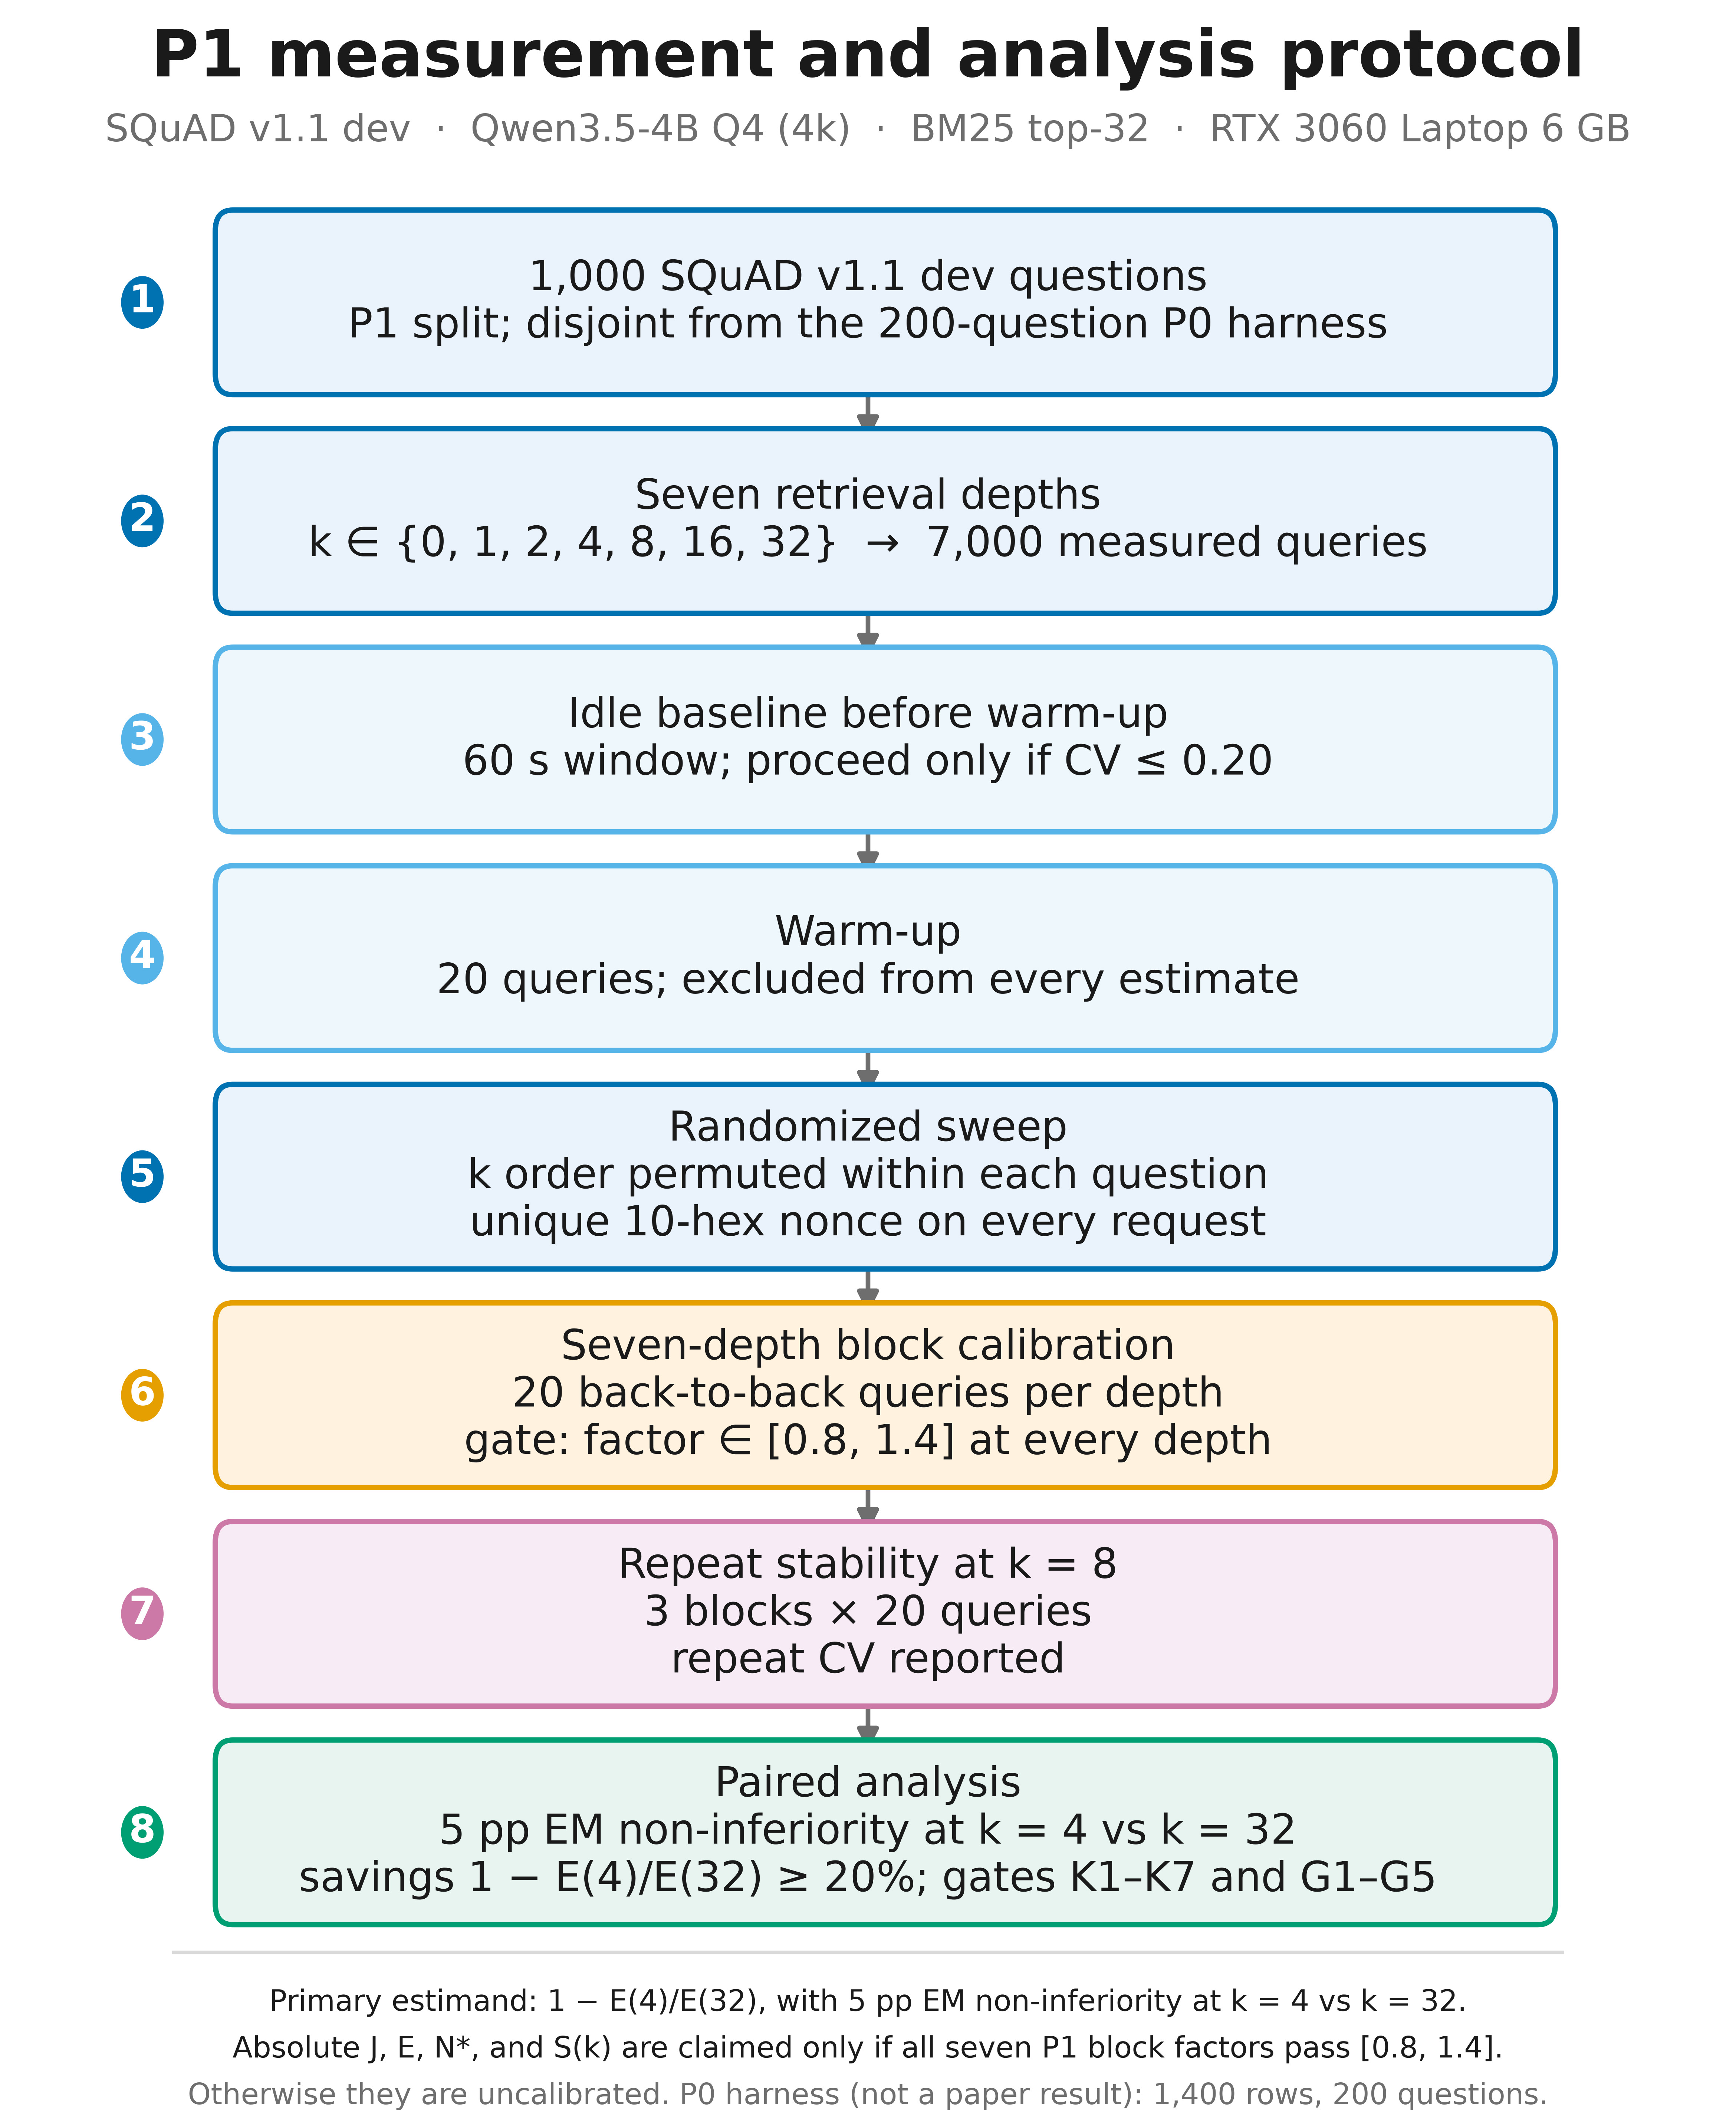
\includegraphics[width=0.82\linewidth]{figures/design.png}}%
    {\missingfigure{figures/design.png}{Design schematic generated by the analysis pipeline; not present in this build.}}
  \caption{Depth sweep and decision. Each question is answered at all seven depths in randomized order with a unique nonce; energy is integrated from NVML with a 0.3~s tail and an idle baseline.}
  \label{fig:design}
\end{figure}

\subsection{Measurement}\label{sec:measurement}

\textbf{Energy decomposition.} For query $q$ at depth $k$ the request energy is decomposed as
\begin{equation}\label{eq:decomp}
  J_{k}(q)=J_{\mathrm{ret},k}(q)+J_{\mathrm{pre},k}(q)+J_{\mathrm{dec},k}(q)+J_{\mathrm{fix}}(q),
\end{equation}
where $J_{\mathrm{ret}}$ is retrieval, $J_{\mathrm{pre}}$ is the prefill of the question and the $k$ passages, $J_{\mathrm{dec}}$ is decoding, and $J_{\mathrm{fix}}$ is the amortized model load and fixed per-query overhead. The GPU sensor captures prefill and decode directly and part of the fixed overhead. BM25 runs on the CPU and is not visible to NVML, so it is estimated by a time-to-joules proxy and reported as an upper bound. The context-side share $S(k)$ uses $J_{\mathrm{ret}}+J_{\mathrm{pre}}$; the retrieval-only share $S_{r}(k)$ uses the proxy alone. They are reported separately and never conflated. \textbf{Sensor and integration.} GPU power is sampled through NVML \cite{nvml} at a 100~ms cadence, together with utilization, memory, temperature, and SM clock. The 100~ms cadence is a sampling label, not 100~ms of independent information: on the pilot laptop the driver updates \texttt{power.draw} at roughly 1~s. Per-query energy is therefore treated as a paired observation, not as a precision measurement. For each query the power samples between the start and the end of the HTTP call are integrated with the trapezoidal rule, the window is extended by a measured post-query tail $\tau=0.3$~s, the idle baseline is subtracted over the same window, and the result is clipped at zero:
\begin{equation}\label{eq:integral}
  J_{\mathrm{gpu}}(q)=\max\!\left(0,\;\int_{t_{0}}^{t_{1}+\tau}P(t)\,dt-P_{\mathrm{idle}}\,(t_{1}+\tau-t_{0})\right).
\end{equation}
where $P(t)$ denotes GPU power at time $t$, $t_{0}$ and $t_{1}$ denote the request start and completion times, $\tau$ denotes the post-query tail, and $P_{\mathrm{idle}}$ denotes the idle baseline. The tail captures the power ramp that a window ending at HTTP completion misses, and it matters most at short depths, where the fixed overhead is a large fraction of the window. Idle is measured before warm-up, not after the run, and the run stops if its coefficient of variation exceeds 0.20.

\textbf{Block calibration.} Per-query windows still miss part of the ramp, and the fraction they miss depends on depth. After the sweep, 20 back-to-back queries are run per depth and integrated as one block. The protocol factor compares the block to the sum of the sweep rows at that depth:
\begin{equation}\label{eq:factor}
  \texttt{factor\_csv}_{k}=\frac{J_{\mathrm{block},k}}{\sum_{i=1}^{20}J_{\mathrm{gpu}}(q_{i},k)},
  \qquad
  \texttt{factor\_block}_{k}=\frac{J_{\mathrm{block},k}}{\sum_{i=1}^{20}W_{\mathrm{block},i}},
  \qquad
  \texttt{consistency}_{k}=\frac{\texttt{factor\_block}_{k}}{\texttt{factor\_csv}_{k}}
\end{equation}
where $J_{\mathrm{block},k}$ denotes the integrated block energy at depth $k$, $W_{\mathrm{block},i}$ denotes the within-block per-query window integral, and the three ratios define the sweep factor, block factor, and consistency diagnostic. The gate is on \texttt{factor\_csv}, in the fixed interval $[0.8,1.4]$. The within-block factor is structurally close to one and can hide a mismatch between the sweep's thermal state and the block's, so it is recorded as a diagnostic and never used as the gate. All seven depths are measured before the gate is evaluated. If every depth passes, the factors are applied and calibrated $J$, $E$, $N^{*}$, and $S(k)$ are primary. If any depth fails, no factor is applied, $J_{\mathrm{gpu,calibrated}}=J_{\mathrm{gpu,raw}}$, and absolute energy is labelled uncalibrated. Mixing calibrated and uncalibrated depths is forbidden, because it would make the ratio depend on which depths happened to pass. \textbf{Prefix cache and thermal state.} Ollama reuses key--value prefixes across requests. In the pilot, a $k=32$ request that followed a $k=16$ request reused the first 16 passages and cut prefill from 710~ms to 247~ms. Every request therefore begins with a unique 10-hex nonce generated from \texttt{secrets.token\_hex(5)}; a missing nonce invalidates the row. The check is directional: prefill at a fixed depth must not fall when the preceding request had a shorter prefix, and a fall is a protocol failure rather than a speedup. Temperature, SM clock, and throttle fraction are logged for every query. The pilot observed the GPU rising from 71.9~$^{\circ}$C to 88.4~$^{\circ}$C, the SM clock falling from 1657~MHz to 1003~MHz, and mean power falling from 82.5~W to 54.2~W, while energy per query remained stable. Depth order is randomized, block calibration is run at the throttled steady state, and the run is cooled between halves. A sensitivity analysis excluding the first 50 queries is reported.

\textbf{CPU proxy and repeatability.} \texttt{pyRAPL} is unavailable on the Windows/AMD host, so BM25 time is measured per query and converted at 20~W single-thread active-above-idle, $J_{\mathrm{ret}}(q)=t_{\mathrm{bm25}}(q)\times 20$~W. The pilot mean was 0.149~s per query, giving 3.11~J per query; at 10--15~W the term would fall to 1.6--2.3~J and lower $E$ by under 1.5\%. The proxy is an upper bound and the retrieval-only share is labelled a proxy share. Repeatability is measured with three repetitions of 20 identical queries at $k=8$, separated by a cooldown applied at the start of every block, and the coefficient of variation is computed per query across repetitions. The pilot median was 3.80\% and the maximum 9.24\%. The minimum detectable effect is approximated as twice the CV, so an effect smaller than that is reported as not measurable and fires K7. \textbf{Wall meter.} A plug-in wall meter would cross-check the integration on a 30-query subset per condition. No meter is available for P0 or P1, and the cross-check is waived under decision D-016. Every energy table in this manuscript therefore states ``wall meter: not measured (waiver)''. The meter is a cross-check in any case: it cannot separate retrieval from generation and is too coarse for per-query attribution.

\subsection{Estimators, Gates, and Inference}\label{sec:estimators}\label{sec:gates}

The descriptive quantities are $A(k)$, $J(k)$, and $E(k)$ from Equation~\eqref{eq:ratio}, with $n_{k}$, $n_{\mathrm{valid}}(k)$, and $n_{\mathrm{invalid}}(k)$ reported at every depth. The primary savings is $\mathrm{Sav}(0.05)=1-\widehat E(4)/\widehat E(32)$, computed as a ratio of sums over the questions with valid rows at both depths. Its interval comes from 10{,}000 paired bootstrap resamples over questions \cite{efron1993bootstrap}, with the question as the resampling unit and the percentile method at 95\%. The same resampling distribution supplies the bootstrap probability that each depth is optimal under the gate, $\Pr(k^{*}=k)$, which is the selection probability that G2 and K3 require.

The accuracy contrast is tested one-sided at $\alpha=0.05$ with the margin as the null value. The null is $A(4)-A(32)\le-0.05$; rejection supports non-inferiority. The paired discordant counts, the paired $n$, and the one-sided lower confidence bound are reported, together with the test statistic. The test is a paired procedure on question-level outcomes, in the family of McNemar's test for correlated proportions \cite{mcnemar1947}, applied to the margin-shifted null. A non-inferiority conclusion requires the lower bound on the difference to exceed $-5$ pp, not merely a point estimate above it. The design and the reporting follow the non-inferiority trial conventions of Piaggio et al.\ \cite{piaggio2006}; the preregistration follows the practice of specifying the analysis before the outcome is observed \cite{nosek2018}.

Only one confirmatory test is declared, so no multiplicity adjustment is applied to it. Secondary estimands (the 2 pp margin, the identity gap, the context share, the affine fit, $N^{*}$, the margin and scoring sensitivities, and the replication) are reported as estimates with intervals and are labelled secondary or exploratory. If a family of confirmatory contrasts were declared, a Holm correction would be required \cite{holm1979}; declaring one test is what makes the single-test error rate the relevant one. The distinction is stated in the tables, not left to the reader.

The calibration rule has two reporting regimes, and the manuscript stays in one of them for the whole run. In the calibrated regime, all seven \texttt{factor\_csv} values lie in $[0.8,1.4]$, the factors are applied, and absolute $J$, $E$, $N^{*}$, and $S(k)$ are claimed. In the uncalibrated regime, at least one factor fails, no factor is applied, and the same quantities are reported as uncalibrated descriptive values that are not claimed. The primary savings and the accuracy contrast are reported in both regimes because they are invariant to a depth-common factor and to calibration respectively. This rule is the reason the P0 failure does not invalidate the confirmatory design, and it is also the reason the failure cannot be hidden: the absolute numbers change regime, while the primary contrast does not.

\begin{algorithm}[H]
  \caption{Preregistered depth sweep, calibration, and primary analysis}
  \label{alg:run}
  \begin{algorithmic}[1]
    \Require frozen config and preregistration hash, question split, depths $\mathcal{K}$, block size $B=20$
    \Ensure registered raw CSV, block factors, primary decision, secondary tables
    \State verify the preregistration and config hashes; refuse to run on a mismatch
    \State measure idle before warm-up; stop if its CV exceeds 0.20
    \For{each question $q$ in the split}
      \State draw a unique 10-hex nonce
      \For{each depth $k\in\mathcal{K}$ in randomized order}
        \State retrieve the top-$k$ passages with BM25 and build the fixed prompt
        \State call the reader; record power from request start to completion plus the 0.3~s tail
        \State integrate, subtract idle, clip at zero, and score normalized exact match
      \EndFor
    \EndFor
    \State run 20 back-to-back queries per depth at the sweep thermal state
    \State compute \texttt{factor\_csv}, \texttt{factor\_block}, and \texttt{consistency} at every depth
    \If{all seven \texttt{factor\_csv} $\in[0.8,1.4]$}
      \State apply the factors; label $J$, $E$, $N^{*}$, and $S(k)$ calibrated
    \Else
      \State apply no factor; label absolute energy uncalibrated; retain the savings ratio
    \EndIf
    \State paired bootstrap over questions (10{,}000 resamples)
    \State one-sided non-inferiority test at $\delta=5$ pp and the 20\% savings floor
    \State \Return the primary decision and the secondary tables
  \end{algorithmic}
\end{algorithm}

The gates were fixed before the confirmatory data were seen and are not re-thresholded after the outcome. A fired gate is a finding and is reported, not tuned away. The kill and reframe gates K1--K7 test whether the depth story is worth telling at all; the go gates G1--G5 test whether the specific policy claim is supported. K1--K4 and K6 firing is a kill or a reframe. K5 and K7 are measurement or framing problems that can be fixed once before they become kills. Table~\ref{tab:gates} lists the criteria and the pilot values.

\begin{table}[pos=htbp]
  \centering
  \caption{Gate definitions fixed before the confirmatory run, with the pilot values. The pilot is prior evidence; the P1 adjudication is in Table~\ref{tab:p1gates}. A fired gate is reported as a finding.}
  \label{tab:gates}
  \footnotesize
  \setlength{\tabcolsep}{4pt}
  \begin{tabular}{@{}l>{\raggedright\arraybackslash}p{6.3cm}>{\raggedright\arraybackslash}p{4.4cm}>{\raggedright\arraybackslash}p{3.4cm}@{}}
    \toprule
    \textbf{Gate} & \textbf{Rule} & \textbf{Pilot value} & \textbf{Reading after pilot} \\
    \midrule
    K1 & Relative energy effect below 10\% & 245\% effect & pass \\
    K2 & $k^{*}$ at the boundary $\{0,K\}$ & $k^{*}=32$ & fail \\
    K3 & $\Pr(k^{*}\ \text{optimal})<0.8$ & 0.61 & fail \\
    K4 & Context share below 5\% and flat & 36.3\% to 85.1\% & pass \\
    K5 & $k^{*}$ spans more than one depth across resamples or datasets & $k^{*}$ spans three gated depths & fail \\
    K6 & Oracle gain below 15\% & 78.8\% (upper bound) & pass \\
    K7 & Repeat CV above 20\%, or MDE above the observed effect & 3.80\% median, 9.24\% max & pass \\
    \midrule
    G1 & 5 pp non-inferiority at an interior $k$, with at least 20\% savings & $k=4$, 69.3\%, no test reported & signal only \\
    G2 & Upper accuracy-loss bound at most 5 pp, and $\Pr(k^{*}\ \text{optimal})\ge0.8$ & selection probability 0.537 & not met \\
    G3 & Context share in $[0.10,0.70]$ at the selected depth, and varying with $k$ & share varies with $k$; value at $k=4$ not recorded & direction only \\
    G4 & Oracle gain at least 20\%, and a learned policy captures at least 50\% & upper bound only; no policy & not evaluated at pilot \\
    G5 & Replication on the 1.5B reader or HotpotQA & not in P1 & not evaluated at pilot \\
    \bottomrule
  \end{tabular}
\end{table}

G1 and G2 are the static-policy gates. They operationalize the preregistered primary hypothesis, H2: at a 5 pp exact-match margin, $k=4$ must not lose more than 5 pp against $k=32$, with at least 20\% energy savings. G1 requires both the accuracy margin and the savings floor, in that order, because the margin is the constraint and the saving is the objective. G2 adds a stability requirement: an upper confidence bound on the accuracy loss within 5 pp, and a bootstrap selection probability of at least 0.8. The pilot failed G2 on the second condition alone, which is why its 5 pp result was a signal rather than a supported claim. P1 adjudicates the same gates in Table~\ref{tab:p1gates}. G3 protects against a degenerate energy split. If the context-side share at the selected depth is below 10\% or above 70\%, the depth lever is either negligible or the measurement is dominated by one component, and the interpretation in Section~\ref{sec:discussion} would not hold. G4 is the adaptive-policy gate; a paper may report G1, G3, and G5 without G4, but it may not claim adaptivity without G4. G5 is the external-validity gate, satisfied by the Qwen2.5-1.5B-Instruct replication or by HotpotQA, not by the exploratory Llama reader and not by the accuracy-only H200 check.

\section{Experiments}\label{sec:experiment}

\subsection{Setup and Dataset}\label{sec:setup}\label{sec:dataset}

All measurements are taken on a single laptop with an NVIDIA RTX 3060 Laptop GPU with 6~GB of memory, running Windows. The GPU is used at batch size one with no concurrent jobs, so a query is never measured while another process shares the device. The reader is the Ollama tag \texttt{qwen3.5:4b} at Q4 quantization with a 4096-token context \cite{ollama}. The retriever is BM25 \cite{robertson2009bm25} over a corpus of 45{,}651 passages built from 70-word chunks of the SQuAD contexts. The prompt template, decoding parameters, chunking, and scoring rule are fixed before the run, and the run manifest records the config hash, the preregistration hash, the model digest, the interpreter, and the idle measurement. The P0 manifest did not record the GPU driver, which is a harness gap: the driver is part of the reporting checklist and must accompany the published manifest before the absolute scale is treated as reproducible. The run seed is 20261115. Depth order is shuffled within each question by that seed. The seed controls only the within-question depth order; the design does not average over seeds, so seed-to-seed variability of the curve is not estimated. Every request carries a unique 10-hex nonce. Power is sampled through NVML at 100~ms, the post-query tail is 0.3~s, idle is measured before warm-up, and the block size is 20 queries per depth. The wall meter is not measured (D-016). Raw run directories are local-only under decision D-020; the repository publishes the registry row, the configs, the manifest, the split IDs, and the aggregate analysis, not the raw CSV or the raw SQuAD text.

The corpus is SQuAD v1.1 \cite{rajpurkar2016squad}. Preparation yields 10{,}570 questions, 20{,}958 contexts, and 45{,}651 passages, the same counts as the pilot. The question splits are disjoint by construction: 200 questions for P0, 1{,}000 for P1, 500 for the reader replication, 200 for the boundary probe, 200 for the context-budget probe, and 150 for the energy-tax arm. P0 is disjoint from P1, and the nested arms are mutually disjoint. The pilot question IDs are not available, so the overlap between the P0 sample and the pilot sample is unknown; by chance it is expected to be about 4 of 200 questions, and the manuscript does not treat the two samples as paired. The P1 sweep is $n=1{,}000$ questions at seven depths, which is 7{,}000 rows; all 7{,}000 were collected with zero invalid rows. The primary analysis population is defined on the question. A valid row requires a non-empty nonce, a completed request, and a power window with no sampler error. A failed or empty generation after a completed request is a wrong answer with $C=0$ and is retained; a row is invalid only for a protocol violation, namely a missing nonce, a request or backend failure, or a sampler error. A model reload inside a run is a backend failure and invalidates the row, because the reloaded model is a different measurement condition. Descriptive $A(k)$, $J(k)$, and $E(k)$ use every sampled question with a valid row at depth $k$, and $n_{\mathrm{valid}}(k)$ and $n_{\mathrm{invalid}}(k)$ are reported at each depth. A question is not dropped from depth $k$ because it lacks a row at another depth. The primary paired test uses questions with valid rows at both $k=4$ and $k=32$, and the paired $n$, the discordant counts, and the invalid counts are reported. There are no outcome-based exclusions: no winsorizing, no trimming, no imputation, and wrong, slow, and throttled answers stay in.

Scoring is normalized exact match for the primary analysis. The pilot used strict exact match, and P0 used the normalized rule; the difference is reported wherever the two are compared, and the accuracy and energy values are never described as like-for-like effects across scoring rules. The secondary scoring sensitivity repeats the primary analysis under lenient span match and under token-level F1 of at least 0.5. The conclusions are required to survive all three rules; a result that exists only under one rule is reported as such.

\subsection{Baselines and Procedure}\label{sec:procedure}

The baseline is the static depth grid of Table~\ref{tab:grid} on the same reader and retriever. The reference depth is $k=32$, the candidate is $k=4$, and the comparison is paired by question. The other depths describe the curve, supply the finite differences for the identity, and enter the affine fit. The 2 pp margin is estimated on the same rows and reported with an interval, without a decision claim. No second reader, no dense retriever, and no learned policy are evaluated in P1. The replication arms were run in P2: Qwen2.5-1.5B-Instruct at $n=500$ and HotpotQA distractor at $n=500$ with $k\le10$ \cite{qwen25,yang2018hotpotqa}. The boundary probe ($k\in\{32,48,64\}$, $n=200$, 8k context) and the 16k context-budget probe are diagnostic; the 16k allocation is a budget, not a 16k-token prompt at $k\le64$. The optional H200 MIG check at 64k is accuracy-only and is never pooled with the RTX 3060 energy results.

The procedure is the one in Algorithm~\ref{alg:run}. The sweep is run first, with no interim look at the accuracy outcome. Block calibration follows the sweep at the same thermal state. The gate is evaluated on all seven factors, and the analysis then runs once, with the preregistration hash checked. The analysis produces the primary decision, the descriptive curve, the identity gap, the context share, the affine fit, $N^{*}$, the margin and scoring sensitivities, and the gate table. The run is registered as \texttt{running} until completion and as \texttt{completed} or \texttt{invalid} afterwards; an aborted run is registered as \texttt{aborted} and is never analysed as if complete.

\subsection{Evaluation Metrics}\label{sec:metrics}

Let $\nu(y)$ be the normalization that lowercases, removes punctuation, removes the articles \emph{a}, \emph{an}, and \emph{the}, and collapses whitespace. The primary correctness rule is normalized exact match,
\begin{equation}\label{eq:em}
  C_{qk}^{\mathrm{EM}}=\mathbf{1}\{\nu(\hat y_{qk})=\nu(y_{q})\}.
\end{equation}
where $\nu(\cdot)$ denotes the normalization, $\hat y_{qk}$ denotes the predicted answer, and $y_{q}$ denotes the gold answer. The secondary rules are lenient span match and token F1,
\begin{equation}\label{eq:lenient}
  C_{qk}^{\mathrm{span}}=\mathbf{1}\{\nu(y_{q})\subseteq\nu(\hat y_{qk})\},
  \qquad
  C_{qk}^{\mathrm{F1}}=\mathbf{1}\{\mathrm{F1}(\hat y_{qk},y_{q})\ge0.5\},
\end{equation}
where, with $\mathcal{T}(y)$ the multiset of normalized tokens,
\begin{equation}\label{eq:f1}
  P=\frac{|\mathcal{T}(\hat y)\cap\mathcal{T}(y)|}{|\mathcal{T}(\hat y)|},
  \quad
  R=\frac{|\mathcal{T}(\hat y)\cap\mathcal{T}(y)|}{|\mathcal{T}(y)|},
  \quad
  \mathrm{F1}=\frac{2PR}{P+R},
\end{equation}
where $\mathcal{T}(\hat y)$ and $\mathcal{T}(y)$ denote the multisets of normalized prediction and gold tokens, $P$ denotes precision, $R$ denotes recall, and $\mathrm{F1}$ denotes their harmonic mean. $\mathrm{F1}=1$ when both token sets are empty and $0$ when either is empty. The primary rule is deliberately conservative: it does not credit a paraphrase, so $A(k)$ is a lower bound on answer quality and $E(k)$ an upper bound. The two secondary rules are sensitivity axes, not alternative primary tests.

Accuracy is a proportion in $[0,1]$ from normalized exact match, and energy is in joules. The per-depth quantities are $A(k)$, $J(k)$, and $E(k)$ from Equation~\eqref{eq:ratio}; $E(k)$ is reported in joules per correct answer. $E(0)$ is reported descriptively but is not used in the fit or the decision, because it divides by the one or two successes at that depth. The savings is the ratio in Equation~\eqref{eq:savings}, reported with a 10{,}000-resample paired percentile interval. The context-side and retrieval-only shares are
\begin{equation}\label{eq:shares}
  S(k)=\frac{J_{\mathrm{ret}}(k)+J_{\mathrm{pre}}(k)}{J(k)},
  \qquad
  S_{r}(k)=\frac{J_{\mathrm{ret}}(k)}{J(k)},
\end{equation}
where $J_{\mathrm{ret}}$ is the CPU BM25 proxy and $J_{\mathrm{pre}}$ is the GPU prefill of the question and the $k$ passages. The proxy is
\begin{equation}\label{eq:proxy}
  J_{\mathrm{ret}}(k)=P_{\mathrm{cpu}}\,t_{\mathrm{ret}}(k),
\end{equation}
with $P_{\mathrm{cpu}}=20$~W and $t_{\mathrm{ret}}$ the measured retrieval wall time. The score is an upper bound, not a measured CPU energy. The identity gap is $\Delta(k)$ from Equation~\eqref{eq:gap}, with a bootstrap interval at the selected depth. The affine fit reports $a$ in joules, $b$ in joules per passage, $R^{2}$, and a lack-of-fit check at the 5\% level, because a high $R^{2}$ on seven means does not by itself establish linearity.

Repeatability is the coefficient of variation of per-query energy across the three repetitions at $k=8$,
\begin{equation}\label{eq:cv}
  \mathrm{CV}=\frac{s}{m},
\end{equation}
where $s$ is the sample standard deviation and $m$ the mean over the three repetitions for a given query; the median and maximum over queries are reported. The implied minimum detectable effect is $2\,\mathrm{CV}$. The block diagnostics are \texttt{factor\_csv}, \texttt{factor\_block}, and \texttt{consistency} from Equation~\eqref{eq:factor}; the gate is on \texttt{factor\_csv} only. Calibration status is reported once per run, not per depth, because the all-or-nothing rule is a property of the run.

\subsection{Statistical Analysis}\label{sec:stats}

The unit of analysis is the question, and every contrast is paired. Let $C_{qk}\in\{0,1\}$ and let $n$ be the number of questions with valid rows at both depths. Define the discordant counts
\begin{equation}\label{eq:discordant}
  b=\sum_{q}\mathbf{1}\{C_{qk}=1,C_{qK}=0\},
  \qquad
  c=\sum_{q}\mathbf{1}\{C_{qk}=0,C_{qK}=1\},
\end{equation}
where $b$ denotes the number of questions correct at depth $k$ and wrong at the reference depth, and $c$ denotes the reverse. The paired mean difference is $\hat d=(b-c)/n$. For paired binary outcomes,
\begin{equation}\label{eq:paired-se}
  \widehat{\mathrm{Var}}(\hat d)=\frac{p_{b}+p_{c}-(p_{b}-p_{c})^{2}}{n},
  \qquad
  \widehat{\mathrm{SE}}(\hat d)=\sqrt{\widehat{\mathrm{Var}}(\hat d)},
\end{equation}
where $p_{b}=b/n$ and $p_{c}=c/n$ denote the discordant proportions. The two-sided interval is $\hat d\pm z_{1-\alpha/2}\widehat{\mathrm{SE}}$, and the one-sided lower bound is $\hat d-z_{1-\alpha}\widehat{\mathrm{SE}}$.

\textbf{Non-inferiority.} For margin $\delta>0$, the null is $H_{0}:d\le-\delta$ and the alternative is $H_{1}:d>-\delta$. The test statistic and one-sided p-value are
\begin{equation}\label{eq:ni-test}
  z_{\mathrm{NI}}=\frac{\hat d+\delta}{\widehat{\mathrm{SE}}(\hat d)},
  \qquad
  p_{\mathrm{NI}}=1-\Phi(z_{\mathrm{NI}}),
\end{equation}
where $\hat d$ denotes the paired mean difference, $\delta$ denotes the non-inferiority margin, $\widehat{\mathrm{SE}}(\hat d)$ denotes its standard error, and $\Phi(\cdot)$ denotes the standard normal cumulative distribution function. Non-inferiority is established at level $\alpha$ when $p_{\mathrm{NI}}\le\alpha$, equivalently when the one-sided lower bound exceeds $-\delta$. A non-significant difference is not non-inferiority: the null is a loss of at least $\delta$, not a loss of zero. \textbf{McNemar and TOST.} The exact McNemar test against $d=0$ uses $b\sim\mathrm{Binomial}(b+c,1/2)$ and is reported as a secondary diagnostic. Equivalence at $\pm\delta$ uses two one-sided tests,
\begin{equation}\label{eq:tost}
  p_{\mathrm{TOST}}=\max\left\{1-\Phi\left(\frac{\hat d+\delta}{\widehat{\mathrm{SE}}}\right),\,
  \Phi\left(\frac{\hat d-\delta}{\widehat{\mathrm{SE}}}\right)\right\},
\end{equation}
where $\Phi(\cdot)$ denotes the standard normal cumulative distribution function and the remaining symbols follow Equation~\eqref{eq:ni-test}. The test is reported only as a sensitivity; the preregistered decision is the one-sided non-inferiority test.

\textbf{Bootstrap.} The primary interval is a paired percentile bootstrap over questions: resample $n$ question indices with replacement, recompute $\hat d$, $E(k)$, the savings, and the selected depth on each resample, and take the $2.5$ and $97.5$ percentiles. A bias-corrected and accelerated (BCa) interval is reported as a sensitivity. The bootstrap is joint: one question-level resample feeds all statistics, so the reported joint probability $\Pr(\text{NI and savings}\ge20\%)$ is not a product of marginal probabilities. \textbf{Selection probability.} On each bootstrap resample, recompute $k^{*}_{\delta}$ from Equation~\eqref{eq:optimum}. The selection probability is
\begin{equation}\label{eq:selection}
  \Pr(k^{*}_{\delta}=k)=\frac{1}{B}\sum_{b=1}^{B}\mathbf{1}\{k^{*(b)}_{\delta}=k\},
\end{equation}
where $B=10{,}000$ denotes the number of bootstrap resamples and $k^{*(b)}_{\delta}$ denotes the selected depth in resample $b$. It is a stability measure, not a posterior probability. A point estimate is reported with $P(k^{*}_{\delta}=k)$ and with the 95\% span of selected depths; an interval that covers two depths is reported as unstable even if the modal depth is clear. \textbf{Power, MDE, and required n.} For a one-sided level-$\alpha$ test with power $1-\beta$, the minimum detectable effect at the observed variance is
\begin{equation}\label{eq:mde}
  \mathrm{MDE}=(z_{1-\alpha}+z_{1-\beta})\,\widehat{\mathrm{SE}},
\end{equation}
where $z_{1-\alpha}$ and $z_{1-\beta}$ denote standard normal quantiles, $\widehat{\mathrm{SE}}$ denotes the standard error of the paired difference, and $\alpha$ and $\beta$ denote the one-sided Type I and Type II error rates. The required number of pairs to detect a true difference $d$ is
\begin{equation}\label{eq:required-n}
  n_{\mathrm{req}}=\frac{(z_{1-\alpha}+z_{1-\beta})^{2}\,\widehat{\mathrm{Var}}(\hat d)}{(d+\delta)^{2}}
\end{equation}
where $\widehat{\mathrm{Var}}(\hat d)$ denotes the estimated variance of the paired difference and $d$ denotes the true difference under the alternative. This is the sample size for the non-inferiority test. At the observed effect, the same formula with $d=\hat d$ gives the sample size needed for the interval to clear the margin; this is the margin frontier of Section~\ref{sec:p1}. The realized power is computed at the observed discordance, not the planning assumption.

\textbf{Multiplicity.} Exactly one confirmatory test is declared, so the family-wise error rate is the single-test error rate. The 2 pp margin, the identity gap, the context share, the affine fit, $N^{*}$, the margin and scoring sensitivities, the replication arms, and the policy analysis are secondary or exploratory. If a family of confirmatory contrasts were declared, a Holm correction would be required; the paper does not declare one. The reporting elements a reader needs to decide whether a depth comparison is reproducible are the preregistration tag, the run and config hashes, the idle and block protocol, the paired counts, the accuracy contrast with its interval, the savings with its calibration status, the selection probability, and the certification cost; Sections~\ref{sec:gates} and~\ref{sec:p1} report each of them.



\section{Results}\label{sec:results}

This section reports the pilot evidence (Section~\ref{sec:pilot}), the P0 harness reproduction (Section~\ref{sec:p0}), the P1 confirmatory result (Section~\ref{sec:p1}), the P2 replication arms, the P3 policy audit, the P4 theory check, and the simulation evidence. The separation is deliberate: the pilot is prior evidence collected before the freeze, P0 is a harness check that produced no claim, and P1 is the confirmatory run. P1 is negative on the primary policy claim and positive on the descriptive energy model; the two are reported separately, and the later arms are labelled descriptive or exploratory so they cannot be mistaken for a second confirmatory test.

\subsection{Pilot, Harness, and Measurement Validity}\label{sec:pilot}

The pilot ran 200 SQuAD v1.1 dev questions at seven depths, 1{,}400 generations, on the local RTX 3060 with the 4-bit Qwen3.5-4B reader and BM25 top-32 over 45{,}651 passages. It is the source of the design, not a confirmatory result: it shows that the energy effect is large and the accuracy effect near the plateau is small, which is why the powered study is sized for accuracy. Table~\ref{tab:pilot} collects the quantities.

\begin{table}[pos=htbp]
  \centering
  \caption{Pilot values (200 SQuAD v1.1 dev questions, seven depths, RTX 3060 Laptop 6~GB, Qwen3.5-4B Q4, BM25 top-32). The readings are the status assigned in the preregistration; none of them is a confirmatory result.}
  \label{tab:pilot}
  \footnotesize
  \setlength{\tabcolsep}{5pt}
  \begin{tabular}{@{}>{\raggedright\arraybackslash}p{4.0cm}>{\raggedright\arraybackslash}p{5.7cm}>{\raggedright\arraybackslash}p{5.0cm}@{}}
    \toprule
    \textbf{Quantity} & \textbf{Pilot value} & \textbf{Reading} \\
    \midrule
    Energy per correct answer & $E(32)=157.1$ vs $E(1)=45.5$ J/correct, $3.45\times$ & steep tradeoff, supported \\
    Affine energy fit & $J(k)=15.74+2.283k$ J, $R^{2}=0.9990$ & supported \\
    Accuracy & $A_{\mathrm{EM}}$ 0.395 ($k=1$) to 0.570 ($k=32$); flat 0.520--0.535 for $k=4$--16 & rises then plateaus \\
    Context-side share & 36.3\% ($k=2$) to 85.1\% ($k=32$) & supported \\
    Optimal-depth identity & gap $+0.044$ at $k=2$, 95\% CI $[-0.050,+0.128]$; $+0.700$ at $k=32$ & holds at 2, fails at 32 \\
    Repeat CV at $k=8$ & median 3.80\%, maximum 9.24\% & supported \\
    Static 2 pp claim & $k^{*}=32$ at the boundary, $\Pr(k^{*}\ \text{optimal})=0.61$ & dead \\
    5 pp selection & $k=4$, 69.3\% savings, $N^{*}=876$, selection probability 0.537 & signal only; did not replicate \\
    Oracle gain & 78.8\% at matched accuracy & upper bound only \\
    \bottomrule
  \end{tabular}
\end{table}

The energy curve is steep and close to affine. Energy per correct answer rises from 45.5 J at $k=1$ to 157.1 J at $k=32$, a factor of 3.45, and the fit $J(k)=15.74+2.283k$ explains $R^{2}=0.9990$ of the variance of the seven depth means. The intercept is 15.74 J per query, so the fixed cost of a request is about seven times the marginal cost of one passage at $k=1$, and the marginal term dominates by $k=8$. The context-side share rises from 36.3\% at $k=2$ to 85.1\% at $k=32$, while the retrieval-only proxy share falls from 17.3\% to 3.5\%. The energy lever is therefore the context that the reader must prefill, not the BM25 scoring, which is the opposite of what a latency-only view of retrieval would suggest.

Accuracy rises from 0.395 at $k=1$ to 0.570 at $k=32$ and is flat between 0.520 and 0.535 for $k=4$ to $16$. Moving from the flat region to the reference depth buys 3.5 to 5.0 pp of exact match, while energy per query more than doubles over the same interval. The shape is what makes the decision interesting: the accuracy gain is real but small, and its size is close to the sampling error at $n=200$. The pilot's minimum detectable effect at that sample size is about 5 pp, so the 2 pp margin was never measurable in the pilot regardless of the point estimate.

The identity behaves as a local diagnostic. At $k=2$ the gap is $+0.044$ with a 95\% interval of $[-0.050,+0.128]$, which includes zero and is consistent with a stationary point near the bottom of the grid. At $k=32$ the gap is $+0.700$, far outside the interval, which says that the marginal energy elasticity at the top of the grid is much larger than the marginal accuracy elasticity. The high-$k$ result is the empirically useful one: it identifies over-retrieval without requiring an accuracy model, and it is consistent with the flat accuracy curve. The low-$k$ result is not a policy recommendation. The identity is computed without the gate, and the 5 pp rule selects $k=4$, not $k=2$.

The two decision rules separate cleanly. At 2 pp the selected depth is 32 at the grid boundary, and the bootstrap probability that 32 is optimal is 0.61, below the 0.8 threshold. The 2 pp rule is dead at this sample size, and the death is a statement about power and selection, not a proof that depth 32 is optimal. At 5 pp the selected depth is 4, with 69.3\% savings and $N^{*}=876$. No non-inferiority test was reported for the pilot, and the selection probability is 0.537, again below 0.8. The 5 pp result is therefore a signal that motivated the powered run. The powered run did not support it: the saving replicated at 58.17\% on the window estimator and 65.25\% on the block estimator, but the accuracy bound fell outside the margin (Section~\ref{sec:p1}).

Two further quantities bound the interpretation. Repeatability at $k=8$ has a median CV of 3.80\% and a maximum of 9.24\%, so the implied minimum detectable effect is about 7.6\% at the median, well below the 245\% energy effect but not negligible for small contrasts. The oracle gain of 78.8\% at matched accuracy is the value of perfect per-question depth selection; it is computed with hindsight and is an upper bound. The pilot trained no learned policy, so the deployable gain from adaptivity is unknown and is not claimed.

\label{sec:p0}

P0 is a harness check, not a result. Its purpose was to reproduce the pilot anchors within 10\% and to verify that the measurement chain, the nonce control, the split, and the registry work end to end. It failed on calibration. The first golden run produced block factors of 0.732 in a cold block and 1.676 in a warm block, and an idle coefficient of variation of 46.4\%. A focused diagnostic measured a stable idle of 14.924~W with 0.9\% CV and a warm block factor of 1.400, which showed that the factor was bimodal rather than borderline: a short block started cold and a block started warm land on opposite sides of the fixed interval. The measurement protocol was then revised under D-019: idle is measured before warm-up, every per-query window carries a 0.3~s tail, the gate is on \texttt{factor\_csv} rather than on the within-block factor, every block is warmed, and a cooldown is applied at the start of every block. A 20-question dry run passed with \texttt{factor\_csv} between 0.834 and 1.380 and consistency between 0.889 and 1.196. An intermediate rerun was aborted after 409 rows because it started from an uncommitted tree and is registered as \texttt{aborted}.

The clean rerun then collected 1{,}400 of 1{,}400 rows with zero invalid rows, 1{,}400 unique nonces, 200 rows at each depth, no model reloads, and a maximum prompt of 3{,}532 tokens against the 4{,}096 context. Its pre-warm-up idle was 15.573~W with a 1.12\% CV, which passes the idle gate. Block calibration then failed at $k=0$ with $\texttt{factor\_csv}=0.7944$, below the fixed 0.8 floor. The raw sum at that depth was 446.672~J, the block was 354.847~J, the within-block factor was 0.9989, and the consistency ratio was 1.2573. No block file, repeatability file, or calibrated analysis was produced, and the run is registered as \texttt{invalid}. Table~\ref{tab:p0checks} lists the checks, and Table~\ref{tab:p0sweep} reports the uncalibrated sweep. Figure~\ref{fig:p0} shows the block factors and the idle baseline.

\begin{table}[pos=htbp]
  \centering
  \caption{P0 harness checks. The first golden run is the pre-revision attempt; the clean rerun is \texttt{\_r3}. ``Not reached'' means the check was not executed because calibration stopped the pipeline.}
  \label{tab:p0checks}
  \footnotesize
  \setlength{\tabcolsep}{4pt}
  \begin{tabular}{@{}>{\raggedright\arraybackslash}p{3.8cm}>{\raggedright\arraybackslash}p{4.0cm}>{\raggedright\arraybackslash}p{4.8cm}>{\raggedright\arraybackslash}p{2.2cm}@{}}
    \toprule
    \textbf{Check} & \textbf{Requirement} & \textbf{Observed} & \textbf{Status} \\
    \midrule
    Passage corpus & exact pilot counts & 10{,}570 / 20{,}958 / 45{,}651 & pass \\
    Manifest & verified, checksums rechecked & status verified & pass \\
    Sweep rows & 1{,}400 & 1{,}400 / 1{,}400 & pass \\
    Invalid rows & 0 & 0 & pass \\
    Nonces & unique 10-hex per request & 1{,}400 unique & pass \\
    Depth coverage & 200 rows at each depth & 200 at each of seven & pass \\
    Model reloads & 0 & 0 & pass \\
    Prompt ceiling & at most 4{,}096 tokens & maximum 3{,}532 & pass \\
    Idle baseline & CV at most 0.20, before warm-up & 15.573~W, CV 1.12\% & pass \\
    Block factor $k=0$ & in $[0.8,1.4]$ & 0.7944 & \textbf{fail} \\
    Block factors $k=1$--$32$ & in $[0.8,1.4]$ & not evaluated & not reached \\
    \texttt{blocks.json} & required & absent & not produced \\
    Repeat CV & three blocks at $k=8$ & not run & not produced \\
    Calibrated $J$, $E$ & required for absolute claims & absent; raw only & not produced \\
    \midrule
    First golden run & factors in $[0.8,1.4]$; idle CV at most 0.20 & 0.732 cold, 1.676 warm; idle CV 46.4\% & \textbf{fail} \\
    \bottomrule
  \end{tabular}
\end{table}

\begin{table}[pos=htbp]
  \centering
  \caption{P0 clean rerun at 200 questions per depth (uncalibrated sweep). No block factor was applied, so $J$ and $E$ are raw and are not claimed.}
  \label{tab:p0sweep}
  \footnotesize
  \setlength{\tabcolsep}{4pt}
  \begin{tabular}{@{}rrrrrr@{}}
    \toprule
    \multicolumn{6}{@{}l}{\emph{Panel A: uncalibrated sweep}} \\
    \midrule
    \textbf{$k$} & \textbf{Valid} & \textbf{Correct} & \textbf{$A(k)$} & \textbf{$J(k)$} & \textbf{$E(k)$} \\
                 &                &                  &                 & \textbf{(J/query)} & \textbf{(J/correct)} \\
    \midrule
    0  & 200 & 0   & 0.000 & 7.77  & --- \\
    1  & 200 & 90  & 0.450 & 15.18 & 33.73 \\
    2  & 200 & 96  & 0.480 & 16.69 & 34.77 \\
    4  & 200 & 101 & 0.505 & 19.80 & 39.21 \\
    8  & 200 & 103 & 0.515 & 27.13 & 52.68 \\
    16 & 200 & 111 & 0.555 & 42.41 & 76.41 \\
    32 & 200 & 105 & 0.525 & 76.15 & 145.05 \\
    \bottomrule
  \end{tabular}
\end{table}

\begin{figure}[pos=htbp]
  \centering
  \IfFileExists{figures/p0_harness.png}%
    {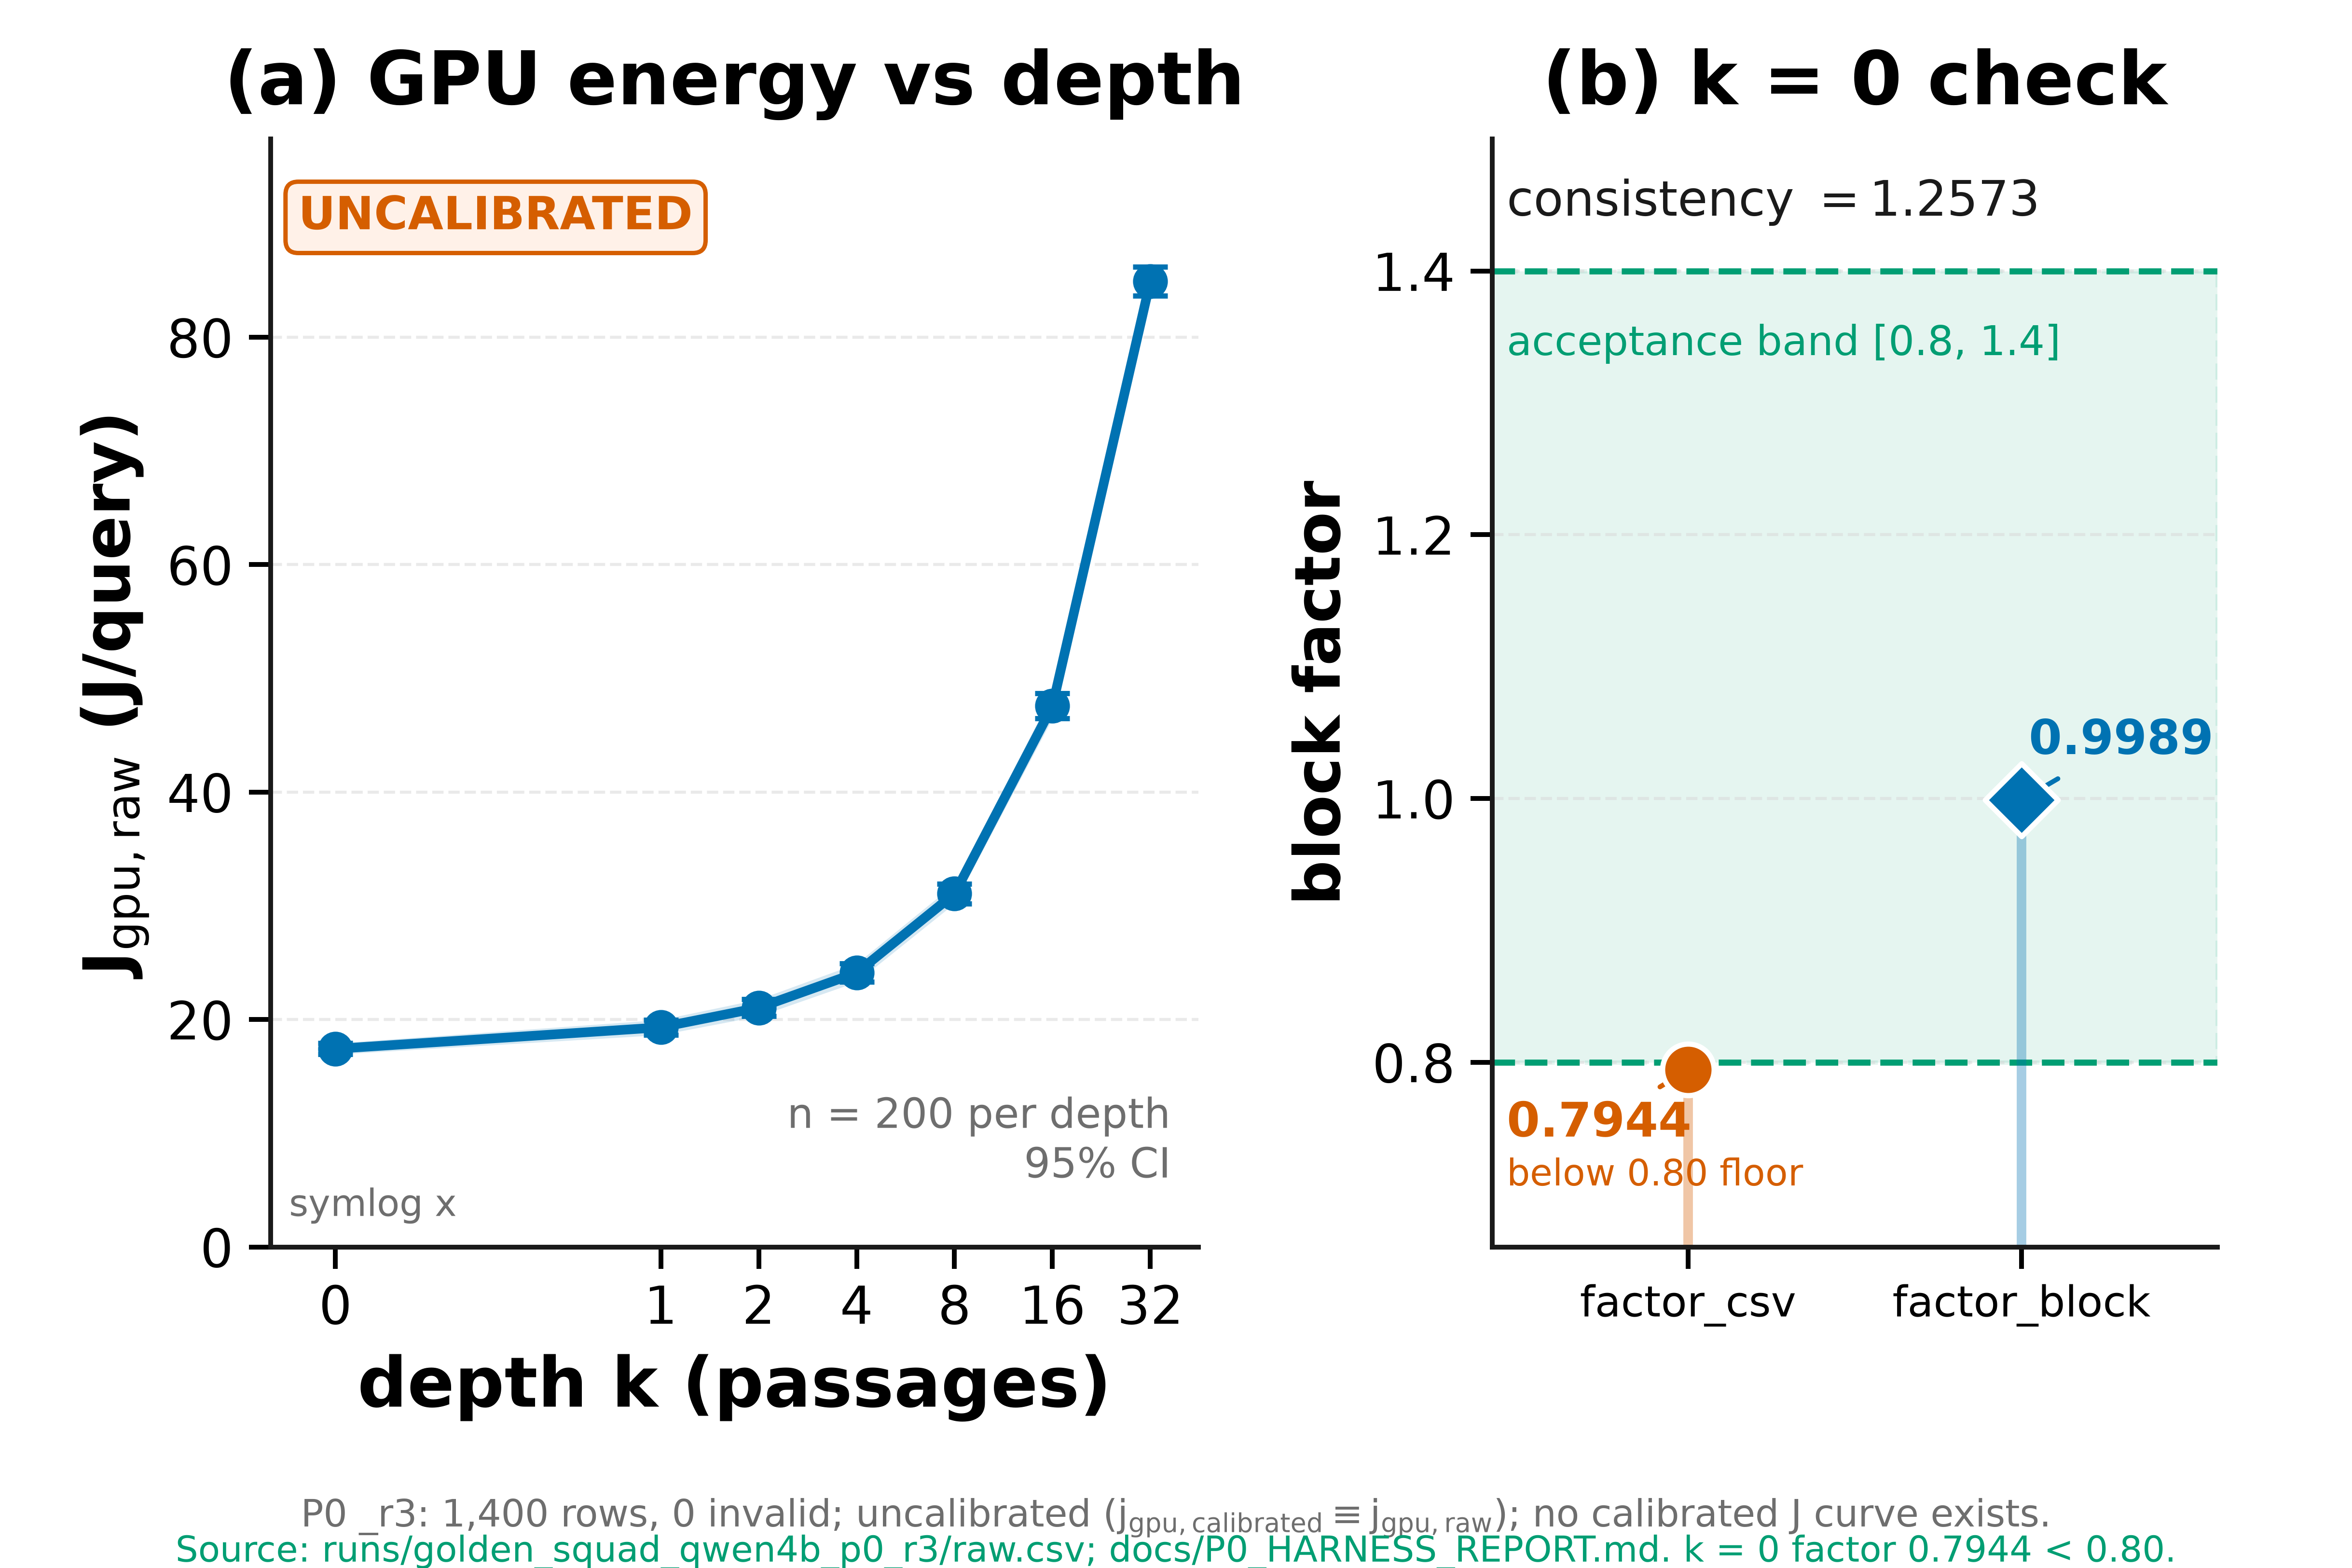
\includegraphics[width=0.98\linewidth]{figures/p0_harness.png}}%
    {\missingfigure{figures/p0_harness.png}{Harness diagnostic figure generated by the analysis pipeline; not present in this build.}}
  \caption{P0 block factors against the fixed $[0.8,1.4]$ gate and the idle baseline. The clean rerun fails at $k=0$ with $\texttt{factor\_csv}=0.7944$.}
  \label{fig:p0}
\end{figure}

The failure is an energy-calibration and thermal-state failure, not a row-collection failure. The sweep is complete, the nonces are unique, the idle baseline is stable, and the prompt fits the context. The discrepancy is between the two window types: the sweep's per-query windows sum to 446.672~J at $k=0$, while the 20-query block integrates to 354.847~J, so the per-query sum exceeds the block by 25.9\%. The within-block factor of 0.9989 shows that the block integration itself is internally consistent, which is why the within-block factor is a diagnostic and not the gate. At short depths the per-query window is dominated by fixed overhead, and a 100~ms sampler with a one-second driver update cannot resolve the ramp; a block that runs back-to-back measures a different window. The first run's bimodal factors point to the same thermal/window-state mismatch.

The anchor comparison in Table~\ref{tab:p0sweep} is reported for completeness and is not adjudicable. The raw $J$ values are 15.0--21.1\% below the calibrated pilot anchors, the affine intercept is 29.5\% low, and the slope is 11.4\% low, all outside the 10\% tolerance. Because no factor was applied, these differences confound the reader, the thermal state, the scoring rule, and the calibration. The $R^{2}$ of the raw fit is 0.9941 and passes its check, which says that the shape of the curve is reproduced even when its scale is not. The accurate statement is that the harness measures rows reliably but does not reproduce the pilot's absolute energy calibration. The 0.7944 value is 0.0056 below the floor; the gate is not re-thresholded because the outcome is known, and the run remains \texttt{invalid}.

The consequence for the rest of the manuscript is a reporting rule, not a repair. Absolute $J$, $E$, $N^{*}$, and $S(k)$ are withheld unless all seven P1 block factors pass. The primary savings $1-E(4)/E(32)$ is reported in either case, because a depth-common factor cancels in the ratio. P1 ran on 2026-11-15 on the principal investigator's authority as a documented reversal (D-022), not because P0 passed, and it passed all seven block factors; its calibrated result is in Section~\ref{sec:p1}. The preregistration records the P0 failure and the calibration-invariant contrast in its pre-freeze revision log.

\label{sec:validity}

The P2 calibration failures motivated a direct probe of the per-query window. With a continuous sampler and a 3~s quiet window after each query, the power signal did not return to the pre-run idle: the residual was 5.0~W at $k=0$, 10.3~W at $k=8$, and 14.6~W at $k=32$ after 2--3~s, and the pre-query floor was 5--64~W above idle depending on the preceding depth. A second probe on the P1 Ollama reader shows the same pattern (pre-query 4.5--55.6~W; residual 6.9--16.0~W after 3~s). A query's measured energy must not depend on which query preceded it. In the P1 and P2 sweeps, the $k=0$ energy varies with the previous row's depth by 24\% (P1), 48\% (Qwen1.5B), 22\% (HotpotQA), and 82\% (Llama). Figure~\ref{fig:validity} shows both diagnostics.

\begin{figure}[pos=htbp]
  \centering
  \IfFileExists{figures/measurement_validity.png}%
    {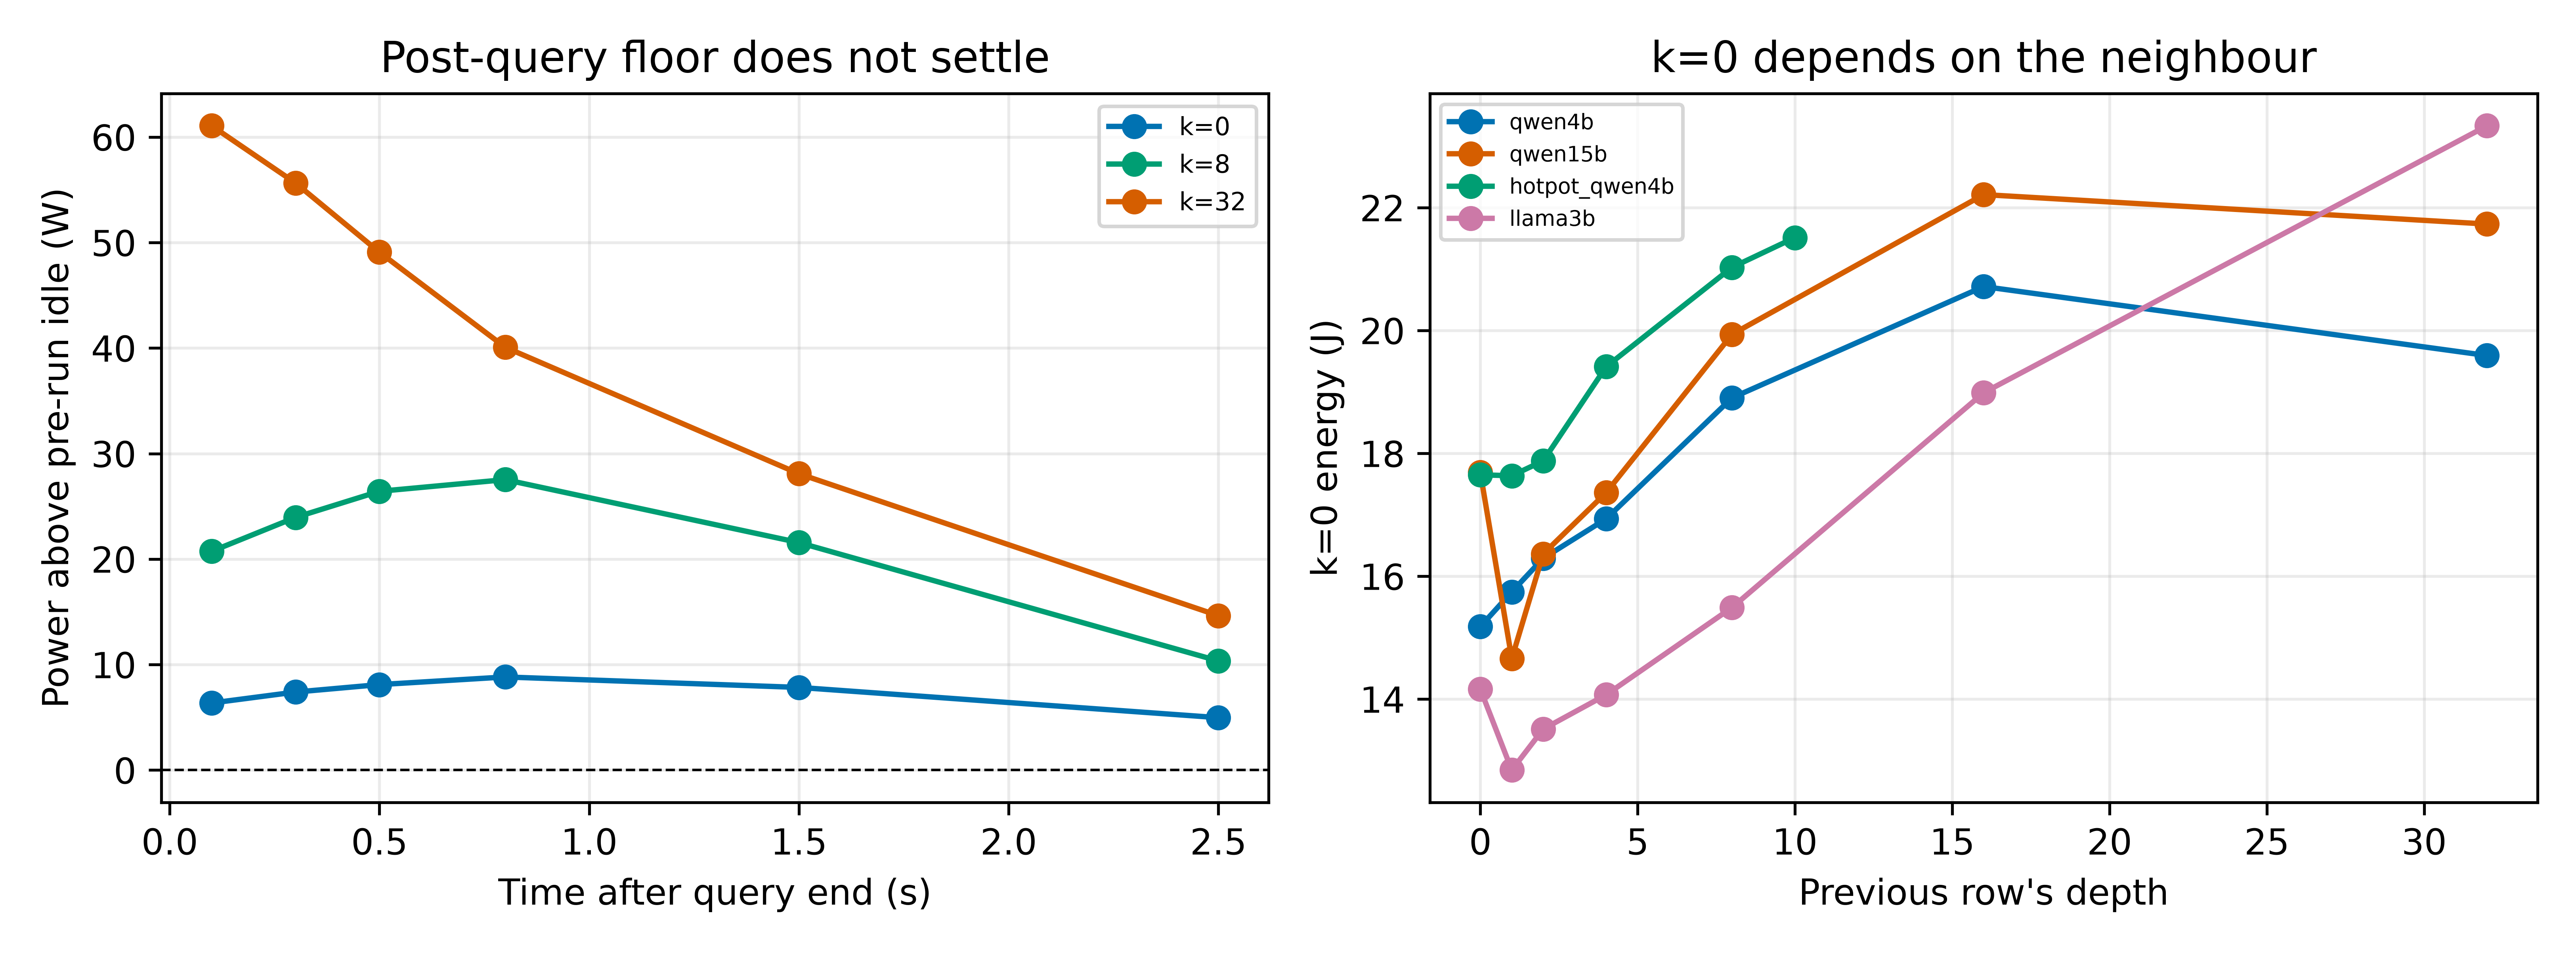
\includegraphics[width=0.98\linewidth]{figures/measurement_validity.png}}%
    {\missingfigure{figures/measurement_validity.png}{Measurement-validity figure generated from the probe.}}
  \caption{Left: the post-query power floor does not return to the pre-run idle within 3~s. Right: $k=0$ energy depends on the preceding row's depth. Both are diagnostics of the per-query estimator, not of the reader.}
  \label{fig:validity}
\end{figure}

The replay does not survive replication. A single replay of the sweep's depth permutation as one continuous block gave 7{,}336.9~J, within 2.0\% of the 7{,}195.7~J block sum, and an earlier draft read that as decisive. Ten independent replays show it is a coincidence: the replay-to-block ratio has median 0.847 (range 0.786--1.036) and drifts with thermal position (Spearman $\rho=-0.855$), from 1.036 on the coolest GPU to 0.79--0.82 on the last three. The depth-resolved replay energies are per-query window sums recovering 0.469 of block energy at $k=1$ and 0.820 at $k=32$, the same depth-dependent bias as the sweep but larger. Table~\ref{tab:bounded} reports savings from both estimators. The qualitative saving is robust: every arm is above the 20\% floor under both. The point value is not, and 3~pp agreement is unattainable when the references are themselves non-stationary. We retain the block estimator on stability grounds, report P2 energy as a range, and treat P1's absolute $J$ as provisional because its $k=0$ factor is 1.1\% above the floor. The accuracy contrast and the qualitative saving are unaffected.

\begin{table}[pos=htbp]
  \centering
  \caption{Bounded savings from the sweep and block estimators. Accuracy is the same in both columns; only the energy estimator changes.}
  \label{tab:bounded}
  \footnotesize
  \begin{tabular}{@{}llrr@{}}
    \toprule
    \textbf{Arm} & \textbf{Contrast} & \textbf{Sweep} & \textbf{Block} \\
    \midrule
    P1 Qwen4B & 4 vs 32 & 68.5\% & 64.3\% \\
    Qwen1.5B & 4 vs 32 & 92.1\% & 90.9\% \\
    HotpotQA & 4 vs 10 & 23.0\% & 31.4\% \\
    Llama 3B & 4 vs 32 & 68.9\% & 77.3\% \\
    \bottomrule
  \end{tabular}
\end{table}

\begin{table}[pos=htbp]
  \centering
  \caption{Block estimator on 1{,}000 disjoint questions per depth. Every joule is GPU energy from NVML; absolute values remain a range.}
  \label{tab:p7blocks}
  \footnotesize
  \begin{tabular}{@{}rrrrr@{}}
    \toprule
    $k$ & $A(k)$ & GPU energy/query (J) & $E(k)$ (J/correct) & CV \\
    \midrule
    0  & 0.002 & 8.59  & --     & 3.6\% \\
    1  & 0.386 & 20.40 & 52.84  & 7.0\% \\
    2  & 0.420 & 22.65 & 53.92  & 5.2\% \\
    4  & 0.459 & 28.33 & 61.72  & 4.3\% \\
    8  & 0.465 & 37.44 & 80.52  & 4.0\% \\
    16 & 0.479 & 54.50 & 113.78 & 4.3\% \\
    32 & 0.490 & 87.04 & 177.64 & 1.2\% \\
    \bottomrule
  \end{tabular}
\end{table}

The block design provides the estimate we do report (Table~\ref{tab:p7blocks}). With five randomized blocks of 200 disjoint questions at each of the seven depths (1{,}000 questions per depth, 7{,}000 measured requests, 120~s cooldown between blocks), the saving is 65.25\% of GPU energy per correct answer at $k=4$ against $k=32$, with a cluster-bootstrap 95\% interval of [61.27, 69.11] over 35 blocks. Block-to-block CV is 1.2--7.0\% at every depth and the affine slope is $2.131$ J per passage, $[2.043, 2.219]$. Its accuracy is monotone and reproduces the confirmatory sample within 0.9~pp at every depth, so the disagreement with the sweep is an estimator effect, not a sampling effect. Two properties support it where the agreement test could not, both in Section~\ref{sec:limitations}: session variance is negligible under cooldown separation, and the saving is reproducible to about one percentage point across occasions while the joule level moves 3--6\%.

The depth curve is a knee rather than an interior optimum. $E(k)$ is minimised at $k=1$ (52.84) with $k=2$ effectively tied (53.92), because accuracy still rises steeply there: $k=1$ to $k=2$ adds 3.4~pp for 2.0\% more energy, $k=2$ to $k=4$ adds 3.9~pp for 14.5\% more, and $k=8$ to $k=32$ adds 2.5~pp for 120.6\% more. This is a property of this dataset, reader, and retriever, not a universal $k^{*}$.

\subsection{Confirmatory, Descriptive, and Replication Results}\label{sec:p1}

The P1 sweep ran 1{,}000 SQuAD v1.1 dev questions at seven depths on 2026-11-15 under the frozen preregistration (\texttt{prereg-freeze-v1}, hash \texttt{fb9e5bcf\ldots}) and the reversal recorded in D-022. It collected 7{,}000 of 7{,}000 rows with zero invalid rows and all 1{,}000 questions at all seven depths. All seven block factors passed the fixed $[0.8,1.4]$ gate and were applied: 0.8089, 1.2506, 1.2403, 1.3111, 1.2902, 1.2143, and 1.0587 for $k=0$ to $32$. The $k=0$ factor is only 1.1\% above the 0.8 floor, and it is reported as measured. Idle was 15.794~W with a 1.23\% CV, and the repeatability check at $k=8$ gave a median CV of 2.81\%, a maximum of 18.44\%, and an implied minimum detectable effect of 5.62\%, below the 20\% threshold. The calibrated regime therefore applies to the whole run, and absolute $J$, $E$, $N^{*}$, and $S(k)$ are reported as calibrated. Table~\ref{tab:p1outputs} gives the primary decision.

\begin{table}[pos=htbp]
  \centering
  \caption{P1 primary decision at $n=1{,}000$: 5 pp accuracy margin, 20\% savings floor, one-sided lower bound, and bootstrap savings interval.}
  \label{tab:p1outputs}
  \footnotesize
  \setlength{\tabcolsep}{4pt}
  \begin{tabular}{@{}>{\raggedright\arraybackslash}p{3.9cm}>{\raggedright\arraybackslash}p{3.2cm}>{\raggedright\arraybackslash}p{5.2cm}>{\raggedright\arraybackslash}p{2.9cm}@{}}
    \toprule
    \textbf{Quantity} & \textbf{Estimate} & \textbf{95\% interval or test} & \textbf{Outcome} \\
    \midrule
    $A(4)$ & 0.450 & paired $n=1{,}000$ & --- \\
    $A(32)$ & 0.493 & --- & --- \\
    $A(4)-A(32)$ & $-4.30$ pp & one-sided lower bound $-6.17$ pp; $p=0.2691$ & gate not met ($-5$ pp) \\
    Savings $1-E(4)/E(32)$ & 58.17\% & [56.02, 60.14]\% & floor met (20\%) \\
    Savings, block estimator & 65.25\% & [61.27, 69.11]\% & floor met (20\%) \\
    \midrule
    Policy decision & --- & both conditions required & \textbf{not supported} \\
    \midrule
    2 pp estimate & $-4.30$ pp & lower bound $-6.17$ pp; $p=0.9785$ & not supported \\
    $N^{*}$ & 6{,}189 queries & [5{,}697, 6{,}748] & $C_{\mathrm{cert}}=311{,}992$ J \\
    \bottomrule
  \end{tabular}
\end{table}

The accuracy contrast is the decisive quantity. The paired population is all 1{,}000 questions; 44 pairs favour $k=4$ and 87 favour $k=32$, for a mean difference of $-4.30$ pp. The point estimate is inside the 5 pp margin by 0.70 pp, but the one-sided 95\% lower bound is $-6.17$ pp, which is 1.17 pp outside the margin, and the one-sided test of the null that the loss is at least 5 pp gives $p=0.2691$. The null is therefore not rejected. The correct statement is that non-inferiority is not established at 5 pp; it is not a demonstration that the true loss exceeds 5 pp. The same paired contrast is clearly nonzero in the other direction: its two-sided 95\% interval is [$-6.53$, $-2.07$] pp and the exact McNemar test gives $p=0.0002$. The data therefore establish a measurable accuracy cost, while leaving the 5 pp bound unresolved. The observed discordance is 13.1\% (131 of 1{,}000 pairs), above the 8\% used in the planning calculation, which widens the interval and explains why a design powered at 8\% discordance did not resolve the margin. Because SQuAD questions share contexts, the interval was recomputed with a context-clustered standard error: 806 clusters, design effect 0.98, cluster SE 1.13~pp, 95\% CI $[-6.51,-2.09]$~pp. Clustering leaves the conclusion unchanged. The 2 pp contrast has the same point estimate and lower bound and $p=0.9785$; it is estimation-only and is also not supported. H2 is therefore not supported: the savings condition is met and the accuracy condition is not. Figure~\ref{fig:contrasts}(a) puts the three accuracy contrasts on one scale.

The exploratory inference layer agrees. A restricted-MLE score test gives $p=0.2703$ and an exact unconditional sensitivity gives $p=0.4182$; TOST fails at $\pm5$ pp ($p=0.2691$) and at $\pm2$ pp ($p=0.9785$); the BCa interval for the mean difference is $[-6.60,-2.20]$ pp and for the savings $[55.99,60.10]$%. The joint question bootstrap puts the probability of (5 pp NI and $\ge20$\% savings) at 0.154. At the observed discordance, realized power at $d=-4.3$ pp is 0.152, and 80\% power would require about 16{,}300 pairs (50\% power about 7{,}130). These are sensitivity quantities; the confirmatory verdict is unchanged. Energy, in contrast, clears its floor with room to spare. The calibrated saving is 58.17\% with a 95\% interval of [56.02, 60.14]\%, well above the 20\% floor. The policy decision requires both conditions, and since the accuracy gate fails, the decision is \textbf{not supported}. The saving is real as a descriptive quantity; it is not attached to an accuracy guarantee that this sample can support.

\textbf{Descriptive curve.} Table~\ref{tab:p1desc} reports the calibrated curve. Energy per correct answer rises from 73.71 J at $k=1$ to 192.59 J at $k=32$, a factor of 2.61, and energy per query rises from 28.82 to 94.95 J over the same interval. Fitting the six positive depths gives $J(k)=26.90+2.149k$, with 95\% intervals $[25.85,27.95]$ for the intercept and $[2.055,2.243]$ for the slope and a weighted $R^{2}=0.999$; including the $k=0$ floor gives $J=24.0759+2.2772k$ with $R^{2}=0.9714$ and a lack-of-fit $F=1.549$, $p=0.2813$. Linearity is not rejected and H1 is supported. The intercept is higher and the fit is noisier than in the pilot ($a=15.74$, $R^{2}=0.9990$); the difference is descriptive, because the pilot and P1 differ in sample size, calibration factors, and thermal state. The context-side share rises from 0.209 at $k=1$ to 0.807 at $k=32$, is 0.355 at the selected depth, and is not flat; H4 is supported. The $k=0$ row rests on a single correct answer ($A=0.001$), so its $E$ value is not interpretable as a cost and is excluded from the fit and the decision. Figure~\ref{fig:p1} plots the three curves.

\textbf{Depth or tokens?} Prompt length, not passage count as such, carries the energy. Mean prompt tokens rise from 86 at $k=0$ to 2{,}769 at $k=32$ and correlate with depth at 0.993. A model in prompt tokens, $J=21.83+0.0272T$, fits better than the depth model ($R^{2}=0.902$ versus 0.888; BIC 29{,}290 versus 30{,}212). In a model with both regressors the depth coefficient is $-0.11$~J/passage (cluster SE 0.11), indistinguishable from zero, while the token coefficient stays at 0.0285. Depth is the control knob, but the physical cost is context length, so the same energy model should transfer to another retriever or reader through token count. This also explains why the intercept rather than the slope moved between pilot and P1.

\begin{table}[pos=htbp]
  \centering
  \caption{P1 descriptive results per depth, calibrated. $J$ is GPU energy plus the CPU proxy; $E$ is the ratio of sums; $S$ is the context-side share.}
  \label{tab:p1desc}
  \footnotesize
  \setlength{\tabcolsep}{5pt}
  \begin{tabular}{@{}rrrrr@{}}
    \toprule
    \textbf{$k$} & \textbf{$A(k)$} & \textbf{$J(k)$ (J/query)} & \textbf{$E(k)$ (J/correct)} & \textbf{$S(k)$} \\
    \midrule
    0  & 0.001 & 14.59 & 14{,}585.49 & 0.000 \\
    1  & 0.391 & 28.82 & 73.71  & 0.209 \\
    2  & 0.417 & 30.58 & 73.33  & 0.271 \\
    4  & 0.450 & 36.25 & 80.56  & 0.355 \\
    8  & 0.467 & 44.63 & 95.58  & 0.492 \\
    16 & 0.481 & 62.17 & 129.26 & 0.646 \\
    32 & 0.493 & 94.95 & 192.59 & 0.807 \\
    \bottomrule
  \end{tabular}
\end{table}

\begin{figure}[pos=htbp]
  \centering
  \IfFileExists{figures/p1_curve.png}%
    {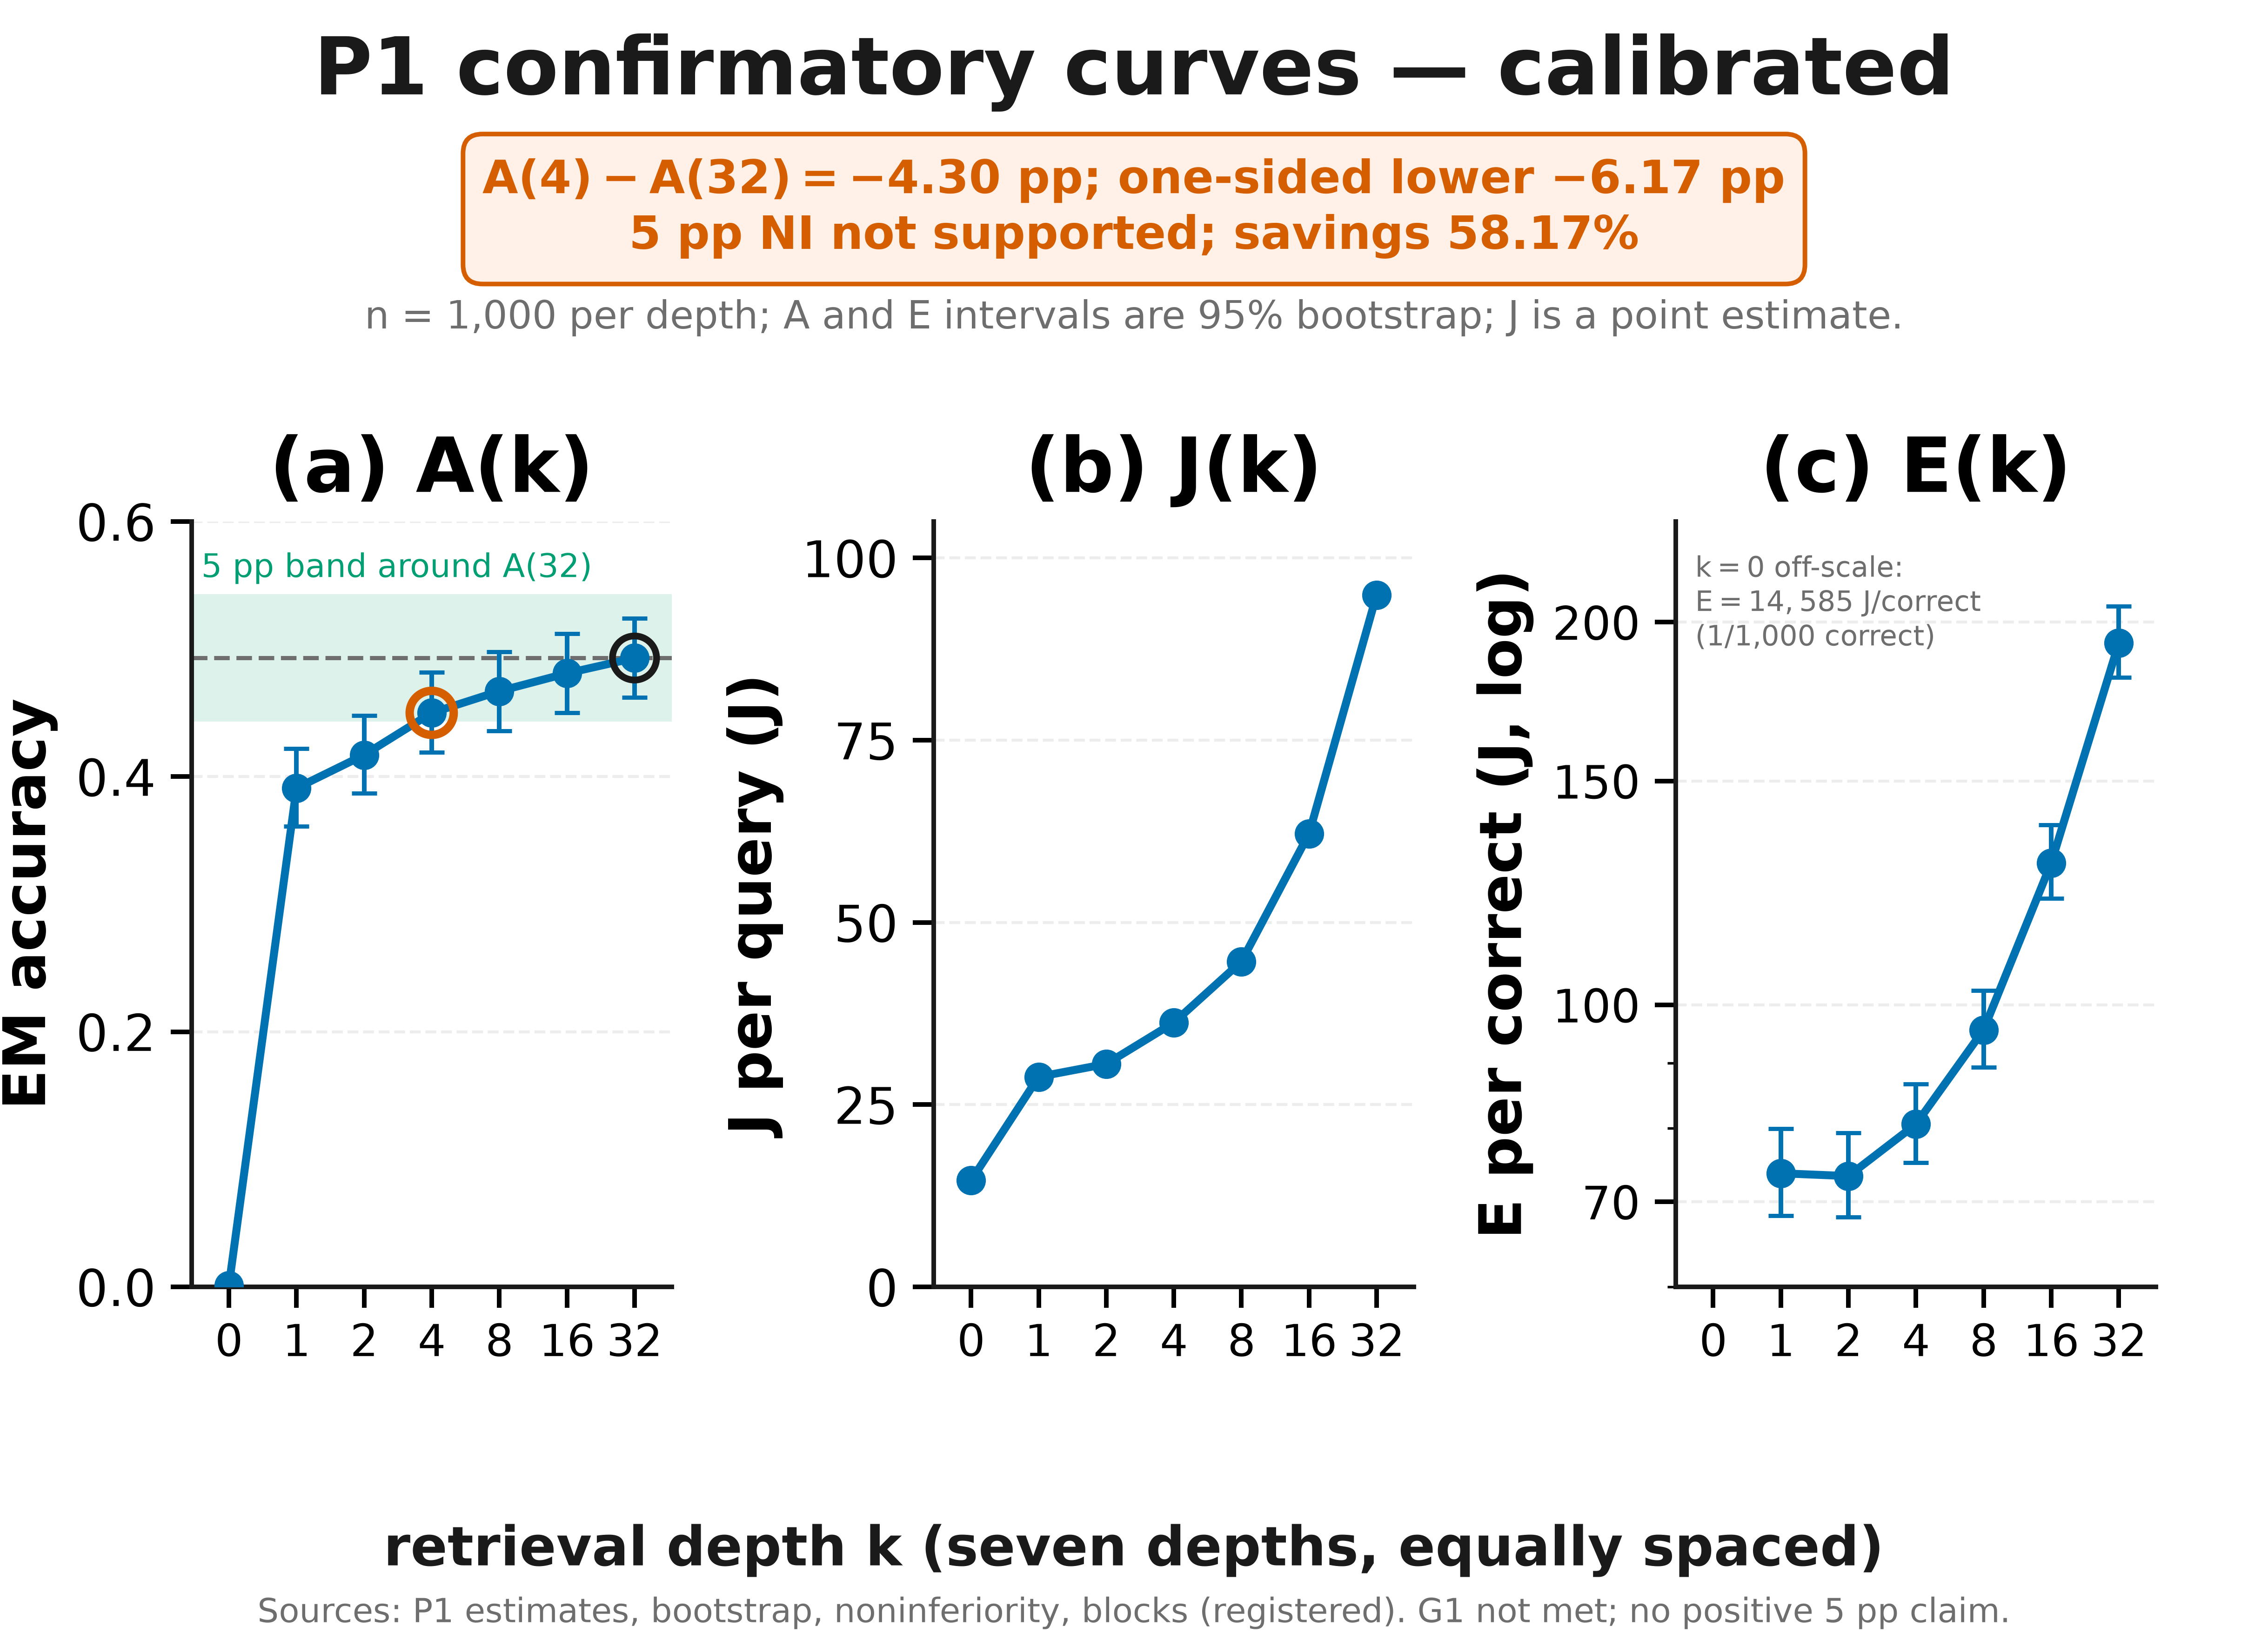
\includegraphics[width=0.98\linewidth]{figures/p1_curve.png}}%
    {\missingfigure{figures/p1_curve.png}{P1 curve generated from the registered analysis.}}
  \caption{P1 curves: accuracy $A(k)$, energy per query $J(k)$, and energy per correct answer $E(k)$ at the seven depths, calibrated.}
  \label{fig:p1}
\end{figure}

\textbf{Identity and selection.} The identity gap at $k=4$ is $+0.2004$ with a 95\% interval of $[0.1677,0.2320]$, which excludes zero; H3 is not supported. A positive gap means that the energy elasticity exceeds the accuracy elasticity at the selected depth, so the unconstrained ratio is already rising where the gate selects. This is a diagnostic failure, not a contradiction of the policy result. The gate, not the identity, chooses the depth, and the identity says that the chosen depth is above the unconstrained energy optimum. The selection is also unstable. The bootstrap probability of optimality is 0.0237 at $k=2$, 0.7244 at $k=4$, 0.2433 at $k=8$, and 0.0086 at $k=16$; all other depths have probability zero. The 5 pp selection therefore reaches 72.4\% at $k=4$, below the 0.8 threshold, and $k=8$ takes 24.3\%. The instability has a concrete source: $k=4$ clears the accuracy gate by only 0.70 pp, so a small resampling movement in $A(4)$ pushes the smallest feasible depth to $k=8$, whose $E$ is higher. K3 fails on the 0.8 threshold, and K5 fails because the 95\% span covers both $k=4$ and $k=8$. The point estimate of the selected depth is stable in the sense that $k=4$ is the modal choice, but it is not stable enough for the preregistered criterion. Two selection notions are worth separating. The preregistered bootstrap probability resamples the curve and asks how often each depth is optimal; it is 0.7244 and K3 fails. A cross-fitted deployment rule, which selects the smallest depth clearing 5~pp and 20\% on four folds and is scored on the fifth, is stable: all five folds select $k=4$, the held-out saving is 58.13\% (SD 1.96), and the winner's curse is 0.03~pp. The gate failure is about the stability of the argmin under resampling, not about whether a practitioner would land on $k=4$.

\textbf{Gate adjudication.} Table~\ref{tab:p1gates} reports the gates. The measurement gates and the descriptive gates pass: K1 (1.613, a 161\% relative energy effect between $k=1$ and $k=32$), K2 ($k=4$, interior), K4 ($S(4)=0.355$, not flat), K7 (maximum repeat CV 18.44\%, MDE 5.62\%), and G3 ($S(4)=0.355$ in $[0.10,0.70]$ and rising). The policy gates fail: K3 (0.7244), K5 (span 4, $k=4$ and $k=8$), G1 (accuracy gate not met although savings are 58.17\%), and G2 (upper bound on loss 6.17 pp and $P=0.7244$). K6 passes on the unconstrained P3 oracle gain (36.80\%, above the 15\% floor); G4 uses the matched-accuracy 28.64\% gap and fails because the policy saving is negative ($-0.71$\%), a capture of $-9.8$\% (95\% CI $-22.8$ to $-1.8$) against the matching no-abstention gap (the earlier $-2.46$\% divided the same saving by the abstention-inclusive gap), and G5 is evaluated in Section~\ref{sec:p2} and passes via HotpotQA. The pattern is consistent: the measurement and descriptive claims are supported, the static policy claim is not, and the direction replicates on the multi-hop arm but not on the 1.5B reader.

\begin{table}[pos=htbp]
  \centering
  \caption{P1 gate adjudication. Criteria were fixed before the run and are not re-thresholded. K6 and G4 use the P3 oracle and policy analysis; G5 is evaluated in Section~\ref{sec:p2} and passes via HotpotQA.}
  \label{tab:p1gates}
  \footnotesize
  \setlength{\tabcolsep}{4pt}
  \begin{tabular}{@{}l>{\raggedright\arraybackslash}p{5.9cm}>{\raggedright\arraybackslash}p{6.0cm}>{\raggedright\arraybackslash}p{2.2cm}@{}}
    \toprule
    \textbf{Gate} & \textbf{Fail if} & \textbf{P1 observation} & \textbf{Outcome} \\
    \midrule
    K1 & relative energy effect $<10$\% & 1.613 (161\%) & pass \\
    K2 & $k^{*}$ at boundary $\{0,K\}$ & $k=4$, interior & pass \\
    K3 & $\Pr(k^{*}\ \text{optimal})<0.8$ & 0.7244 & fail \\
    K4 & context share $<5$\% and flat & 0.355, rising & pass \\
    K5 & $k^{*}$ spans more than one depth & 95\% span 4 ($k=4$, $k=8$) & fail \\
    K6 & oracle gain $<15$\% & 36.80\% & pass \\
    K7 & repeat CV $>20$\% or MDE $>$ effect & maximum 18.44\%, MDE 5.62\% & pass \\
    \midrule
    G1 & 5 pp test fails or savings $<20$\% & gate not met; savings 58.17\% (window), 65.25\% (block) & fail \\
    G2 & loss bound $>5$ pp or $\Pr<0.8$ & 6.17 pp; 0.7244 & fail \\
    G3 & context share outside $[0.10,0.70]$ or flat & 0.355, rising & pass \\
    G4 & oracle $<20$\% or policy capture $<50$\% & 28.64\% matched; $-9.8$\% & fail \\
    G5 & neither replication arm replicates & HotpotQA, $-10.80$ pp & pass \\
    \bottomrule
  \end{tabular}
\end{table}

\textbf{Certification and sensitivity.} The certification cost at $k=4$ is $N^{*}=6{,}189$ queries with a 95\% interval of $[5{,}697,6{,}748]$, using $C_{\mathrm{cert}}=311{,}992$~J for the sweep. This is the break-even volume: the measured sweep energy is repaid after about 6{,}200 deployment queries if the point-estimate saving held. The calculation is descriptive because the accuracy gate failed; it is not a deployment guarantee. Table~\ref{tab:p1sens} reports the margin and scoring sensitivity. The selected depth is rule-dependent: exact match at 2 pp selects $k=16$ (32.9\%), 3--4 pp select $k=8$ (50.4\%), 5--6 pp select $k=4$ (58.2\%), and 8--10 pp select $k=2$ (61.9\%). At the primary 5 pp margin, lenient span match selects $k=8$ (49.9\%) and token F1 of at least 0.5 selects $k=8$ (50.6\%). No rule selects $k=32$, so the qualitative statement that the maximum depth is never the selected depth survives all three scoring rules; the selected depth itself does not. The frontier prices the guarantee directly: tightening the margin from 8 to 6~pp costs 3.75~pp of saving, from 4 to 3~pp costs 7.80~pp, and from 3 to 2~pp costs 17.49~pp. The marginal price of accuracy rises sharply below 5~pp, which makes 5~pp the cheapest defensible guarantee on this curve rather than an arbitrary choice.

\begin{table}[pos=htbp]
  \centering
  \caption{Sensitivity of the selected static depth to the accuracy margin and scoring rule at $n=1{,}000$. The primary rule is exact match at 5 pp. No rule selects $k=32$.}
  \label{tab:p1sens}
  \footnotesize
  \setlength{\tabcolsep}{6pt}
  \begin{tabular}{@{}llrr@{}}
    \toprule
    \textbf{Rule} & \textbf{Margin} & \textbf{Selected $k$} & \textbf{Savings} \\
    \midrule
    Exact match & 2 pp & 16 & 32.9\% \\
    Exact match & 3 pp & 8 & 50.4\% \\
    Exact match & 4 pp & 8 & 50.4\% \\
    Exact match & 5 pp & 4 & 58.2\% \\
    Exact match & 6 pp & 4 & 58.2\% \\
    Exact match & 8 pp & 2 & 61.9\% \\
    Exact match & 10 pp & 2 & 61.9\% \\
    \midrule
    Lenient span & 5 pp & 8 & 49.9\% \\
    Token F1 at least 0.5 & 5 pp & 8 & 50.6\% \\
    \bottomrule
  \end{tabular}
\end{table}

\label{sec:p2}

P2 tested the direction of the P1 contrast on a second reader and on a multi-hop dataset. H7 was fixed before the P2 outcomes as a direction-only rule: support requires a paired mean $A(4)-A(\text{reference})<0$ and a one-sided 95\% upper bound below zero, with reference 32 on SQuAD and 10 on HotpotQA (A-001, D-025). This is not a 5 pp test and cannot revive the P1 policy claim.

Table~\ref{tab:p2} reports the two confirmatory arms. The Qwen2.5-1.5B-Instruct arm did not confirm the direction: $A(4)-A(32)=+2.00$ pp, with a two-sided 95\% interval of $[-1.46,+5.46]$ pp and a one-sided upper bound of $+4.90$ pp, so H7 is not supported. Because the interval includes zero, the arm is best described as inconclusive rather than reversed. The HotpotQA distractor arm did: $A(4)-A(10)=-10.80$ pp with an upper bound of $-8.00$ pp, so H7 is supported and G5 is satisfied via HotpotQA. Figure~\ref{fig:contrasts}(a) shows why: the HotpotQA interval lies entirely below zero while the Qwen1.5B interval straddles it. The Qwen arm's block calibration failed at $k=0,1,2$ and its repeat CV reached 80.15\%, so its energy contrast is uncalibrated. The HotpotQA arm missed only $k=0$ and its repeat CV was 6.77\%, but its energy contrast is also uncalibrated because calibration is all-or-nothing.

\begin{table}[pos=htbp]
  \centering
  \caption{P2 confirmatory arms. H7 is a direction-only contrast; the 5 pp test is secondary and not powered on these arms. Energy is uncalibrated on both arms because at least one block factor failed.}
  \label{tab:p2}
  \footnotesize
  \setlength{\tabcolsep}{5pt}
  \begin{tabular}{@{}lrrrrrr@{}}
    \toprule
    \textbf{Arm} & $n$ & $A(4)$ & $A(\text{ref})$ & \textbf{Diff.} & \textbf{Upper} & \textbf{H7} \\
    \midrule
    Qwen2.5-1.5B & 500 & 0.360 & 0.340 & +2.00 pp & +4.90 pp & not supported \\
    HotpotQA & 500 & 0.410 & 0.518 & $-10.80$ pp & $-8.00$ pp & supported \\
    \bottomrule
  \end{tabular}
\end{table}

\textbf{Identical questions across readers.} The three SQuAD readers share 500 question IDs, so the reader contrast can be computed on the same questions rather than on different samples. On those 500 questions $A(4)-A(32)$ is $-2.80$~pp for Qwen3.5-4B (95\% CI $-5.93$ to $+0.33$), $+2.00$~pp for Qwen2.5-1.5B ($-1.46$ to $+5.46$), and $+5.00$~pp for Llama-3.2-3B ($+1.63$ to $+8.37$). Depth tolerance falls with reader capability: the 4B reader is the only arm in which the deeper prompt is still better on identical questions, and both weaker readers prefer $k=4$. This is a reader-conditional heterogeneity result, not a failed replication.

The exploratory arms are descriptive and carry no gate. The boundary probe placed accuracy at 0.475, 0.485, and 0.505 for $k=32,48,64$, so the grid boundary at 32 is not a cliff and the linear energy model survives to 64. The 16k context-budget probe gave 0.475, 0.485, and 0.500 at the same depths, indistinguishable from the 4k control at $k=32$ (0.475), so the 16k allocation did not change accuracy. The Llama 3.2 3B reader peaked at $k=4$ (0.476) and declined to 0.426 at $k=32$, consistent with a weaker reader preferring a shallower depth. The fixed and per-passage tax arms raised the intended cost terms, but accuracy kept rising to $k=32$ on both, so no clean $k^{*}$ shift is identifiable; the tax prediction is inconclusive rather than confirmed or refuted.

\begin{figure}[pos=htbp]
  \centering
  \IfFileExists{figures/p1_contrasts.png}%
    {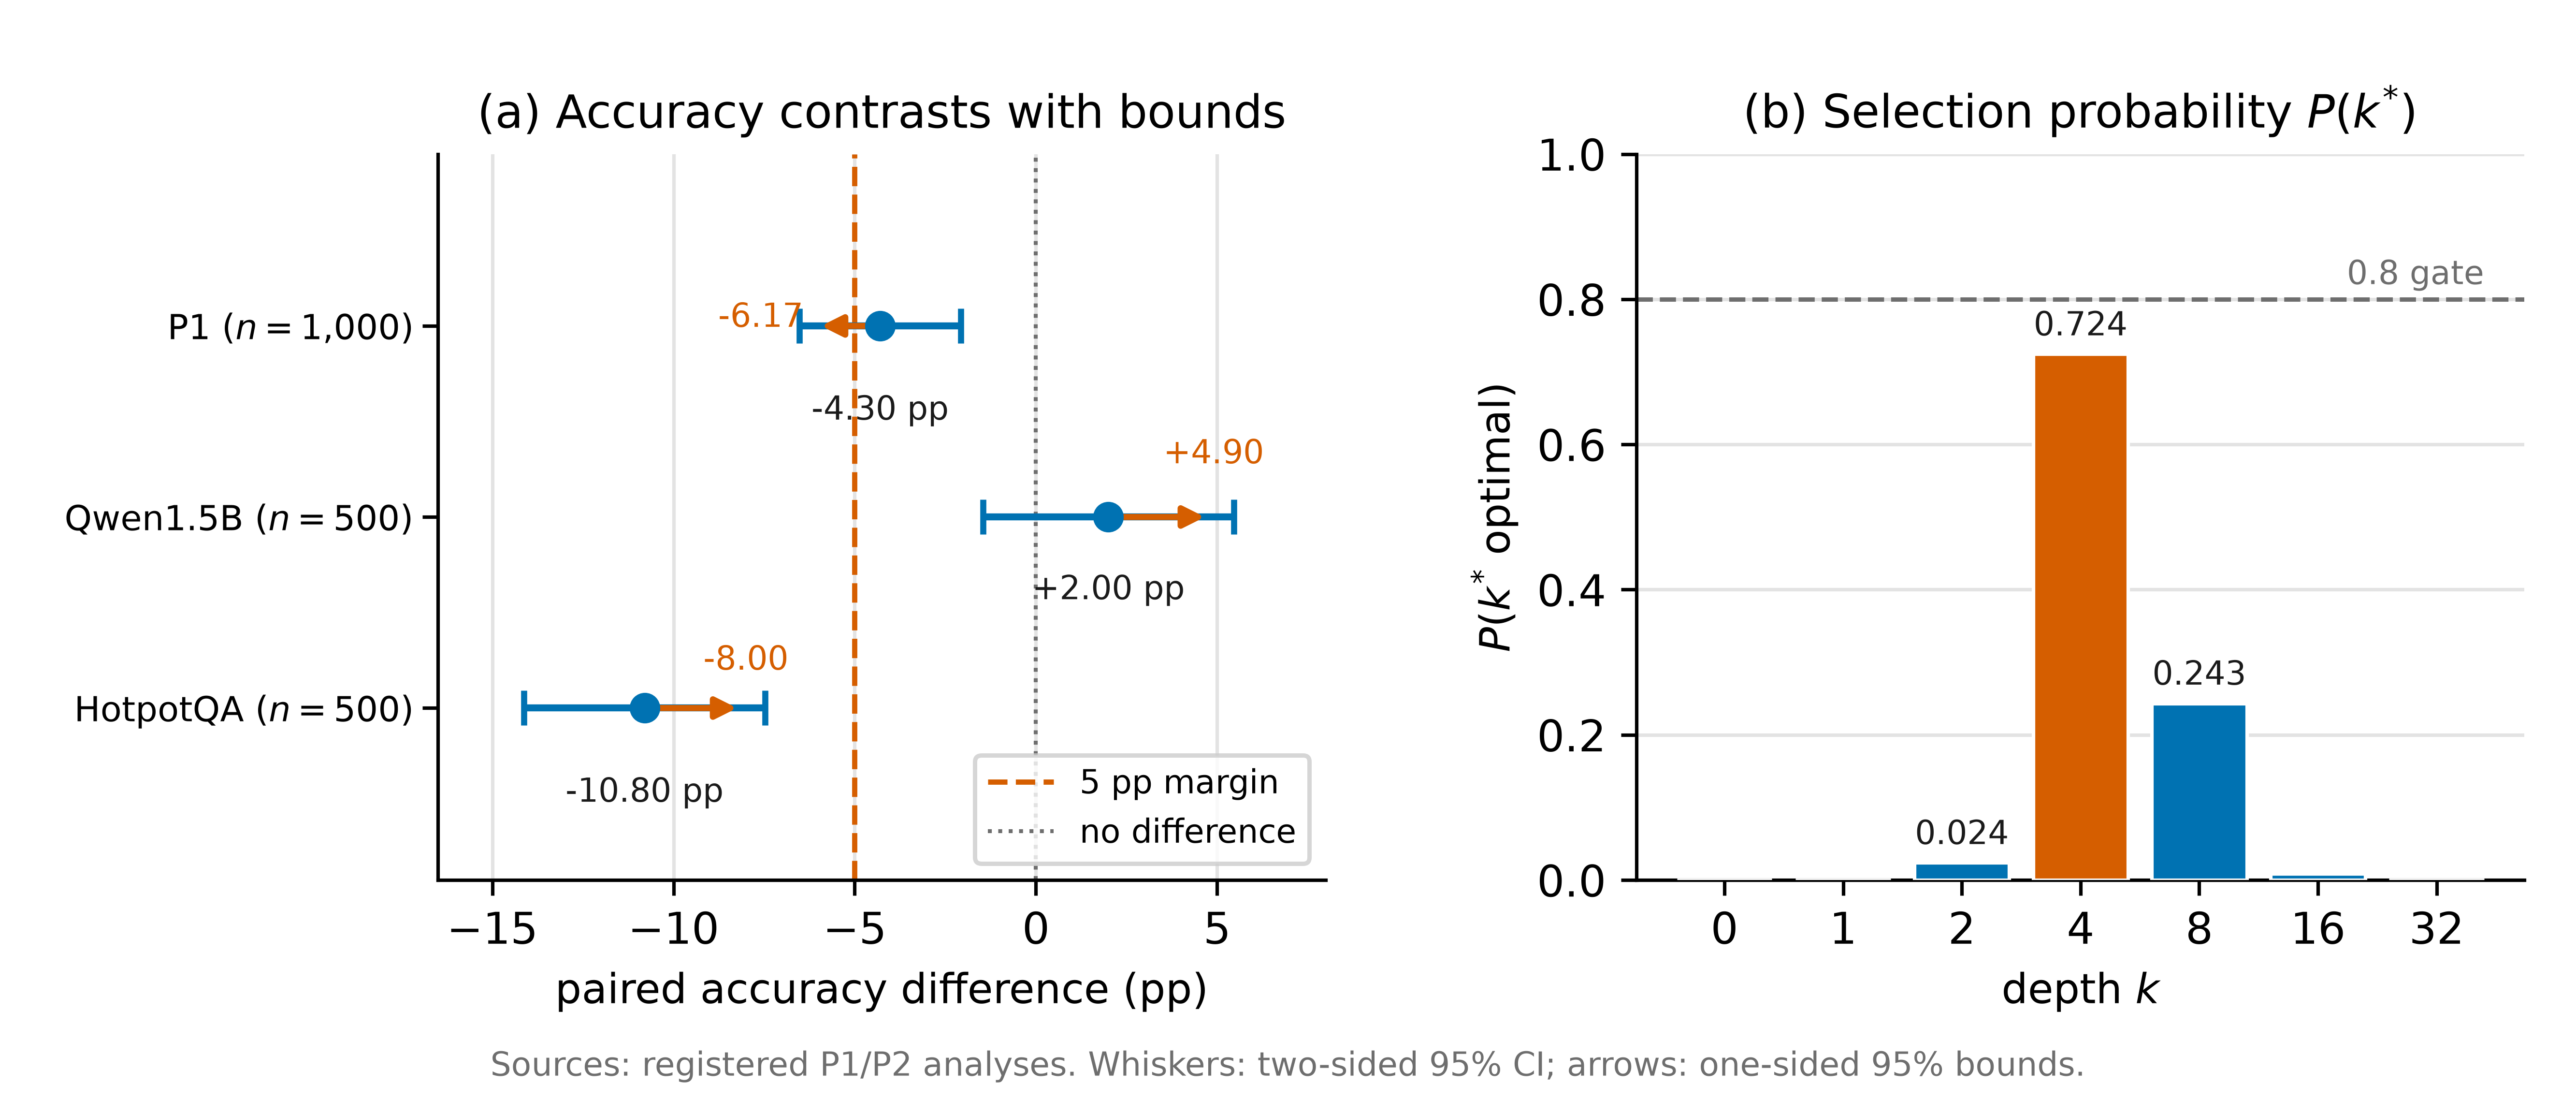
\includegraphics[width=0.98\linewidth]{figures/p1_contrasts.png}}%
    {\missingfigure{figures/p1_contrasts.png}{Accuracy contrasts and selection figure.}}
  \caption{Accuracy contrasts with decision bounds and bootstrap selection. Whiskers are two-sided 95\% intervals; arrows are one-sided 95\% bounds; the dashed line is the 5 pp margin.}
  \label{fig:contrasts}
\end{figure}

\subsection{Theory, Mechanism, and Simulations}\label{sec:p4}

P4 reuses the registered raw CSVs and asks whether the theory travels across
arms; it is descriptive and re-adjudicates no gate. The coverage model
$A(k)=1-(1-a_0)(1-p)^k$ fits poorly on three of four arms (R$^2$ 0.273 on P1,
0.151 on Qwen2.5-1.5B, 0.879 on HotpotQA, and 0.097 on Llama), so it is rejected
as a general description. The Qwen and Llama accuracy curves are non-monotone,
so the distractor counterexample is present in the data and a greedy search that
stops at the first local minimum is not safe. The identity gap is positive at $k\ge4$ on P1, Qwen, and Llama (P1: $+0.200$ at
$k=4$, $+0.703$ at $k=32$), consistent with over-retrieval, while HotpotQA is
negative at $k=2$ and positive from $k=4$. The identity remains a local
diagnostic; it does not establish a global optimum on any arm. A continuous
interpolation resolves the P1 H3 failure: the unconstrained optimum is
$k^{*}=1.214$ with a numerically zero identity gap, so the positive gap at the
gate-selected $k=4$ is over-retrieval relative to that optimum, not a failure of
the identity. This is exploratory and does not re-adjudicate H3. Margin and scoring sensitivity for P1 are in Table~\ref{tab:p1sens}; P4 finds the same rule-dependence on every arm, so the selected depth depends on the scoring rule on every arm.

\begin{figure}[pos=htbp]
  \centering
  \IfFileExists{figures/p1_frontier.png}%
    {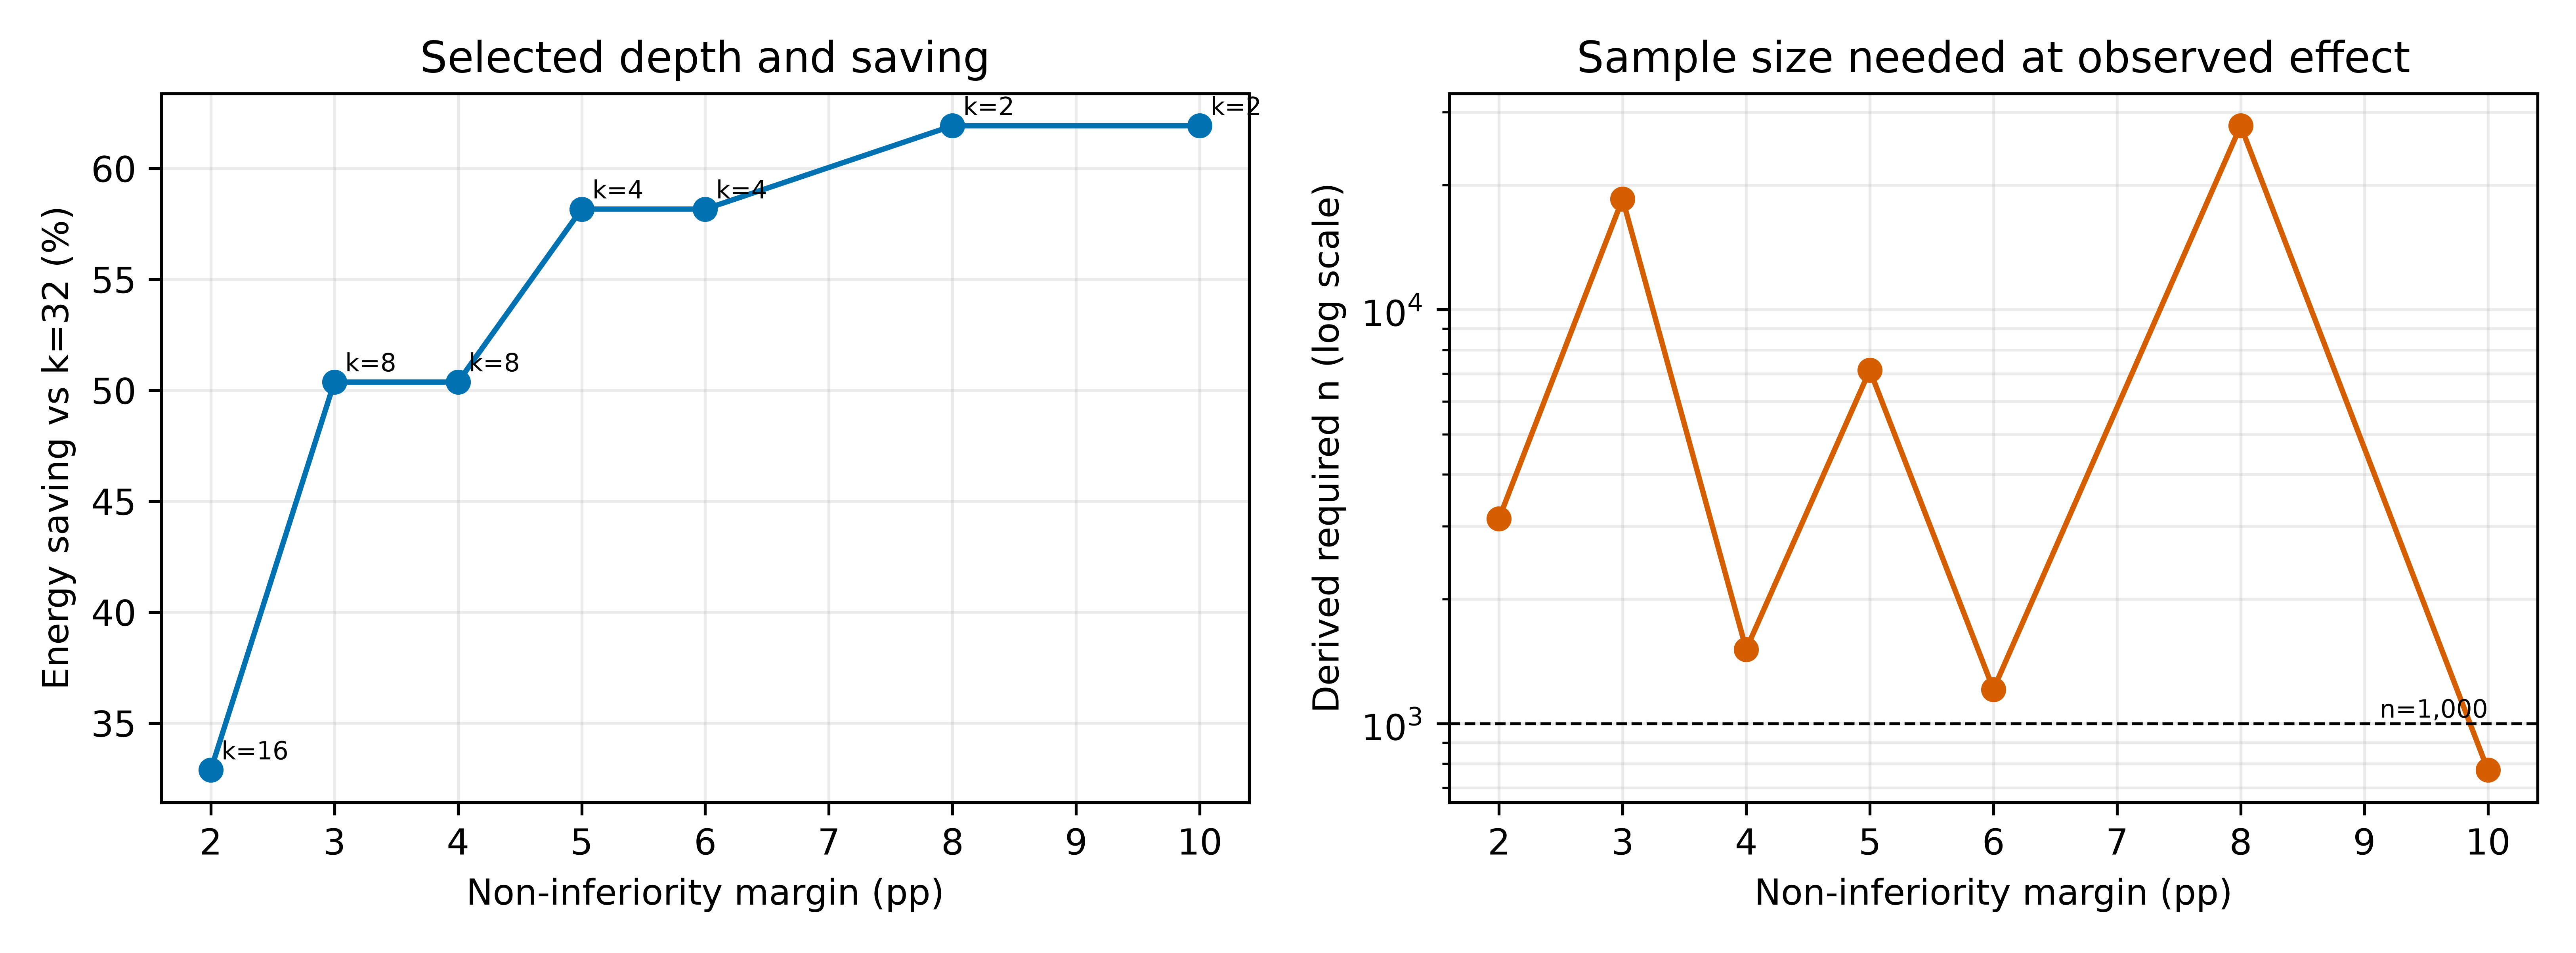
\includegraphics[width=0.98\linewidth]{figures/p1_frontier.png}}%
    {\missingfigure{figures/p1_frontier.png}{Margin-frontier figure generated from the registered analysis.}}
  \caption{Margin-indexed certification frontier: selected depth, energy saving, and derived sample size at each margin.}
  \label{fig:frontier}
\end{figure}

Figure~\ref{fig:frontier} makes the budget explicit. At the observed effect, the 5 pp margin needs about 7{,}100 pairs, the 6 pp margin about 1{,}200, and the 3 pp margin about 18{,}500; only the 10 pp margin clears at $n=1{,}000$. These are derived extrapolations at the observed discordance, not new tests, and the 5 pp row is the only confirmatory one. The practical lesson is that the binding uncertainty is the effect size, not the nominal sample size: a design planned at a near-zero difference cannot resolve a margin that the data show is several percentage points wide.

\label{sec:recallprecision}

Accuracy decomposes as $A(k)=R(k)Q(k)$, where $R(k)$ is the fraction of questions whose answer evidence is in the top-$k$ passages and $Q(k)$ is the conditional probability of a correct answer given that evidence. Table~\ref{tab:rq} reports the decomposition. Recall rises with depth on every arm, while conditional precision falls on SQuAD and Llama; their product produces the plateau. HotpotQA is the opposite regime: both recall and precision rise because multi-hop questions need the second supporting paragraph.

\begin{table}[pos=htbp]
  \centering
  \caption{Recall $\times$ precision decomposition. Two-stage RMSE is for $A=R(q_0-\gamma k)$; one-stage RMSE is for the coverage model.}
  \label{tab:rq}
  \footnotesize
  \begin{tabular}{@{}lrrrrrr@{}}
    \toprule
    \textbf{Arm} & $R(1)$ & $R(\max)$ & $Q(1)$ & $Q(\max)$ & \textbf{2-stage} & \textbf{1-stage} \\
    \midrule
    P1 Qwen4B & 0.590 & 0.892 & 0.663 & 0.553 & \textbf{0.017} & 0.137 \\
    Qwen1.5B & 0.622 & 0.900 & 0.508 & 0.378 & \textbf{0.015} & 0.109 \\
    Llama 3B & 0.622 & 0.900 & 0.669 & 0.473 & \textbf{0.021} & 0.149 \\
    HotpotQA & 0.740 & 1.000 & 0.270 & 0.518 & \textbf{0.024} & 0.062 \\
    \bottomrule
  \end{tabular}
\end{table}

Figure~\ref{fig:rq} shows the decomposition. The SQuAD plateau is a precision decline, not a retrieval ceiling. The Llama peak at $k=4$ is a steeper precision decline. The P3 policy fails because BM25 features predict $R$, not $Q$; the missing signal is reader-side. The two-stage fit is also much tighter than the one-stage coverage model on every arm: RMSE 0.015--0.024 against 0.062--0.149. The model is descriptive and is not used for any decision.

\textbf{Cancellation, not a ceiling.} Table~\ref{tab:cancel} splits the change from $k=4$ to the maximum depth into a recall term and a precision term. The recall term is stable at $+2.4$ to $+6.9$~pp on all four arms; the precision term ranges from $-12.0$ to $+8.4$~pp. The net change is their sum, so the sign of the depth effect is set by precision, not recall. On SQuAD the terms nearly cancel, which is why the 5~pp point estimate sits close to zero and why selection flips between $k=4$ and $k=8$; on HotpotQA both terms are positive and the effect is large. A direct test uses the 590 questions whose gold passage is retrieved first: holding gold at rank~1 and adding 31 distractors lowers exact match from 0.653 to 0.615, a loss of 3.73~pp (95\% CI 0.73 to 6.72). The loss cannot be a retrieval failure, because the answer is already in the prompt; it is reader overload.

\begin{table}[pos=htbp]
  \centering
  \caption{Recall/precision decomposition from $k=4$ to the maximum depth, in percentage points. The two terms sum to the net change in accuracy.}
  \label{tab:cancel}
  \footnotesize
  \begin{tabular}{@{}lrrrrr@{}}
    \toprule
    \textbf{Arm} & $\Delta R$ & $\Delta Q$ & $Q(4)\Delta R$ & $R(\max)\Delta Q$ & \textbf{Net} \\
    \midrule
    P1 Qwen4B (4$\to$32) & $+11.7$ & $-2.8$ & $+6.8$ & $-2.5$ & $+4.3$ \\
    Qwen1.5B (4$\to$32) & $+11.4$ & $-8.0$ & $+5.2$ & $-7.2$ & $-2.0$ \\
    Llama 3B (4$\to$32) & $+11.4$ & $-13.3$ & $+6.9$ & $-12.0$ & $-5.0$ \\
    HotpotQA (4$\to$10) & $+5.6$ & $+8.4$ & $+2.4$ & $+8.4$ & $+10.8$ \\
    \bottomrule
  \end{tabular}
\end{table}

\begin{figure}[pos=htbp]
  \centering
  \IfFileExists{figures/rq_curves.png}%
    {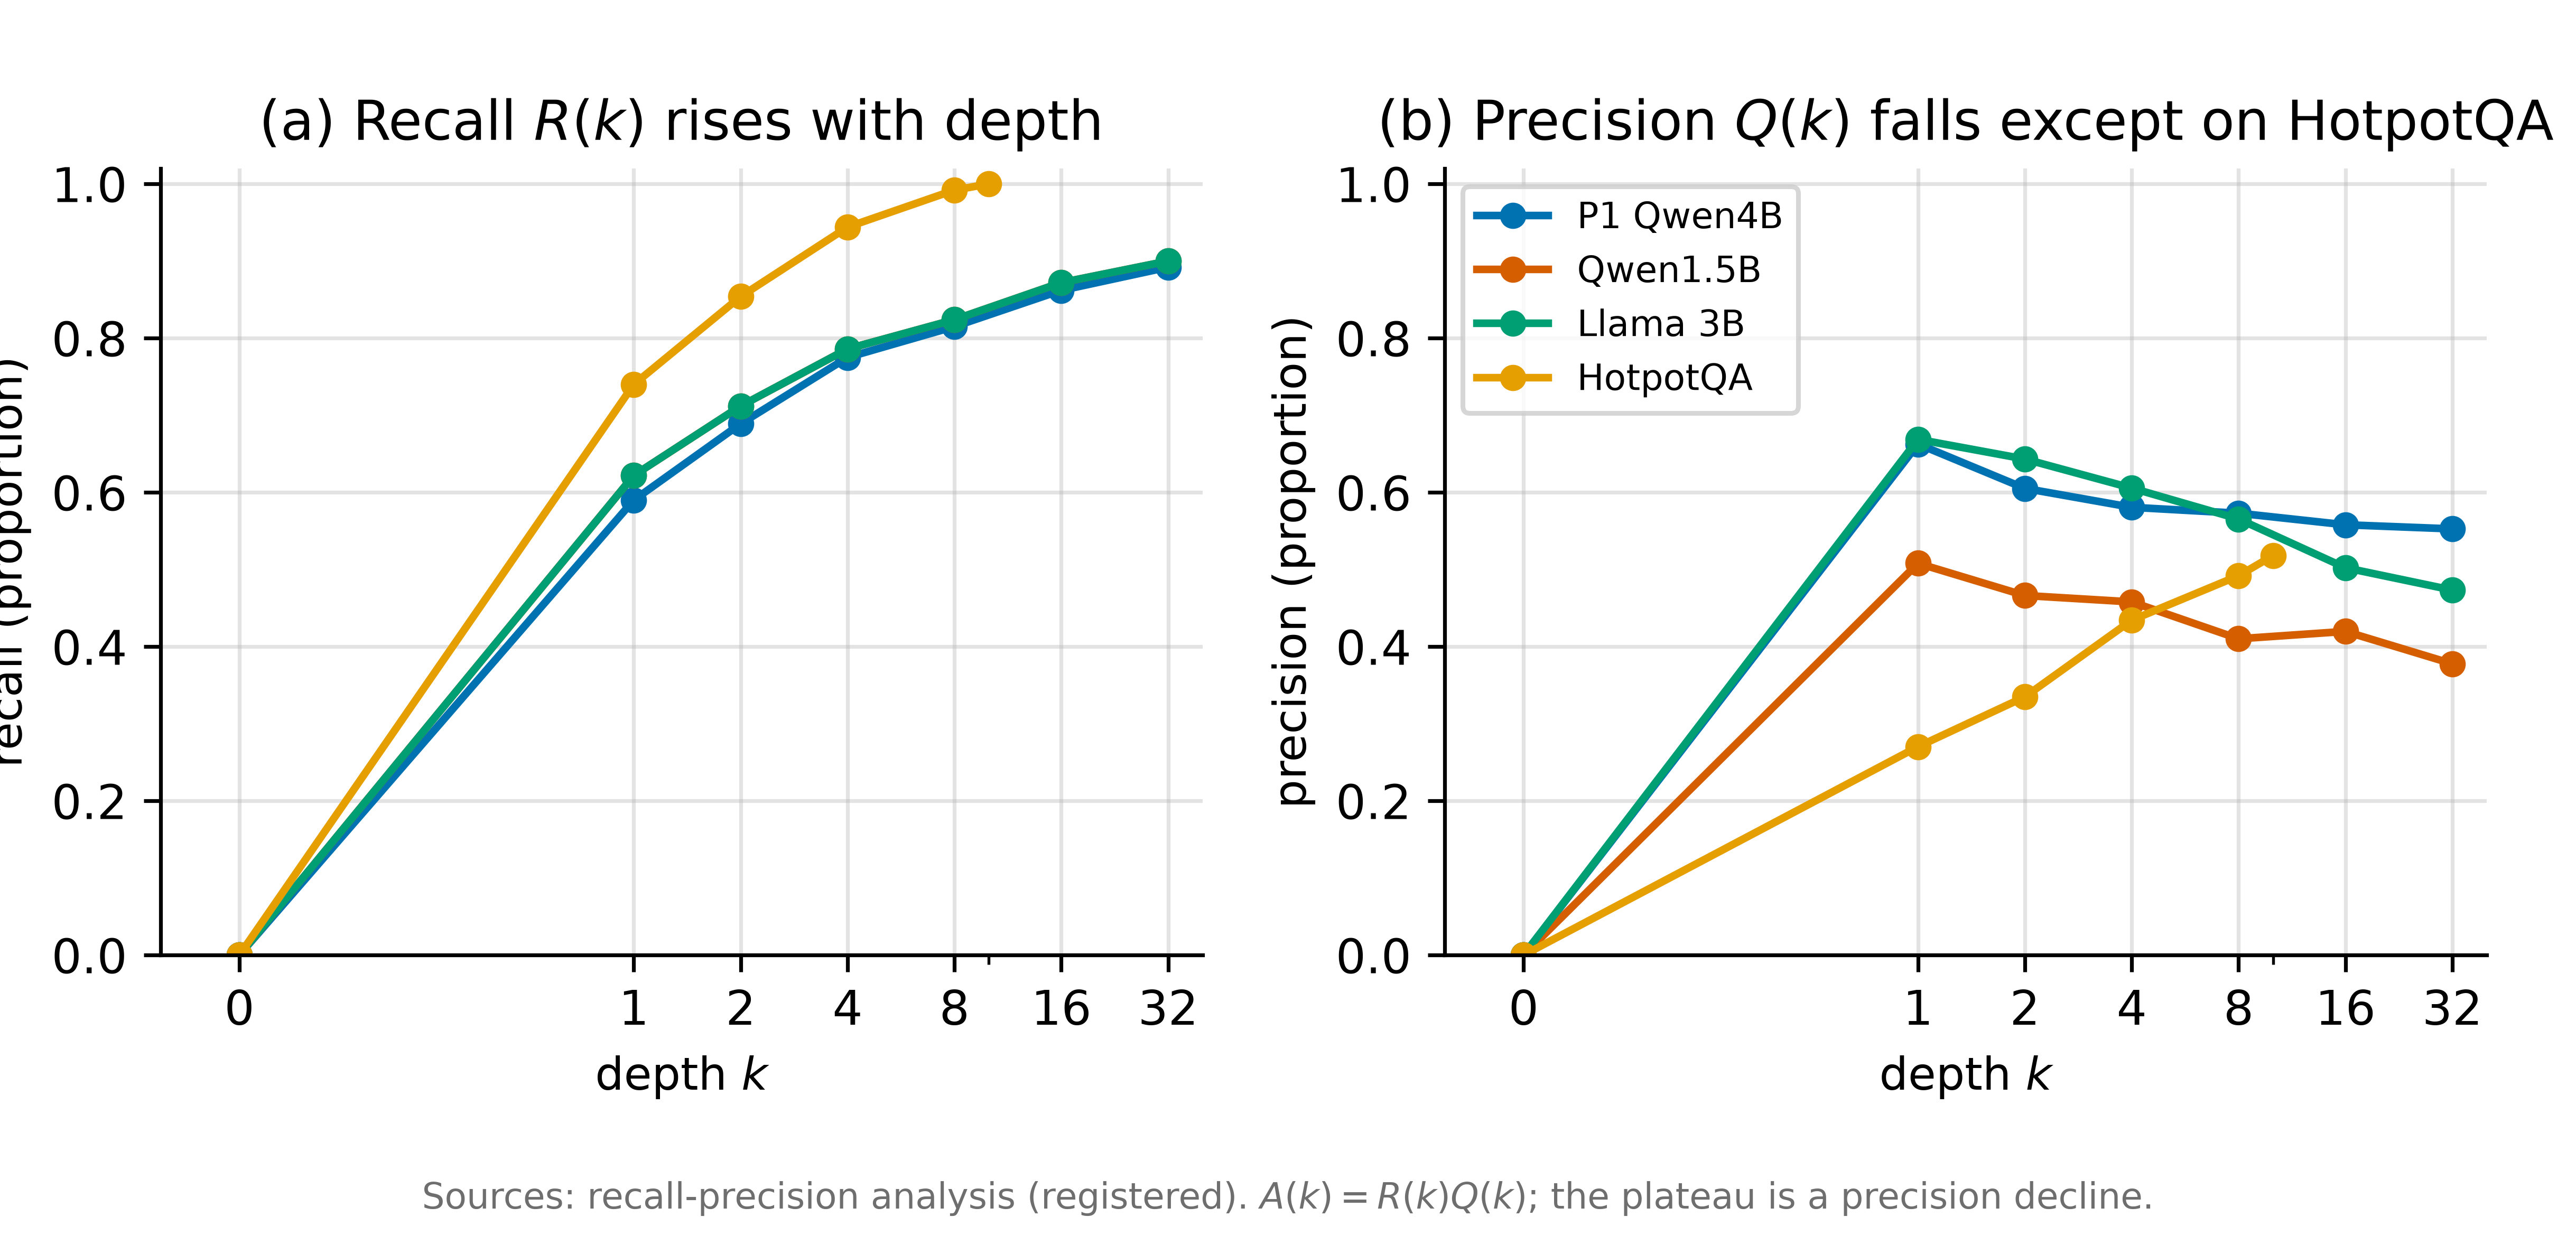
\includegraphics[width=0.98\linewidth]{figures/rq_curves.png}}%
    {\missingfigure{figures/rq_curves.png}{Recall and precision curves.}}
  \caption{Recall rises with depth on all arms while conditional precision falls except on HotpotQA; their product is the accuracy plateau.}
  \label{fig:rq}
\end{figure}

\label{sec:simulations}

\textbf{Mechanism is reader-side.} Holding the gold first and appending 0--31 distractors raises accuracy monotonically on fresh rank-1 questions (0.382 to 0.528, trend $+3.06$~pp per doubling $[1.43, 4.69]$), while the same manipulation lowers it by 3.73~pp on the 590 questions the reader already answers at 0.65 with gold alone: overload is not uniform. A frozen MiniLM ranker leaves the shape unchanged (DiD $-2.20$~pp $[-5.40, +1.00]$, null): the knee does not travel with the retriever. Padding $k=4$ prompts to $k=32$ length recovers 87\% of $k=32$ energy (75.93 vs 87.22~J/q), and P1 timing gives $J=13.88+0.02549T_{\mathrm{pre}}+1.135T_{\mathrm{dec}}$ ($R^{2}=0.9575$ vs $0.8965$): energy follows prompt tokens at about 25~mJ each.

The estimators were exercised on synthetic data, which is a Monte Carlo check rather than new evidence about RAG. The ratio of sums has relative bias 4.9\% at $A=0.1$ and $n=200$, falling to 0.4\% at $n=2{,}000$, whereas the mean of per-question ratios is biased by $-98.7$\% at $A=0.1$; this is the formal reason the paper uses a ratio of sums. At the 5~pp margin the one-sided test rejects at 4.8--6.5\% under the null with power 33.9\% at $n=200$ and 98.9\% at $n=2{,}000$, and with a 2--25\% true gap the selection rate for the true depth is 32--63\% against a 0.8 gate, so $N^{*}$ is biased low by 20\% at $n=200$ and 2\% at $n=1{,}000$. These are descriptive properties of the estimator, not deployment guarantees.

P3 tested whether a query-conditional policy can capture the oracle gap on the hashed 608/206/186 split. The BM25-feature logistic policy reaches 0.4194 accuracy at 59.99~J/correct, while the static $k=1$ baseline reaches 0.4194 at 59.57~J/correct, a saving of $-0.71$\%. Against the matched no-abstention gap of 7.21\% that is a capture of $-9.8$\% (95\% CI $-22.8$ to $-1.8$). The abstention-inclusive gap of 28.64\% is a coverage gain, not depth routing: with fixed per-depth costs the same oracle has a zero gap against $k=1$, because every question already starts at the cheapest depth. Most of the apparent adaptive advantage is therefore abstention, and the remainder is not reachable from BM25 features. G4 is not supported, and no adaptive claim is made.

\subsection{Discussion, Threats, and Limitations}\label{sec:discussion}\label{sec:discussion-body}\label{sec:threats}\label{sec:limitations}\label{sec:status}

P1 is complete and its result is mixed. The measurement chain passed: 7{,}000 of 7{,}000 rows, all seven block factors in range, an idle CV of 1.23\%, and a repeat CV below the 20\% threshold. The descriptive energy model is supported: the per-query curve is affine with $b>0$, $R^{2}=0.9714$, and a lack-of-fit $p$ of 0.2813, and the context share rises from 0.209 to 0.807. The policy claim fails: the accuracy lower bound is outside the 5 pp margin, the selection probability is 0.7244, and the identity gap at $k=4$ excludes zero. The 2 pp margin remains dead, and the 5 pp margin is now also unsupported. P2 is complete. Its 1.5B-reader arm does not support H7 ($+2.00$ pp, upper $+4.90$ pp), while the HotpotQA arm does ($-10.80$ pp, upper $-8.00$ pp) and satisfies G5. Energy on both P2 arms is uncalibrated because at least one block factor failed, so the P2 energy contrasts are not certified. P3 is complete and negative on G4; its policy does not capture the oracle gap (Section~\ref{sec:p4}). P4 is descriptive: the coverage model is rejected on three of four arms, Qwen and Llama are non-monotone, and positive identity gaps at $k\ge4$ flag over-retrieval without certifying a global optimum. Table~\ref{tab:claims} collects the claim-to-evidence map. Each row states the estimate, its uncertainty, the status, and what would falsify it. The table is the compact form of the paper's argument: the measurement and descriptive claims survive, the 5 pp policy claim does not, the direction holds on HotpotQA and is inconclusive on the 1.5B reader, the adaptive gate fails, and the theory is local.

\begin{table}[pos=htbp]
  \centering
  \caption{Claim-to-evidence map. Status is fixed by the preregistration and is not re-thresholded.}
  \label{tab:claims}
  \scriptsize
  \setlength{\tabcolsep}{3pt}
  \begin{tabular}{@{}>{\raggedright\arraybackslash}p{2.8cm}>{\raggedright\arraybackslash}p{3.9cm}>{\raggedright\arraybackslash}p{3.4cm}>{\raggedright\arraybackslash}p{2.3cm}>{\raggedright\arraybackslash}p{2.8cm}@{}}
    \toprule
    \textbf{Claim} & \textbf{Estimate} & \textbf{Uncertainty} & \textbf{Status} & \textbf{Falsifier} \\
    \midrule
    H1: energy is affine in depth & $J=26.90+2.149k$ ($k\ge1$); token model $R^{2}=0.902$ & 95\% CIs; lack-of-fit $p=0.2813$ & supported & curvature or negative $b$ \\
    H2: 5 pp static policy & $A(4)-A(32)=-4.30$ pp & one-sided lower $-6.17$ pp; $p=0.2691$ & not supported & lower bound above $-5$ pp \\
    Accuracy cost is nonzero & $-4.30$ pp & two-sided 95\% CI $[-6.53,-2.07]$; McNemar $p=0.0002$ & supported & interval includes zero \\
    H3: identity at $k=4$ & $\Delta(4)=+0.2004$ & 95\% CI $[0.1677,0.2320]$ & not supported & interval includes zero \\
    Continuous optimum & $k^{*}=1.214$, $\Delta\approx0$ & interpolation diagnostic & exploratory & curve not concave near optimum \\
    H4: context share rises & $S(4)=0.355$; 0.209 to 0.807 & bootstrap interval & supported & flat or falling share \\
    H7 on Qwen1.5B & $+2.00$ pp & upper $+4.90$ pp & not supported & negative interval \\
    H7 on HotpotQA & $-10.80$ pp & upper $-8.00$ pp & supported & interval crosses zero \\
    G5 external validity & HotpotQA direction & one-sided upper $-8.00$ pp & pass & both arms fail \\
    G4 adaptive policy & 28.64\% matched oracle; policy $-9.8$\% & 95\% CI $-22.8$ to $-1.8$; AUC 0.733 & fail & policy capture $\ge50$\% \\
    Coverage model & $R^{2}$ 0.097--0.879 & model rejected on 3/4 arms & rejected & good fit on all arms \\
    Recall $\times$ precision & two-stage RMSE 0.015--0.024 & versus 0.062--0.149 one-stage & descriptive & two-stage worse than one-stage \\
    P2 energy & sweep/block range & uncalibrated; window bias & descriptive & calibrated replay agrees \\
    \bottomrule
  \end{tabular}
\end{table}

\textbf{Observation.} P1 gives a calibrated curve, with absolute $J$ provisional after the window-bias audit: energy per correct answer rises from 73.71 J at $k=1$ to 192.59 J at $k=32$ (2.61$\times$), the per-query curve is affine with $R^{2}=0.9714$, and the context-side share rises from 0.209 to 0.807. The primary accuracy contrast is $-4.30$ pp with a one-sided lower bound of $-6.17$ pp, and the saving is 58.17\% on the window estimator (95\% interval [56.02, 60.14]\%) and 65.25\% on the block estimator ([61.27, 69.11]\%). The selection probability is 0.7244 at $k=4$ and 0.2433 at $k=8$, the identity gap at $k=4$ is $+0.2004$ with an interval that excludes zero, and $N^{*}$ is a descriptive break-even of 6{,}189 queries.

\textbf{Interpretation.} The point estimate is inside the 5 pp margin by 0.70 pp, but the one-sided lower bound is outside it by 1.17 pp, so non-inferiority is not established. The result is a precision failure at $n=1{,}000$, not proof that the true loss exceeds 5 pp. It is, however, evidence of a real cost: the two-sided interval excludes zero and the McNemar test rejects equality ($p=0.0002$), so the data support “depth reduction is not free” even though they do not settle “the loss is at most 5 pp.” The observed discordance is 13.1\%, above the 8\% used in the planning calculation, so the realized interval is wider than the design assumed; the power calculation was conditional on a rate that the run did not reproduce. The energy side is not the problem. A 58.17\% saving is large and its interval is far above the 20\% floor, but the policy decision requires both conditions, and the accuracy gate is the binding one. The pilot's 69.3\% signal did not replicate as a supported claim: the saving is smaller at 58.17\% and the accuracy bound does not clear the margin. The descriptive energy result replicated; the policy result did not.

\textbf{Selection stability and identity.} The selected depth is unstable between $k=4$ and $k=8$. The source is visible in the point estimate: $k=4$ clears the accuracy gate by only 0.70 pp, so a small resampling movement in $A(4)$ makes $k=8$ the smallest feasible depth, and $k=8$ has a higher $E$. K3 fails on the 0.8 selection threshold and K5 fails because the 95\% span covers both depths. Figure~\ref{fig:contrasts}(b) shows the split: 0.7244 at $k=4$ against 0.2433 at $k=8$. The identity gap is positive at $k=4$, which says that the energy elasticity exceeds the accuracy elasticity and that the gate-selected depth lies above the unconstrained energy optimum. This is consistent with a gate that binds at the smallest feasible depth rather than a contradiction of the policy result. Both diagnostics point the same way: the static selection is driven by the margin, not by an interior energy minimum, so it is fragile to the accuracy estimate. No universal $k^{*}$ follows, and the instability is a reason not to report one. \textbf{Measurement.} P0 failed block calibration; P1 passed all seven factors, so the absolute energy scale is reportable as provisional for P1 under the window-bias audit (D-028). The pass is not comfortable. The $k=0$ factor, 0.8089, is only 1.1\% above the fixed floor, and $k=0$ is the depth with the least stable accuracy (one correct answer in 1{,}000), so the intercept $a=24.0759$ is the least well identified parameter of the fit. The 25.9\% discrepancy that failed P0 is exactly the kind of error the gate is designed to catch; the P1 pass shows that the revised protocol can work, not that the calibration is comfortable. The wall meter remains waived (D-016), so the GPU integration is not cross-checked against system energy.

\textbf{Implication for practice.} The static 5 pp rule is not supported on this evidence. A deployment that needs a 5 pp accuracy guarantee should not adopt $k=4$ on the basis of this run, even though the point estimate saves 58.17\% of energy per correct answer. The margin-indexed decision procedure remains the right object: state the margin, measure the curve on the target corpus and reader, and test the candidate. The sensitivity analysis shows what that procedure returns at other margins: $k=16$ at 2 pp with 32.9\% savings, $k=8$ at 3--4 pp with 50.4\%, $k=4$ at 5--6 pp with 58.2\%, and $k=2$ at 8--10 pp with 61.9\%. These are point estimates from one sample, not guarantees, and no rule selects $k=32$.

\textbf{Relation to the adaptive direction.} The static claim fails, so P3 tested whether a query-conditional policy can recover the oracle gap. The answer on this feature set is no: the BM25-feature policy saves $-0.71\%$ (capture $-9.8\%$), so G4 is not supported, and most of the oracle advantage is an abstention gain rather than depth routing. The negative result is for this policy class, not a proof that no adaptive policy can work.

\textbf{Hardware and measurement.} All energy measurements come from one laptop GPU. The pilot reached 88.4~$^{\circ}$C and a 1003~MHz clock, and P0 reached 90~$^{\circ}$C with a 900~MHz clock floor, so the device is thermally throttled during long runs. NVML updates \texttt{power.draw} at roughly 1~s despite the 100~ms cadence, so per-query energy is a paired observation rather than a precision measurement. Block calibration failed in P0 and passed in P1, but the $k=0$ factor is 0.8089, only 1.1\% above the floor, and the repeat CV maximum is 18.44\%, close to the 20\% threshold. No wall meter is available (D-016, D-031), and the CPU retrieval term is a 20~W time-to-joules proxy. \textbf{What the metrology audit establishes.} The replay and session audits in Section~\ref{sec:pilot} show that a continuous sequence absorbs a thermal transient that a cooldown-separated block design does not, so a single replay landing within 2\% of the block sum was a coincidence rather than a validation, and that the absolute joule level varies 3.3--5.9\% between measurement occasions on identical questions at identical accuracy. No absolute figure in this paper should therefore be read as a deployment guarantee; the saving is the reproducible quantity. The shared H200 slice cannot supply an energy measurement at all because per-instance power telemetry is unavailable, so it is used for accuracy only. Every joule reported here is GPU energy from NVML; no system or wall energy is claimed. \textbf{Design and scope.} The study uses one corpus (SQuAD v1.1), one retriever (BM25), one reader family, and a 4-bit quantized model at a 4096-token context with $k\le32$. SQuAD is a closed-corpus extractive task, so the results do not automatically transfer to open-domain generation, dense retrieval, long-context readers, or API models. The boundary probe at $k\in\{32,48,64\}$ and the context-budget probe were run in P2 and are diagnostic; neither is a new $k^{*}$. The Llama 3.2 3B reader is exploratory and does not satisfy the replication gate. The P2 Qwen arm failed block calibration at $k=0,1,2$ and its repeat CV reached 80.15\%, so its energy contrast is uncalibrated; the HotpotQA arm missed only $k=0$ but is also uncalibrated because calibration is all-or-nothing. P4 shows the accuracy curve is not generally monotone or well described by the coverage model, so the identity and any greedy search are local diagnostics rather than global guarantees. The accuracy metric is normalized exact match, which is conservative and does not credit paraphrases; the scoring sensitivity shows that the selected depth changes under lenient span and token F1, so the result is rule-dependent. The pilot used strict exact match, so pilot and P1 accuracy values are not like-for-like. A single run seed controls the within-question depth order, and seed-to-seed variability is not estimated.

\textbf{Statistical power.} The planning calculation assumed an 8\% discordant rate and an interval half-width of about 1.8 pp at $n=1{,}000$. The run produced 13.1\% discordance, so the realized interval is wider and the 5 pp margin was not resolved. The design can estimate a difference of this size but did not establish the margin; a larger sample, or a lower-discordance reader, would be needed to do so, and the required size depends on the discordance rate that was observed. The 2 pp margin is dead at this sample size and remains estimation-only. The selection probability is a bootstrap quantity and inherits the uncertainty of the curve. Secondary estimands are not corrected for multiplicity because only one confirmatory test is declared, and they are labelled accordingly. \textbf{Identity and selection.} H3 is not supported: the identity gap at $k=4$ is $+0.2004$ with an interval that excludes zero. The identity is a diagnostic, not a policy gate, and its failure says that the selected depth is not an unconstrained energy optimum. K3 and K5 fail because the selection is unstable between $k=4$ and $k=8$. Neither failure invalidates the descriptive curve, but both limit any claim that a particular static depth is the best one.

\textbf{Status.} The confirmatory result is negative on the primary policy claim and positive on the measurement and descriptive claims. P2 is complete: the direction holds on HotpotQA and is inconclusive on the 1.5B reader, and the P2 energy contrasts are uncalibrated. P3 is complete and negative on G4: the learned policy does not capture the oracle gap, so no adaptive claim is made. P4 is descriptive and rejects the coverage model as a general description. \textbf{Data and reproducibility.} Raw SQuAD text is not redistributed, and the raw run directories are local-only under D-020. The repository publishes the dataset IDs, checksums, configs, prompts, split IDs, predictions, and aggregate statistics, and the public code/analysis archive is at DOI \texttt{10.5281/zenodo.24352803}. Sanitized per-query tables in \texttt{artifacts/release/} omit question text, gold answers, predictions, and nonces but retain question IDs, depth, correctness flags, and measured joules, so a reader can rebuild the energy and accuracy tables without redistributing the benchmarks.

\section{Conclusion}\label{sec:conclusion}

The paper asked whether an interior retrieval depth can replace the retriever's ceiling at an acceptable accuracy cost. It treated depth as a decision, estimated energy per correct answer as a ratio of sums, and tested a preregistered 5 pp margin at $k=4$ against $k=32$ on 1{,}000 SQuAD questions with a calibrated single-GPU protocol. The 5 pp claim is not supported: $k=4$ lost 4.30 pp (lower bound $-6.17$ pp), saving 58.17\% (window) and 65.25\% (block) of GPU energy per correct answer. The energy curve, affine fit, and rising context share are supported, but selection is unstable and the identity gap is positive at $k=4$. Three mechanism probes agree the effect is reader-side: gold-first distractors raise accuracy ($+14.6$~pp), the knee survives a retriever swap, and length-matched padding recovers 87\% of $k=32$ energy, pricing prompt tokens at about 25~mJ each. Depth reduction has a measurable accuracy cost here; no universal $k^{*}$ or adaptive-policy gain follows.

\printcredits

\section*{Declarations}
\begin{itemize}
  \setlength{\itemsep}{0pt}
  \setlength{\parsep}{0pt}
  \item \textbf{Funding:} This research received no external funding.

  \item \textbf{Conflicts of Interest:} The authors declare that they have no known competing financial interests or personal relationships that could have appeared to influence the work reported in this paper.

  \item \textbf{Data availability:} Raw SQuAD text is not redistributed; SQuAD remains under CC BY-SA 4.0. The repository publishes the dataset identifiers, versions, SHA-256 checksums, split identifiers, configs, prompts, predictions, and aggregate statistics. Raw run directories are local-only under decision D-020, with an external backup recorded in D-027. The P0 and P1 run registry rows and the tracked energy ledger are public. Sanitized per-query tables in \texttt{artifacts/release/} retain question IDs, depth, correctness, and joules but omit text, gold answers, predictions, and nonces; they rebuild the energy and accuracy tables without redistributing the benchmarks. The public code/analysis archive is at \url{https://doi.org/10.5281/zenodo.24352803}.

  \item \textbf{Code availability:} The measurement harness, analysis code, and configuration schema are available at \url{https://github.com/Atik203/energy-optimal-rag} and archived at \url{https://doi.org/10.5281/zenodo.24352803} under the MIT license. Documentation and derived artifacts are released under CC BY 4.0.

  \item \textbf{Ethical approval:} No human-subject data were collected. The study uses public benchmark questions and locally generated model answers.

  \item \textbf{Models and inference:} The reader is a local 4-bit quantized language model. No API reader and no paid inference service is used in any reported measurement.
\end{itemize}

\section*{Acknowledgements}
The authors thank the curators of SQuAD for releasing the dataset under CC BY-SA 4.0, and the maintainers of Ollama, BM25 implementations, and NVML for the tooling that made the measurement possible. All computations were run on a single local laptop GPU; no cloud compute was used.

\hbadness=10000
\sloppy
\setlength{\bibsep}{0pt}
\renewcommand{\bibfont}{\fontsize{8.5pt}{9pt}\selectfont}
\bibliographystyle{elsarticle-num}
\bibliography{refs}

\vspace{4pt}
\end{document}
